%-------------------------------------------------------%
%       Snakemake-Intro for HPC Users                   %
%-------------------------------------------------------%


% this code will compile the document as handout with
% $ pdflatex -synctex=1 -interaction=nonstopmode "\def\ishandout{1} %-------------------------------------------------------%
%       Snakemake-Intro for HPC Users                   %
%-------------------------------------------------------%


% this code will compile the document as handout with
% $ pdflatex -synctex=1 -interaction=nonstopmode "\def\ishandout{1} %-------------------------------------------------------%
%       Snakemake-Intro for HPC Users                   %
%-------------------------------------------------------%


% this code will compile the document as handout with
% $ pdflatex -synctex=1 -interaction=nonstopmode "\def\ishandout{1} %-------------------------------------------------------%
%       Snakemake-Intro for HPC Users                   %
%-------------------------------------------------------%


% this code will compile the document as handout with
% $ pdflatex -synctex=1 -interaction=nonstopmode "\def\ishandout{1} \input{Snakemake_HPC_Users.tex}"
\ifdefined\ishandout
\PassOptionsToClass{handout}{beamer}
\fi

\documentclass[english,xcolor=pdftex,dvipsnames]{beamer} 

% to typeset only a few slide sets, set them here during development
%\includeonly{Why_Workflows}

\input{common/preamble}

\title[<++course.shorttitle++>]{<+++ if course.title is defined +++><++course.tittle++><+++else+++>An Introduction to HPC-conformant Scientific Workflows with \Snakemake<+++endif+++>} 

\subtitle{<+++ if course.subtitle is defined +++><++course.subtitle++><+++else+++>Deployment<+++endif+++> - <++course.edition++>} 

%%%%%%%%%%%%%%%%%%%%%%%%%%%%%%%%%%%%%%%%%%%%%%%%%%%%%%%%%%%%%%%%%%%%%%%%%%%%%%%%
%%%%%%%%%%%%%%%%%%%%%%%%%%%%%%%%%%%%%%%%%%%%%%%%%%%%%%%%%%%%%%%%%%%%%%%%%%%%%%%%
\begin{document}
%%%%%%%%%%%%%%%%%%%%%%%%%%%%%%%%%%%%%%%%%%%%%%%%%%%%%%%%%%%%%%%%%%%%%%%%%%%%%%%%
%%%%%%%%%%%%%%%%%%%%%%%%%%%%%%%%%%%%%%%%%%%%%%%%%%%%%%%%%%%%%%%%%%%%%%%%%%%%%%%%

% attempts a better type setting for hboxes (might result in less overful warnings)
\sloppy

%%%%%%%%%%%%%%%%%%%%%%%%%%%%%%%%%%%%%%%%%%%%%%%%%%%%%%%%%%%%%%%%%%%%%%%%%%%%%%%% 
\begin{frame}[plain] % plain erzeugt Titelseite ohne Kopf- und Fußzeile
  \titlepage
\end{frame}

%%%%%%%%%%%%%%%%%%%%%%%%%%%%%%%%%%%%%%%%%%%%%%%%%%%%%%%%%%%%%%%%%%%%%%%%%%%%%%%%
\include{common/contributions}

%%%%%%%%%%%%%%%%%%%%%%%%%%%%%%%%%%%%%%%%%%%%%%%%%%%%%%%%%%%%%%%%%%%%%%%%%%%%%%%%
\include{common/Why_Workflows}

%%%%%%%%%%%%%%%%%%%%%%%%%%%%%%%%%%%%%%%%%%%%%%%%%%%%%%%%%%%%%%%%%%%%%%%%%%%%%%%%
\include{common/About_Snakemake}

%%%%%%%%%%%%%%%%%%%%%%%%%%%%%%%%%%%%%%%%%%%%%%%%%%%%%%%%%%%%%%%%%%%%%%%%%%%%%%%%
\include{common/Sample_Data}

%%%%%%%%%%%%%%%%%%%%%%%%%%%%%%%%%%%%%%%%%%%%%%%%%%%%%%%%%%%%%%%%%%%%%%%%%%%%%%%%
\include{common/software_environment}

%%%%%%%%%%%%%%%%%%%%%%%%%%%%%%%%%%%%%%%%%%%%%%%%%%%%%%%%%%%%%%%%%%%%%%%%%%%%%%%%
\include{users/Selecting_Workflows}

%%%%%%%%%%%%%%%%%%%%%%%%%%%%%%%%%%%%%%%%%%%%%%%%%%%%%%%%%%%%%%%%%%%%%%%%%%%%%%%%
% \include{common/Using_Workflow_Configs}

%%%%%%%%%%%%%%%%%%%%%%%%%%%%%%%%%%%%%%%%%%%%%%%%%%%%%%%%%%%%%%%%%%%%%%%%%%%%%%%%
\include{common/Plotting_DAGs}

%%%%%%%%%%%%%%%%%%%%%%%%%%%%%%%%%%%%%%%%%%%%%%%%%%%%%%%%%%%%%%%%%%%%%%%%%%%%%%%%
\include{common/HPC_101}

%%%%%%%%%%%%%%%%%%%%%%%%%%%%%%%%%%%%%%%%%%%%%%%%%%%%%%%%%%%%%%%%%%%%%%%%%%%%%%%%
\include{common/Workflow_Parameterization_for_HPC}
      
%%%%%%%%%%%%%%%%%%%%%%%%%%%%%%%%%%%%%%%%%%%%%%%%%%%%%%%%%%%%%%%%%%%%%%%%%%%%%%%%
\include{common/Reports}    

%%%%%%%%%%%%%%%%%%%%%%%%%%%%%%%%%%%%%%%%%%%%%%%%%%%%%%%%%%%%%%%%%%%%%%%%%%%%%%%%
\include{common/using_wrappers}

%%%%%%%%%%%%%%%%%%%%%%%%%%%%%%%%%%%%%%%%%%%%%%%%%%%%%%%%%%%%%%%%%%%%%%%%%%%%%%%%
\include{common/Fine_Tuning}

%%%%%%%%%%%%%%%%%%%%%%%%%%%%%%%%%%%%%%%%%%%%%%%%%%%%%%%%%%%%%%%%%%%%%%%%%%%%%%%%
% \include{common/Contributing} 
\end{document}

"
\ifdefined\ishandout
\PassOptionsToClass{handout}{beamer}
\fi

\documentclass[english,xcolor=pdftex,dvipsnames]{beamer} 

% to typeset only a few slide sets, set them here during development
%\includeonly{Why_Workflows}

\usepackage{etoolbox}
%\setbeamertemplate{mini frames}[box]
\usepackage{babel}
\usepackage[utf8]{inputenc}
\usepackage[T1]{fontenc}
\usepackage{amsfonts,amsmath,amssymb}
\usepackage{textgreek}
\usepackage{wrapfig}

\usepackage[load-configurations=binary,binary-units=true]{siunitx}
\usepackage[normalem]{ulem} % for strikethrough with \sout

\usepackage{color,colortbl}
\usepackage{upquote}

\usepackage{pifont}

\definecolor{pblue}{RGB}{45,106,148}
\definecolor{pdarkblue}{RGB}{35,71,100}
\definecolor{plightblue}{RGB}{90,159,212}
\definecolor{pyellow}{RGB}{255,212,59}
\definecolor{pdarkyellow}{RGB}{255,188,41}
\definecolor{orange}{RGB}{255,165,0}
\definecolor{plightyellow}{RGB}{255,232,115}
\definecolor{pdarkgrey}{RGB}{100,100,100}
\definecolor{pgrey}{RGB}{153,153,153}
\definecolor{plightgrey}{RGB}{233,233,233}
\definecolor{plightgrey2}{RGB}{247,247,247}
\definecolor{pnavy}{RGB}{0,0,170}
\definecolor{BrickRed}{RGB}{150,22,11}
\definecolor{BlueViolet}{RGB}{138, 43, 226}
\definecolor{PineGreen}{RGB}{0, 51, 0}
\definecolor{light-gray}{gray}{0.95}

\definecolor{UniRot}{RGB}{193,0,42}
\definecolor{UniDunkelGrau}{RGB}{99,99,99}
\definecolor{UniHellGrau}{RGB}{172,172,172}

\definecolor{UrlColor}{rgb}{0,0.08,0.45}
\definecolor{links}{rgb}{0,0,0}

\usetheme{<++layout.theme++>} % Pittsburgh, CambridgeUS
\usecolortheme{<++layout.colortheme++>} %wolverine | crane | beaver | seahorse
\useinnertheme{rounded} 
\useoutertheme{default}
\usefonttheme{default}
%\setbeamercovered{transparent}
\setbeamertemplate{footline}[frame number]

% remove the navigation symbols
\setbeamertemplate{navigation symbols}{}

% side margins
\setbeamersize{text margin left=0.5cm, text margin right=0.5cm}

\setbeamercolor{structure}{<++layout.beamercolor_structure++>}% to modify  immediately all palettes
\setbeamercolor{title}{<++layout.beamercolor_title++>}
\setbeamercolor{title in head/foot}{<++layout.beamercolor_title_head++>}

\setbeamercolor{block title}{<++layout.beamercolor_block_title++>}
\setbeamercolor{block body}{<++layout.beamercolor_block_body++>}

% \setbeamercolor{block title}{fg=white,bg=orange}
\setbeamercolor{block title alerted}{<++layout.beamercolor_block_title++>}
\setbeamercolor{block title example}{<++layout.beamercolor_block_title++>}

% enables two line cols in tabular envs
\newcommand{\specialcell}[2][c]{%
  \begin{tabular}[#1]{@{}c@{}}#2\end{tabular}}
\usepackage{subfig}
\usepackage{tikz}
\usetikzlibrary{arrows,shapes,snakes,backgrounds,positioning,shadows,decorations,trees,decorations.pathreplacing, graphs}
\usepackage{tkz-graph}

%\usepackage{tikzpeople}
\usepackage{smartdiagram}
\usesmartdiagramlibrary{additions}

%\usepackage{mdframed}

\usepackage{adjustbox} % to adjust tikzpictures within slides


\addtobeamertemplate{footline}{}{%
\begin{tikzpicture}[remember picture,overlay]
\node[anchor=south west,yshift=2pt] at (current page.south west) {\includegraphics[height=0.8cm]{../images/logos/zdv_logo.png}};
\end{tikzpicture}}

\usepackage[tikz]{bclogo}
\newenvironment{task}[1][Task]{\bclogo[arrondi=0.1,logo=\bcoutil]{#1}}{\endbclogo}
\newenvironment{docs}[1][Documentation]{\bclogo[arrondi=0.1,logo=\bcplume]{#1}}{\endbclogo}
\newenvironment{hint}[1][Hint]{\bclogo[arrondi=0.1,logo=\bcinfo]{#1}}{\endbclogo}
\newenvironment{warning}[1][Warning]{\bclogo[arrondi=0.1,logo=\bcattention]{#1}}{\endbclogo}
% ``d/Definition'' is already defined ;-)
\newenvironment{explanation}[1][Definition]{\bclogo[arrondi=0.1,logo=\bcplume]{#1}}{\endbclogo}
\newenvironment{question}[1][Question]{\bclogo[arrondi=0.1,logo=\bcquestion]{#1}}{\endbclogo}


%%%%%%%%%%%%%%%%%
%% PLEASE NOTE %%
%%%%%%%%%%%%%%%%%
% frames containing ``Hand Out'' or ``Interlude'' should be started:

% \setcounter{preframe_handson}{\value{handson}}
% \begin{frame}[fragile]
%   \setcounter{handson}{\value{preframe_handson}}
%   \frametitle{\HandsOn{Using \texttt{find}}}

% or

% \setcounter{preframe_interlude}{\value{interlude}}
% \begin{frame}[fragile]
%   \setcounter{interlude}{\value{preframe_interlude}}
%   \frametitle{Interlude -- Parameter Extension}

% respectively.

\newcounter{handson}
\setcounter{handson}{1}
\newcounter{preframe_handson}
\setcounter{preframe_handson}{1}
\newcommand{\HandsOn}[1]{Hands On \Roman{handson} -- #1 \addtocounter{handson}{1}}
%\newcommand{\HandsOn}[1]{Hands On -- #1}

%TODO: Merge ``HandsOn'' && ``Excercise''
\newcounter{exercise}
\setcounter{exercise}{1}
% \newcommand{\Exercise}{\theexercise . Excercise \addtocounter{exercise}{1}}

% Bugfix of the Exercise command: avoid the annoying counter
\newcommand{\Exercise}{\theexercise . Excercise \addtocounter{exercise}{1}}

\newcounter{interlude}
\setcounter{interlude}{1}
\newcounter{preframe_interlude}
\setcounter{preframe_interlude}{1}

%\newcommand{\Interlude}[1]{Interlude \Roman{interlude} -- #1 \addtocounter{interlude}{1}}

% Bugfix of the Interlude command: avoid the annoying counter!
\newcommand{\Interlude}[1]{Interlude -- #1}

\usepackage{marvosym}
\usepackage{multicol}

\usepackage{hhline}

\usepackage{times}

% will decrease the font size for one frame
\newcommand\Fontvi{\fontsize{6}{7.2}\selectfont}
% 
\usepackage{dirtree,float} % for directory tree listings
\usepackage[nodisplayskipstretch]{setspace}


\usepackage{verbatim}
\usepackage{listings}

\newcommand\YAMLcolonstyle{\color{red}\mdseries}
\newcommand\YAMLkeystyle{\color{black}\bfseries}
\newcommand\YAMLvaluestyle{\color{blue}\mdseries}

\makeatletter

% here is a macro expanding to the name of the language
% (handy if you decide to change it further down the road)
\newcommand\language@yaml{yaml}

\expandafter\expandafter\expandafter\lstdefinelanguage
\expandafter{\language@yaml}
{
	keywords={true,false,null,y,n},
	keywordstyle=\color{darkgray}\bfseries,
	basicstyle=\YAMLkeystyle,                                 % assuming a key comes first
	sensitive=false,
	comment=[l]{\#},
	morecomment=[s]{/*}{*/},
	commentstyle=\color{purple}\ttfamily,
	stringstyle=\YAMLvaluestyle\ttfamily,
	moredelim=[l][\color{orange}]{\&},
	moredelim=[l][\color{magenta}]{*},
	moredelim=**[il][\YAMLcolonstyle{:}\YAMLvaluestyle]{:},   % switch to value style at :
	morestring=[b]',
	morestring=[b]",
	literate =    {---}{{\ProcessThreeDashes}}3
	{>}{{\textcolor{red}\textgreater}}1     
	{|}{{\textcolor{red}\textbar}}1 
	{\ -\ }{{\mdseries\ -\ }}3,
}

% switch to key style at EOL
\lst@AddToHook{EveryLine}{\ifx\lst@language\language@yaml\YAMLkeystyle\fi}
\makeatother

\newcommand\ProcessThreeDashes{\llap{\color{cyan}\mdseries-{-}-}}


\makeatletter
\newcommand\applyCurrentFontsize
{%
	% we first save the current fontsize, baseline-skip,
	% and listings' basicstyle
	\let\f@sizeS@ved\f@size%
	\let\f@baselineskipS@ved\f@baselineskip%
	\let\basicstyleS@ved\lst@basicstyle%
	% we now change the fontsize of listings' basicstyle
	\renewcommand\lst@basicstyle%
	{%
		\basicstyleS@ved%
		\fontsize{\f@sizeS@ved}{\f@baselineskipS@ved}%
		\selectfont%
	}%
}
\makeatother

\newcommand{\altverb}[2][{}]{\colorbox{plightgrey}{\applyCurrentFontsize \lstinline[language={#1}]{#2}}}



\lstloadlanguages{Python,bash,C++}
\lstset{showspaces=false,
basicstyle=\small,
showstringspaces=false}

\lstdefinestyle{tree}{
    literate=
    {├}{{smash{raisebox{-1ex}{rule{1pt}{baselineskip}}}raisebox{0.5ex}{rule{1ex}{1pt}}}}1 
    {─}{{raisebox{0.5ex}{rule{1.5ex}{1pt}}}}1 
    {└}{{smash{raisebox{0.5ex}{rule{1pt}{dimexprbaselineskip-1.5ex}}}raisebox{0.5ex}{rule{1ex}{1pt}}}}1 
  }

%default python listings:
\lstdefinestyle{Python}
{
  language=Python,
  basicstyle=\small,
  showstringspaces=false,
  stepnumber=5,
  numberstyle=\tiny,
  numbersep=5pt,
  showspaces=false,
  frame=single,
  framerule=0.4pt,
  rulecolor=\color{pgrey},
  backgroundcolor=\color{white},
  stringstyle=\color{BrickRed},
  keywordstyle=\color{BlueViolet}\bfseries,
  commentstyle=\color{PineGreen}\bfseries,
  identifierstyle={},
  emph={[10]self}, emphstyle={[10]\color{pblue}},
  emph={[11]yield}, emphstyle={[11]\color{pblue}},
  moredelim=**[is][\bfseries\color{red}]{@}{@},
  literate={\\@}{{\makeatletter @ \makeatother}}1
}

\lstdefinestyle{R}
{
  language=R,
  basicstyle=\small,
  showstringspaces=false,
  stepnumber=5,
  numberstyle=\tiny,
  numbersep=5pt,
  showspaces=false,
  frame=single,
  framerule=0.4pt,
  rulecolor=\color{pgrey},
  backgroundcolor=\color{white},
  stringstyle=\color{BrickRed},
  keywordstyle=\color{BlueViolet}\bfseries,
  commentstyle=\color{PineGreen}\bfseries,
  identifierstyle={},
  emph={[10]self}, emphstyle={[10]\color{pblue}},
  emph={[11]yield}, emphstyle={[11]\color{pblue}},
}

%default python listings:
\lstdefinestyle{C++}
{
  language=C++,
  basicstyle=\small,
  showstringspaces=false,
  stepnumber=5,
  numberstyle=\tiny,
  numbersep=5pt,
  showspaces=false,
  frame=single,
  framerule=0.4pt,
  rulecolor=\color{pgrey},
  backgroundcolor=\color{white},
  stringstyle=\color{BrickRed},
  keywordstyle=\color{BlueViolet}\bfseries,
  commentstyle=\color{PineGreen}\bfseries,
  identifierstyle={},
  emph={[10]self}, emphstyle={[10]\color{pblue}},
  emph={[11]yield}, emphstyle={[11]\color{pblue}},
}

\newcommand{\CC}{C\nolinebreak\hspace{-.05em}\raisebox{1ex}{\tiny\bf +}\nolinebreak\hspace{-.10em}\raisebox{1ex}{\tiny\bf +}}

%default shell listings:
\lstdefinestyle{Shell}
{
  language=Bash,
  basicstyle=\ttfamily\small,
  showstringspaces=false,
  frame=single,
  framerule=0.4pt,
  rulecolor=\color{pgrey},
  backgroundcolor=\color{plightgrey2},
  stringstyle=\color{BrickRed},
  keywordstyle=\color{BlueViolet},
  commentstyle=\color{PineGreen}\bfseries,
  identifierstyle=\color{black},
  emph={[10]\$,>>>}, emphstyle={[10]\color{pblue}},
  moredelim=**[is][\bfseries\color{red}]{@}{@},
  literate={\\@}{{\makeatletter @ \makeatother}}1
}

%default plain listings (e.g. for config files):https://www.google.com/search?client=firefox-b-e&q=conrad
\lstdefinestyle{Plain}
{ 
  stepnumber=5,
  numberstyle=\tiny,
  numbersep=5pt,
  language=Bash,
  basicstyle=\ttfamily\small,
  showstringspaces=false,
  frame=single,
  framerule=0.4pt,
  rulecolor=\color{pgrey},
  backgroundcolor=\color{plightgrey2},
  stringstyle=\color{black},
  keywordstyle=\color{black},
  commentstyle=\color{blue}\bfseries,
  identifierstyle=\color{black},
  breaklines=true,
  emph={[10]\$,>>>}, emphstyle={[10]\color{pblue}}
}

\lstdefinelanguage{XML}
{
  frame=single,
  framerule=0.4pt,
  rulecolor=\color{pgrey},
  backgroundcolor=\color{plightgrey2},
  stringstyle=\color{black},
  keywordstyle=\color{black},
  commentstyle=\color{blue}\bfseries,
  identifierstyle=\color{black},
  emph={[10]\$,>>>}, emphstyle={[10]\color{pblue}}
  morestring=[b]",
  morestring=[s]{>}{<},
  morecomment=[s]{<?}{?>},
  morekeywords={xmlns,version,type}% list your attributes here
}

\newcommand{\bibtex}{\textsc{Bib}\TeX}

%%% https://tex.stackexchange.com/questions/99316/symbol-for-external-links
\newcommand{\LinkSymbol}{%
  \tikz[x=1.2ex, y=1.2ex, baseline=-0.05ex]{% 
    \begin{scope}[x=1ex, y=1ex]
      \clip (-0.1,-0.1) 
      --++ (-0, 1.2) 
      --++ (0.6, 0) 
      --++ (0, -0.6) 
      --++ (0.6, 0) 
      --++ (0, -1);
      \path[draw, 
      line width = 0.5, 
      rounded corners=0.5] 
      (0,0) rectangle (1,1);
    \end{scope}
    \path[draw, line width = 0.5] (0.5, 0.5) 
    -- (1, 1);
    \path[draw, line width = 0.5] (0.6, 1) 
    -- (1, 1) -- (1, 0.6);
  }
}
\newcommand{\lhref}[2]{\href{#1}{#2\,\LinkSymbol}}

%%%% shortcuts for uniform appearance of common strings %%%%
\newcommand{\slurm}{\textsc{slurm}~}
\makeatletter
\newcommand{\rmnum}[1]{\romannumeral #1}
\newcommand{\Rmnum}[1]{\expandafter\@slowromancap\romannumeral #1@}
\makeatother

%%%% nicer typesetting the snakemake project
\newcommand{\Snakemake}{\mbox{
	\begingroup\normalfont
	\includegraphics[height=\texorpdfstring{\fontcharht\font`\B}]{logos/Snakemake.png}
	\textbf{Snakemake}
    \endgroup}
}


%\newcommand{\pathtoexercise}[1]{\path{/lustre/project/m2_jgu-ngstraing/workflows/#1}}
%\newcommand{\pathtoexercise}[1]{\path{ \DTLfetch{data}{thekey}{#1}{thevalue}   }}
\newcommand{\pathtoclozure}[1]{\path{workflows/tutorial/#1}}
\newcommand{\pathtosolutions}[1]{\path{/lustre/project/hpckurs/solutions/#1}}

\setcounter{tocdepth}{1}

% this allows turning of footlines for particular slides
\setbeamertemplate{footline}[frame number]
% to use it, perform:

% \begin{frame}
% normal frame
% \end{frame}
% 
% \begingroup
% \setbeamertemplate{footline}{}
% \begin{frame}
% without footline
% \end{frame}
% \endgroup

%--------------------%
% Meta-Info 
%--------------------%


\author[Snakemake Teaching Alliance]{The "Snakemake Teaching Alliance"}
\date{<++course.date++>}

\hypersetup{colorlinks,linkcolor=,urlcolor=links}

\graphicspath{{../images/}{../logos}}


% Passe captions an
\setbeamertemplate{caption}{\insertcaption}
% \setbeamerfont{caption}{size=\scriptsize}
\setlength\abovecaptionskip{-2.5pt}
\setlength\belowcaptionskip{0pt}



% For every picture that defines or uses external nodes, you'll have to
% apply the 'remember picture' style. To avoid some typing, we'll apply
% the style to all pictures.
\tikzstyle{every picture}+=[remember picture]
\tikzstyle{na} = [baseline=-.5ex]

% Add an include hook to error when a file is missing,
% to be able to recognize missing \include files on the
% CI.
% from: https://tex.stackexchange.com/questions/620515/how-to-force-latex-to-error-when-an-include-file-is-missing-misspelled
\makeatletter
\def\mkfilename#1{%
  \if\relax\detokenize\expandafter{#1}\relax\else#1/\fi}
\AddToHook{include/before}%
  {\IfFileExists{\mkfilename\CurrentFilePath\CurrentFile}{}
     {\GenericError{}{Error: File \mkfilename\CurrentFilePath\CurrentFile.tex not found!}{\@gobble}{}}}
\makeatother


\title[<++course.shorttitle++>]{<+++ if course.title is defined +++><++course.tittle++><+++else+++>An Introduction to HPC-conformant Scientific Workflows with \Snakemake<+++endif+++>} 

\subtitle{<+++ if course.subtitle is defined +++><++course.subtitle++><+++else+++>Deployment<+++endif+++> - <++course.edition++>} 

%%%%%%%%%%%%%%%%%%%%%%%%%%%%%%%%%%%%%%%%%%%%%%%%%%%%%%%%%%%%%%%%%%%%%%%%%%%%%%%%
%%%%%%%%%%%%%%%%%%%%%%%%%%%%%%%%%%%%%%%%%%%%%%%%%%%%%%%%%%%%%%%%%%%%%%%%%%%%%%%%
\begin{document}
%%%%%%%%%%%%%%%%%%%%%%%%%%%%%%%%%%%%%%%%%%%%%%%%%%%%%%%%%%%%%%%%%%%%%%%%%%%%%%%%
%%%%%%%%%%%%%%%%%%%%%%%%%%%%%%%%%%%%%%%%%%%%%%%%%%%%%%%%%%%%%%%%%%%%%%%%%%%%%%%%

% attempts a better type setting for hboxes (might result in less overful warnings)
\sloppy

%%%%%%%%%%%%%%%%%%%%%%%%%%%%%%%%%%%%%%%%%%%%%%%%%%%%%%%%%%%%%%%%%%%%%%%%%%%%%%%% 
\begin{frame}[plain] % plain erzeugt Titelseite ohne Kopf- und Fußzeile
  \titlepage
\end{frame}

%%%%%%%%%%%%%%%%%%%%%%%%%%%%%%%%%%%%%%%%%%%%%%%%%%%%%%%%%%%%%%%%%%%%%%%%%%%%%%%%
%%%%%%%%%%%%%%%%%%%%%%%%%%%%%%%%%%%%%%%%%%%%%%%%%%%%%%%%%%%%%%%%%%%%%%%%%%%%%%%%
\begin{frame}
  \frametitle{Honour where Honour is due}
  The current \Snakemake HPC Teaching Alliance contributors:
  \begin{columns}
  	\begin{column}{.5\textwidth}
  	   \begin{itemize}
  	   	\item Johannes Köster \includegraphics[height=\baselineskip]{logos/signet_ude_rgb}
  	   	\item Lukas Hellmann \includegraphics[height=\baselineskip]{logos/logo_schriftzug.jpg}
  	   	\item Christian Meesters \includegraphics[height=\baselineskip]{logos/logo_schriftzug.jpg}
  	   	\item Malte Petersen \includegraphics[height=\baselineskip]{logos/UNI_Bonn_Logo_Standard+HPCA.pdf}
  	   	\item Fabian Brand \includegraphics[height=\baselineskip]{logos/UNI_Bonn_Logo_Standard+HPCA.pdf}
  	   	\item Florian Boecker \includegraphics[height=\baselineskip]{logos/UNI_Bonn_Logo_Standard_RZ.pdf}
  	   \end{itemize}	
  	\end{column}
    \begin{column}{.5\textwidth}
      \begin{itemize}
    	\item Martin Paleico \includegraphics[height=\baselineskip]{logos/gwdg.jpg}
    	\item Aasish Kumar Sharma \includegraphics[height=\baselineskip]{logos/gwdg.jpg}
    	\item See how to contribute \lhref{https://github.com/snakemake/snakemake-hpc-teaching-material}{on our repository.}
      \end{itemize}
    \end{column}
  \end{columns}
  \vfill
  The concept article is published in \lhref{https://doi.org/10.14279/eceasst.v83.2600}{the  "Electronic Communications of the EASST"} - the European Association for the Study of Science and Technology.
		
\end{frame}



%%%%%%%%%%%%%%%%%%%%%%%%%%%%%%%%%%%%%%%%%%%%%%%%%%%%%%%%%%%%%%%%%%%%%%%%%%%%%%%%
%%%%%%%%%%%%%%%%%%%%%%%%%%%%%%%%%%%%%%%%%%%%%%%%%%%%%%%%%%%%%%%%%%%%%%%%%%%%%%%%
\section{Why Workflows}
{   
	\usebackgroundtemplate{
		\vbox to \paperheight{\vfil\hbox to \paperwidth{\hfil
\includegraphics[height=.7\paperheight]{humor/DALLE_LEGO-scientist-thinking}\hfil}\vfil}
	}
	\frame{
		\frametitle{Why use Workflow Managers?}
		\begin{mdframed}[tikzsetting={draw=white,fill=white,fill opacity=0.8,
				line width=0pt},backgroundcolor=none,leftmargin=0,
			rightmargin=150,innertopmargin=4pt,roundcorner=10pt]
			\tableofcontents[currentsection,sections={1-4},hideothersubsections]
		\end{mdframed}
	    \vspace{12mm}\hfill{\tiny \lhref{https://zenodo.org/records/11147887}{from Ewa Bres \& Christian Bittner}}
	}
}

%%%%%%%%%%%%%%%%%%%%%%%%%%%%%%%%%%%%%%%%%%%%%%%%%%%%%%%%%%%%%%%%%%%%%%%%%%%%%%%%
\begin{frame}
  \frametitle{What is this about?}
   \begin{question}[Questions]
   	 \begin{itemize}
        \item I can code everything! Can I?
        \item What is the benefit of a workflow system?
        \item What distinguishes a workflow system from a ``pipeline''?
     \end{itemize}
   \end{question}
   \begin{docs}[Objectives]
   	  \begin{enumerate}
         \item Introducing workflow engines - particularly \Snakemake!
      \end{enumerate}
   \end{docs}
\end{frame}  

%%%%%%%%%%%%%%%%%%%%%%%%%%%%%%%%%%%%%%%%%%%%%%%%%%%%%%%%%%%%%%%%%%%%%%%%%%%%%%%%
\begin{frame}
  \frametitle{Data Analysis}
  \centering
  \begin{onlyenv}<1| handout:0>
    \begin{tikzpicture}
      \path[use as bounding box] (0.7,0) rectangle (12,8);
      \node[inner sep=0pt] (analysis_1) at (5,5.5)
         {\includegraphics[width=0.7\textwidth]{Snakemake/analysis_1.png}};   
      \node at (7, 3.5) %[below=-0.4cm of analysis_1, xshift=2.7cm] at (current page.center)
         {\includegraphics[width=0.45\textwidth]{Snakemake/phd_left.png}};
      \node at (6, 1) {\begin{minipage}{0.75\textwidth}\footnotesize
                        Idea from the official \lhref{https://slides.com/johanneskoester/snakemake-tutorial}{\Snakemake} course (with permission), image from \lhref{https://phdcomics.com/comics.php}{PhD comics}.
                       \end{minipage}
      };
    \end{tikzpicture}    
  \end{onlyenv}
  
  \begin{onlyenv}<2| handout:1>
    \begin{tikzpicture}
      \path[use as bounding box] (0.7,0) rectangle (12,8);
      \node[inner sep=0pt] (analysis_full) at (5,5.5)
         {\includegraphics[width=0.7\textwidth]{Snakemake/analysis_full.png}};   
      \node at (7,3.5) % [below=-0.4cm of analysis_full, xshift=2.7cm]
         {\includegraphics[width=0.45\textwidth]{Snakemake/phd_full.png}};
      \node at (6, 1) {\begin{minipage}{0.75\textwidth}\footnotesize
                        Idea from the official \lhref{https://slides.com/johanneskoester/snakemake-tutorial}{\Snakemake} course (with permission), image from \lhref{https://phdcomics.com/comics.php}{PhD comics}.
                       \end{minipage}
      };
    \end{tikzpicture}
  \end{onlyenv}
\end{frame}

%%%%%%%%%%%%%%%%%%%%%%%%%%%%%%%%%%%%%%%%%%%%%%%%%%%%%%%%%%%%%%%%%%%%%%%%%%%%%%%%
\begin{frame}
  \frametitle{Goals of Reproducibility}
  \Huge
  \begin{enumerate}
   \item Dispel Doubts
   \item Facilitate Further Experimentation
  \end{enumerate}
  \vfill
  \footnotesize{Idea from \lhref{https://elephly.net/downies/2023-dfn-slides.pdf}{DFN slides}.}
\end{frame}

%%%%%%%%%%%%%%%%%%%%%%%%%%%%%%%%%%%%%%%%%%%%%%%%%%%%%%%%%%%%%%%%%%%%%%%%%%%%%%%%
\begin{frame}
  \frametitle{Reproducible Data Analysis}
  \centering
  \begin{onlyenv}<1| handout:0>
    \begin{tikzpicture}
      \path[use as bounding box] (0.7,0) rectangle (12,8);
      \node at (5.5, 5) {\includegraphics[width=0.7\textwidth]{Snakemake/automation.png}};
      \node at (8.5, 2) {\begin{minipage}{0.65\textwidth}
                             \textbf{From raw data to final figures:}
                             \begin{itemize}
                                \item \textbf{document} parameters, tools, versions
                                \item \textbf{execute} without manual intervention
                              \end{itemize}
                           \end{minipage}
                           };
    \end{tikzpicture}
  \end{onlyenv}
  \begin{onlyenv}<2| handout:0>
    \begin{tikzpicture}
      \path[use as bounding box] (0.7,0) rectangle (12,8);
      \node at (5.5, 5) {\includegraphics[width=0.7\textwidth]{Snakemake/scalability.png}};
      \node at (8.5, 2) {\begin{minipage}{0.65\textwidth}
                             \textbf{Handle parallelization:}
                             \begin{itemize}
                                \item execute for tens of thousands of datasets
                                \item efficiently use any computing platform
                              \end{itemize}
                           \end{minipage}
                           };
    \end{tikzpicture}
  \end{onlyenv}
  \begin{onlyenv}<3| handout:1>
    \begin{tikzpicture}
      \path[use as bounding box] (0.7,0) rectangle (12,8);
      \node at (5.5, 5) {\includegraphics[width=0.7\textwidth]{Snakemake/portability.png}};
      \node at (8.5, 2) {\begin{minipage}{0.65\textwidth}
                             \textbf{Handle deployment:}\newline
                             be able to easily execute analyses on a different system/platform/infrastructure
                           \end{minipage}
                           };
    \end{tikzpicture}
  \end{onlyenv}
\end{frame}

%%%%%%%%%%%%%%%%%%%%%%%%%%%%%%%%%%%%%%%%%%%%%%%%%%%%%%%%%%%%%%%%%%%%%%%%%%%%%%%%
\begin{frame}
  \frametitle{Beyond Reproducibility}
  \begin{onlyenv}<1| handout:0>
    \begin{figure}
      \centering
      \includegraphics[width=0.85\textwidth]{Snakemake/reproducibility_only.png}
    \end{figure}
  \end{onlyenv}
  \begin{onlyenv}<2| handout:0>
    \begin{figure}
      \centering
      \includegraphics[width=0.85\textwidth]{Snakemake/reproducibility_empty.png}
    \end{figure}
  \end{onlyenv}
  \begin{onlyenv}<3| handout:0>
    \begin{figure}
      \centering
      \includegraphics[width=0.85\textwidth]{Snakemake/reproducibility_left.png}
    \end{figure}
  \end{onlyenv}
    \begin{onlyenv}<4| handout:1>
      \begin{figure}
        \centering
        \includegraphics[width=0.85\textwidth]{Snakemake/reproducibility_full.png}
      \end{figure}
  \end{onlyenv}
  \footnotesize{\lhref{https://doi.org/10.12688/f1000research.29032.2}{From the official \Snakemake-paper.}}
\end{frame}


%%%%%%%%%%%%%%%%%%%%%%%%%%%%%%%%%%%%%%%%%%%%%%%%%%%%%%%%%%%%%%%%%%%%%%%%%%%%%%%%
\subsection{Goals, Background \& Outline}

%%%%%%%%%%%%%%%%%%%%%%%%%%%%%%%%%%%%%%%%%%%%%%%%%%%%%%%%%%%%%%%%%%%%%%%%%%%%%%%%
\begin{frame}
  \frametitle{Questions}
  \begin{question}[The questions you most probably have when starting your Analysis:]
  	\begin{itemize}
      \item How to start quickly (with the lowest amount of overhead)?
      \item What are the necessary tools?
    \end{itemize}
  \end{question}
                                                                               
  \begin{question}[Our question to you:]
  	 How do you get this information? And: Is reproducibility and sustainability your concern?
  \end{question}
  \pause
  \begin{block}{Most frequent Sources}
   \begin{itemize}
    \item Your labmate(s)
    \item The Internet
    \item Yes, of course ... eventually, when I brag about my paper/thesis.
   \end{itemize}
  \end{block}
\end{frame}

%%%%%%%%%%%%%%%%%%%%%%%%%%%%%%%%%%%%%%%%%%%%%%%%%%%%%%%%%%%%%%%%%%%%%%%%%%%%%%%%
\begin{frame}
  \frametitle{The Workflow Approach}
  Workflow Engines answer these questions directly by providing
  \begin{itemize}
   \item entire Workflows can be selected and can be put to action.
   \item executing routines reliably.
  \end{itemize}
\end{frame}

%%%%%%%%%%%%%%%%%%%%%%%%%%%%%%%%%%%%%%%%%%%%%%%%%%%%%%%%%%%%%%%%%%%%%%%%%%%%%%%%
\begin{frame}
  \frametitle{Going HPC}
  \begin{question}
  	Why would you want to work on a cluster?
  \end{question}
  \pause
  Answers may include:
  \begin{itemize}[<+->]
   \item compute power and ressources for big data
   \item launching scalable (and otherwise portable) workflows with workflow engines
  \end{itemize}
\end{frame}


%%%%%%%%%%%%%%%%%%%%%%%%%%%%%%%%%%%%%%%%%%%%%%%%%%%%%%%%%%%%%%%%%%%%%%%%%%%%%%%%
%%%%%%%%%%%%%%%%%%%%%%%%%%%%%%%%%%%%%%%%%%%%%%%%%%%%%%%%%%%%%%%%%%%%%%%%%%%%%%%%
\section{About Snakemake}
{   
	\usebackgroundtemplate{
		\vbox to \paperheight{\vfil\hbox to \paperwidth{\hfil\includegraphics[height=\paperheight]{logos/Wild_Python.jpg}\hfil}\vfil}
	}
	\frame{
		\frametitle{Snakemake}
		\begin{mdframed}[tikzsetting={draw=white,fill=white,fill opacity=0.8,
				line width=0pt},backgroundcolor=none,leftmargin=0,
			rightmargin=150,innertopmargin=4pt,roundcorner=10pt]
			\tableofcontents[currentsection,sections={1-4},hideothersubsections]
		\end{mdframed}
	}
}

%%%%%%%%%%%%%%%%%%%%%%%%%%%%%%%%%%%%%%%%%%%%%%%%%%%%%%%%%%%%%%%%%%%%%%%%%%%%%%%%
\begin{frame}
	\frametitle{What is this about?}
	\begin{question}[Questions]
		\begin{itemize}
			\item What is \Snakemake?
			\item How does it work on a Cluster?
			\item What about other Workflow Management Systems?
		\end{itemize}
	\end{question}
	\begin{docs}[Objectives]
		\begin{enumerate}
			\item Introduction to \Snakemake Usage (in-depth introduction for users, only)
			\item Get an Mini-Overview about Workflow Systems
		\end{enumerate}
	\end{docs}
\end{frame}

\subsection{\Snakemake and the Workflow Catalogue}

%%%%%%%%%%%%%%%%%%%%%%%%%%%%%%%%%%%%%%%%%%%%%%%%%%%%%%%%%%%%%%%%%%%%%%%%%%%%%%%%
\begin{frame}
	\frametitle{\Snakemake}
	\begin{figure}
		\centering
		\caption*{\textbf{>1e6} downloads since 2015\newline
			\textbf{>1300} citations\newline
			\textbf{>7} citations per week since 2021}
		\includegraphics[width=0.6\textwidth]{Snakemake/paper_wall.png}
	\end{figure}
\end{frame}

%%%%%%%%%%%%%%%%%%%%%%%%%%%%%%%%%%%%%%%%%%%%%%%%%%%%%%%%%%%%%%%%%%%%%%%%%%%%%%%%
\begin{frame}
	\frametitle{\Snakemake -- Bioinformatics to Physics}
	Although developed first for Bioinformatics users, meanwhile used 
	\begin{figure}[ht]
		\begin{minipage}[b]{0.45\linewidth}
			\centering
			\vspace{-1em}
			
\includegraphics[width=\textwidth]{logos/bioinformatics.png}
			\vspace{0.5em}
			\caption*{bioformatics, incl. pharmaceutical research, structural biology, etc.}
			\label{fig:a}
		\end{minipage}
		\hspace{0.5cm}
		\begin{minipage}[b]{0.45\linewidth}
			\centering
			\vspace{-0.8em}
			
\includegraphics[width=\textwidth]{logos/physics.png}
			\vspace{0.5em}
			\caption*{experimental physics, fluid dynamics, high energy physics (CERN)}
			\label{fig:b}
		\end{minipage}
	\end{figure}
	%<a href="https://www.flaticon.com/free-icons/bioinformatics" title="bioinformatics icons">Bioinformatics icons created by Freepik - Flaticon</a>
\end{frame}


%%%%%%%%%%%%%%%%%%%%%%%%%%%%%%%%%%%%%%%%%%%%%%%%%%%%%%%%%%%%%%%%%%%%%%%%%%%%%%%%
\begin{frame}
	\frametitle{The \Snakemake{} Catalogue}
	\begin{columns}
		\begin{column}{0.5\textwidth}
			\begin{itemize}[<+->]
				\item Extremely feature rich: \lhref{https://snakemake.github.io/snakemake-workflow-catalog/}{over 1800 workflows (mostly bioinformatics)}
				\item Almost a hundred standardized workflows ready to use (meaning: well documented and with automatic deployment)
				\item Cluster batch systems are supported (and support for various cloud systems, too)
				\item There is an option to include Nextflow wrappers, too.
			\end{itemize}
		\end{column}
		\begin{column}{0.5\textwidth}
			\begin{figure}
				\includegraphics[width=\textwidth]{Snakemake/Snakemake_Workflow_Catalog.png}
				\vspace{0.5em}
				\caption*{Screenshot of the Workflow Catalogue}
			\end{figure}
		\end{column}
	\end{columns}
\end{frame}

%%%%%%%%%%%%%%%%%%%%%%%%%%%%%%%%%%%%%%%%%%%%%%%%%%%%%%%%%%%%%%%%%%%%%%%%%%%%%%%%
\subsection{Background}

%%%%%%%%%%%%%%%%%%%%%%%%%%%%%%%%%%%%%%%%%%%%%%%%%%%%%%%%%%%%%%%%%%%%%%%%%%%%%%%%
\begin{frame}[fragile]
	\frametitle{How does \Snakemake on a Cluster work?}
	\begin{columns}[T]
		\begin{column}{.5\textwidth}
			\only<3->{\includegraphics[width=0.95\textwidth]{misc/cluster_scheme.png}}
		\end{column}
		\begin{column}{.5\textwidth}
			\begin{itemize}[<+->]
				\item Snakemake is triggered on the command line:
				\begin{lstlisting}[language=Bash, style=Shell]
$ snakemake [<arguments>]
				\end{lstlisting} 
			    \item users need to fill in the parameters of their workflow (e.\,g. input path(s) in a file)
			    \item Snakemake will run on the login-node and spawn your jobs on the cluster using a
			    \item cluster specific configuration file 
			\end{itemize}
		    \pause
			It is capable to remove temporary files and support various archiving systems.
		\end{column}
	\end{columns}
\end{frame}

%%%%%%%%%%%%%%%%%%%%%%%%%%%%%%%%%%%%%%%%%%%%%%%%%%%%%%%%%%%%%%%%%%%%%%%%%%%%%%%%
\begin{frame}[fragile]
  \frametitle{"Spawn Jobs on a Cluster?!" - What does it mean?}
  \begin{hint}
  	Here, we explain to users the difference between PC and Servers and HPC Systems. You will get the Admin background, only.
  \end{hint}
  \pause
  \begin{itemize}[<+->]
  	\item \Snakemake is triggered on a login-node, only.
  	\item It will submit jobs \ldots
  	\item \ldots and keeps running (without CPU load!) to monitor the job execution.
  	\item depending on the workflow, it will download or plot with minor CPU load on the login node. (Hard to notice with a simple \verb+top+ command.)
  \end{itemize}
\end{frame}

%%%%%%%%%%%%%%%%%%%%%%%%%%%%%%%%%%%%%%%%%%%%%%%%%%%%%%%%%%%%%%%%%%%%%%%%%%%%%%%%
\begin{frame}
   \frametitle{Benefit of Cluster Usage}
   \begin{columns}
   	 \begin{column}{0.6\textwidth}
   	 	\centering
   	 	\includegraphics[width=0.8\textwidth]{workflows/molecular_screening_dag.jpeg}
   	 \end{column}
     \begin{column}{0.6\textwidth}
     	{\footnotesize
     		\Snakemake offers
     		\begin{itemize}[<+->]
     		  \item to carry out Nextflow wrappers
     		  \item to react on your input \newline $\Rightarrow$  more samples, more jobs
     		  \item to be a remedy to I/O contention
     		  \item to be ready for real time \newline computation with cluster support
     		  \item to support you from your input \newline to publication
     		  \item \ldots
     		\end{itemize}
     	}
     \end{column}
   \end{columns}
\end{frame}
	

%%%%%%%%%%%%%%%%%%%%%%%%%%%%%%%%%%%%%%%%%%%%%%%%%%%%%%%%%%%%%%%%%%%%%%%%%%%%%%%%
%%%%%%%%%%%%%%%%%%%%%%%%%%%%%%%%%%%%%%%%%%%%%%%%%%%%%%%%%%%%%%%%%%%%%%%%%%%%%%%%
\section{Getting your Sample Data}
{   
	\usebackgroundtemplate{
		\vbox to \paperheight{\vfil\hbox to \paperwidth{\hfil\includegraphics[height=.7\paperheight]{transfer/data-transfer-icon.png}\hfil}\vfil}
	}
	\frame{
		\frametitle{Retrieving your Sample Data}
		\begin{mdframed}[tikzsetting={draw=white,fill=white,fill opacity=0.8,
				line width=0pt},backgroundcolor=none,leftmargin=0,
			rightmargin=150,innertopmargin=4pt,roundcorner=10pt]
			\tableofcontents[currentsection,sections={1-4},hideothersubsections]
		\end{mdframed}
	}
}


%%%%%%%%%%%%%%%%%%%%%%%%%%%%%%%%%%%%%%%%%%%%%%%%%%%%%%%%%%%%%%%%%%%%%%%%%%%%%%%%
\begin{frame}
	\frametitle{What is this about?}
	\begin{question}[Questions]\begin{itemize}
			\item No Question: We just need to get sample data!
		\end{itemize}
	\end{question}
	\begin{docs}[Objectives]
		\begin{enumerate}
			\item And that, getting our setup, is our objective.
		\end{enumerate}
	\end{docs}
\end{frame}

%%%%%%%%%%%%%%%%%%%%%%%%%%%%%%%%%%%%%%%%%%%%%%%%%%%%%%%%%%%%%%%%%%%%%%%%%%%%%%% 
\begin{frame}[fragile]
  \frametitle{\HandsOn{Getting Your Course Material I}}
  We shall copy a few install scripts (which also will download some sample data).\newline
  Please copy the directory \altverb{<++course.pathtosetup++>}.\newline
  \begin{hint}
  	Remember, to copy an entire directory, you can use:
  	\begin{lstlisting}[language=Bash, style=Shell]
$ cp -r <path> ~/.
  	\end{lstlisting}
    We assume that you are working in your \altverb{HOME}. Then typing the \textasciitilde{} is not necessary.
  \end{hint}
  \pause
  Now, change into the copied directory!  
\end{frame}

%%%%%%%%%%%%%%%%%%%%%%%%%%%%%%%%%%%%%%%%%%%%%%%%%%%%%%%%%%%%%%%%%%%%%%%%%%%%%%%% 
\begin{frame}[fragile]
  \frametitle{\HandsOn{Getting Your Course Material II}}
  \begin{columns}[t]
	 \begin{column}{.5\textwidth}
		When copied, \altverb{cd} into this directory.\newline The command \altverb{tree} should show:
	 \end{column}
	 \begin{column}{.5\textwidth}
	   \begin{minipage}[t]{0.5\textwidth}
		 \setstretch{0.1}
		 {\footnotesize \DTsetlength{0.2em}{1em}{0.2em}{0.4pt}{.6pt}
			 \dirtree{%
                 .1 {.}.
                 .2 {condarc}.
                 .2 {get\_tutorial.sh}.
                 .2 {install\_mamba.sh}.
                 .2 {tutorial}.
                 .3 {01\_Snakefile}.
                 .3 {02\_Snakefile}.
                 .3 {\ldots}.
			}}
      \end{minipage}
	\end{column}
  \end{columns}
\end{frame}

%%%%%%%%%%%%%%%%%%%%%%%%%%%%%%%%%%%%%%%%%%%%%%%%%%%%%%%%%%%%%%%%%%%%%%%%%%%%%%%% 
\begin{frame}[fragile]
	\frametitle{\HandsOn{Obtaining Your Tutorial Sample Data}}
	Please run the \altverb{get_tutorial.sh} script you just copied:
	\begin{lstlisting}[language=Bash, style=Shell,basicstyle=\footnotesize]
$ bash get_tutorial.sh
	\end{lstlisting}
	\begin{task}
		This script will download and unpack the sample data for this course. Please take a look in this script to understand it. Where are your sample data after running this script?
	\end{task}
\end{frame}


%%%%%%%%%%%%%%%%%%%%%%%%%%%%%%%%%%%%%%%%%%%%%%%%%%%%%%%%%%%%%%%%%%%%%%%%%%%%%%%%
%%%%%%%%%%%%%%%%%%%%%%%%%%%%%%%%%%%%%%%%%%%%%%%%%%%%%%%%%%%%%%%%%%%%%%%%%%%%%%%%
\section{Software Environment}
{   
	\usebackgroundtemplate{
	    \vbox to \paperheight{\vfil\hbox to \paperwidth{\hfil\includegraphics[height=.7\paperheight]{environment/environment.png}\hfil}\vfil}
    }
	\frame{
		\frametitle{Software Environment}
		\begin{mdframed}[tikzsetting={draw=white,fill=white,fill opacity=0.8,
				line width=0pt},backgroundcolor=none,leftmargin=0,
			rightmargin=150,innertopmargin=4pt,roundcorner=10pt]
			\tableofcontents[currentsection,sections={1-4},hideothersubsections]
		\end{mdframed}
	}
}

\begin{frame}
	\frametitle{What is this about?}
	\begin{question}[Questions]\begin{itemize}
			\item How do I get the software for a particular workflow?
			\item What is the difference in different build systems and software environments? Why does it matter for me?
		\end{itemize}
	\end{question}
	\begin{docs}[Objectives]
	  \begin{enumerate}
			\item Introducing the "Module" system provided on HPC clusters (briefly).
			\item Learning how to install software with "Conda".
			\item Knowing how to avoid conflicts between the different software provisioning schemes.
	  \end{enumerate}
    \end{docs}
\end{frame}

%%%%%%%%%%%%%%%%%%%%%%%%%%%%%%%%%%%%%%%%%%%%%%%%%%%%%%%%%%%%%%%%%%%%%%%%%%%%%%%%
\subsection{Software on HPC Systems}

%%%%%%%%%%%%%%%%%%%%%%%%%%%%%%%%%%%%%%%%%%%%%%%%%%%%%%%%%%%%%%%%%%%%%%%%%%%%%%% 
\begin{frame}
  \frametitle{Modules}
  \vspace{-1.3em}
  \begin{block}{What is a module?}
    A module collects all environment variables and settings needed for a particular software package (e.\,g. path to executable and libraries).
  \end{block}

  \vfill
\end{frame}

%TODO: discuss: is this too dense? This works for lmod (see next slide on the spider command). Too specific?
%%%%%%%%%%%%%%%%%%%%%%%%%%%%%%%%%%%%%%%%%%%%%%%%%%%%%%%%%%%%%%%%%%%%%%%%%%%%%%%
\begin{frame}[fragile]
  {Modules -- Command Overview}
  \vspace{-1em}
  \begin{itemize}
    \setlength\itemsep{-0.1em}
  \item List of all available modules
    \begin{lstlisting}[language=Bash, style=Shell]
$ module avail             # or 'module av'
    \end{lstlisting}
  \item Loading a specific module
    \begin{lstlisting}[language=Bash, style=Shell]
$ module load <modulename> # or 'module add'
    \end{lstlisting}
  \item Showing all currently loaded modules
    \begin{lstlisting}[language=Bash, style=Shell]
$ module list
    \end{lstlisting}
  \item Unloading a specific module
    \begin{lstlisting}[language=Bash, style=Shell]
$ module unload <modulename>
    \end{lstlisting}
  \item Unload all active modules
    \begin{lstlisting}[language=Bash, style=Shell]
$ module purge
    \end{lstlisting}
  \end{itemize}
  \vfill
\end{frame}

%%%%%%%%%%%%%%%%%%%%%%%%%%%%%%%%%%%%%%%%%%%%%%%%%%%%%%%%%%%%%%%%%%%%%%%%%%%%%%%
\begin{frame}[fragile]
  \frametitle{Modules -- looking for specific modules}
  Looking up modules:
  \begin{lstlisting}[language=Bash, style=Shell]
$ module spider <search string>
  \end{lstlisting}
  \pause
  \begin{task}[Looking for area specific modules]
  	Try looking for an area specific 
    module, e.\,g. in ``\texttt{bwa}''
  \end{task}
\end{frame}

%%%%%%%%%%%%%%%%%%%%%%%%%%%%%%%%%%%%%%%%%%%%%%%%%%%%%%%%%%%%%%%%%%%%%%%%%%%%%%% 
\begin{frame}[fragile]
  \frametitle{That's all Folks}
   \vspace{-0.8em}
  \begin{alertblock}{Why we will not go in depth now}
You can learn more about modules in 101-HPC courses. Later, we will learn how to use \Snakemake{} workflows, particularly curated ones, available on the web. We \emph{could} re-write and adapt them for a specific cluster, it is better to only parameterize them and do leave the workflow itself unaltered, portable. This is less cumbersome and as workflow systems, including \Snakemake{}, rely on Conda, we will have an in-depth intro to Conda, instead.
  \end{alertblock}
  \vfill
  \begin{alertblock}{Do not mix Conda with Modules}
   Do not mix Conda with module files - particularly, avoid writing \altverb{module load} commands in your \texttt{\textasciitilde/.bashrc} file.\newline
   Whenever your modules or Conda are using conflicting compilers or environments, you might not be able to execute your software or -- \emph{worse} -- will result in funny crashes with apparently no reason.
  \end{alertblock}
\end{frame}

%%%%%%%%%%%%%%%%%%%%%%%%%%%%%%%%%%%%%%%%%%%%%%%%%%%%%%%%%%%%%%%%%%%%%%%%%%%%%%% 
\subsection{Using Conda}

%%%%%%%%%%%%%%%%%%%%%%%%%%%%%%%%%%%%%%%%%%%%%%%%%%%%%%%%%%%%%%%%%%%%%%%%%%%%%%% 
\begin{frame}<handout:0> 
  \frametitle{Your Work Environment with Conda}
  \begin{columns}
    \begin{column}{0.5\textwidth}\centering
      \includegraphics[width=0.8\textwidth]{environment/environment.png}
    \end{column}
    \begin{column}{0.5\textwidth}\centering
      \includegraphics[width=0.8\textwidth]{logos/Conda_logo.png}   
    \end{column}
  \end{columns}
\end{frame}

%%%%%%%%%%%%%%%%%%%%%%%%%%%%%%%%%%%%%%%%%%%%%%%%%%%%%%%%%%%%%%%%%%%%%%%%%%%%%%% 
\begin{frame}
  \frametitle{Conda vs. Module Files}
  \begin{columns}[t]
    \begin{column}{0.5\textwidth}
      Background - \textbf{Module Files}
      \begin{itemize}
       \item module files provide environment variables per software
       \item usually software is compiled on the machine (optimized)
       \item software might be optimized for a network (MPI)
       \item due to differences in cluster naming schemes and setups portability cannot be granted
      \end{itemize}
    \end{column}
    \begin{column}{0.5\textwidth}
      Background - \textbf{Conda}
      \begin{itemize}
       \item Conda is a machine independent package management systems
       \item packaged software is provided pre-compiled (NOT optimized)
       \item Conda allows for grouping software stacks in environments, therefore ensuring portability
      \end{itemize}
    \end{column}
  \end{columns}
\end{frame}

%%%%%%%%%%%%%%%%%%%%%%%%%%%%%%%%%%%%%%%%%%%%%%%%%%%%%%%%%%%%%%%%%%%%%%%%%%%%%%% 
{   
	\usebackgroundtemplate{
		\vbox to \paperheight{\vfil\hbox to \paperwidth{\hfil\includegraphics[height=.7\paperheight]{environment/flavours.png}\hfil}\vfil}
	}
	\frame{
		\frametitle{Flavours}
		\begin{mdframed}[tikzsetting={draw=white,fill=white,fill opacity=0.8,
				line width=0pt},backgroundcolor=none,leftmargin=0,
			rightmargin=150,innertopmargin=4pt,roundcorner=10pt]
			Conda Implementations:
			\begin{itemize}
				\item Conda - Python
				\item Miniconda - Conda with little less overhead
				\item Mamba - drop-in replacement for "Conda", C\texttt{++}, parallel solver, fast
				\item \textmu-Mamba - static version of Mamba, little overhead, no "base" environment, slightly different commands
				\item pixi - different to Conda - not yet supported by \Snakemake.
			\end{itemize}
		\end{mdframed}
	}
}
%%%%%%%%%%%%%%%%%%%%%%%%%%%%%%%%%%%%%%%%%%%%%%%%%%%%%%%%%%%%%%%%%%%%%%%%%%%%%%% 
\begin{frame}[fragile]
  \frametitle{Installing Conda}
  You \emph{could} run
  \begin{lstlisting}[language=Bash, style=Shell, basicstyle=\tiny,breaklines=true ]
$ wget https://github.com/conda-forge/miniforge/releases/latest/download/Miniforge3-Linux-x86_64.sh
$ bash Miniforge3-Linux-x86_64.sh
  \end{lstlisting}
  to retrieve Mamba, now.\newline\pause
  \begin{hint}
  	We will work through the installation process \emph{together} on the slides to come.
  \end{hint}
  Instead, please execute the installer script
  \begin{lstlisting}[language=Bash, style=Shell]
$ bash install_conda.sh
  \end{lstlisting}
\end{frame} 

%%%%%%%%%%%%%%%%%%%%%%%%%%%%%%%%%%%%%%%%%%%%%%%%%%%%%%%%%%%%%%%%%%%%%%%%%%%%%%%% 
\begin{frame}[fragile]
  \frametitle{Conda - Installation - Part I}
  Start the installation script - if not done:
  \begin{lstlisting}[language=Bash, style=Shell]
$ bash install_conda.sh
  \end{lstlisting}
  You need to confirm (with ``Enter'')
  \begin{itemize}[<+->]
  	\item the license agreement
	\item the binary folder.
	\item the shell you are using (just to be on the save side)
  \end{itemize} 
  The tool will tell up about the modification of your \altverb{.bashrc} file (which is executed upon \emph{every} login - if not corrected).
\end{frame}
	
%%%%%%%%%%%%%%%%%%%%%%%%%%%%%%%%%%%%%%%%%%%%%%%%%%%%%%%%%%%%%%%%%%%%%%%%%%%%%%% 
\begin{frame}[fragile]
  \frametitle{Installing Conda - Part II}
  \footnotesize
  \begin{columns}[t]
    \begin{column}{0.5\textwidth}
       You now have a section like this in your ``\texttt{\textasciitilde/.bashrc}'':
       \begin{lstlisting}[language=Bash, style=Shell, basicstyle=\tiny, breaklines=true]
# !! Contents within this block are managed by 'conda init' !!
__conda_setup="$('<prefix>/bin/conda' 'shell.bash' 'hook' 2> /dev/null)"
if [ $? -eq 0 ]; then
    eval "$__conda_setup"
else
if [ -f "<prefix>/etc/profile.d/conda.sh" ]; then
    . "<prefix>/etc/profile.d/conda.sh"
else
    export PATH="<prefix>/bin:$PATH"
fi
fi
unset __conda_setup

if [ -f "<prefix>/etc/profile.d/mamba.sh" ]; then
    . "<prefix>/etc/profile.d/mamba.sh"
fi
# <<< conda initialize <<<
      \end{lstlisting}
      \bcattention \emph{Every} time you log-in this will be executed. Also, here, ``\texttt{<prefix>}'' denotes \emph{your} prefix.
    \end{column}
    \begin{column}{0.5\textwidth}
       \pause
       {\footnotesize Please edit your ``\texttt{\textasciitilde/.bashrc}'' file and put part in a function, to re-gain manual control:}
       \begin{lstlisting}[language=Bash, style=Shell, basicstyle=\tiny, breaklines=true]
@function conda_initialize {@
# !! Contents within this block are managed by 'conda init' !!
    __conda_setup="$('<prefix>/bin/conda' 'shell.bash' 'hook' 2> /dev/null)"
if [ $? -eq 0 ]; then
    eval "$__conda_setup"
else
if [ -f "<prefix>/etc/profile.d/conda.sh" ]; then
   . "<prefix>/etc/profile.d/conda.sh"
else
   export PATH="<prefix>/bin:$PATH"
fi
fi
unset __conda_setup

if [ -f "<prefix>/etc/profile.d/mamba.sh" ]; then 
    . "<prefix>/etc/profile.d/mamba.sh"
fi
# <<< conda initialize <<<
@}@
      \end{lstlisting}
    \end{column}
  \end{columns}
\end{frame}


%%%%%%%%%%%%%%%%%%%%%%%%%%%%%%%%%%%%%%%%%%%%%%%%%%%%%%%%%%%%%%%%%%%%%%%%%%%%%% 
\begin{frame}[fragile]
  \frametitle{Why this function in your \texttt{.bashrc}?}
  \begin{docs}
  	\begin{itemize}[<+->]
  		\item \emph{every} time you log in, the code in your \texttt{.bashrc} will be executed. Depending on your conda setup, this can be incredibly slow (another reason to use Mamba or \textmu-Mamba).
  		\item automatic inclusion of Conda/Mamba might cause interference with modules
  		\item Now, you can run \verb+conda_initialize+ in the login shell, jobs scripts, etc. upon demand and deactivate if needed.
  	\end{itemize}
  \end{docs}
\end{frame}

%%%%%%%%%%%%%%%%%%%%%%%%%%%%%%%%%%%%%%%%%%%%%%%%%%%%%%%%%%%%%%%%%%%%%%%%%%%%%%% 
\begin{frame}[fragile]
  \frametitle{Initializing Conda \& Mamba}
  To initialize Conda, simply run

  \begin{lstlisting}[language=Bash, style=Shell]
$ # only once - not necessary after new login
$ source ~/.bashrc 
  \end{lstlisting}
  Subsequently, run: 
  \begin{lstlisting}[language=Bash, style=Shell]
$ conda_initialize # if you have this function
  \end{lstlisting}
\end{frame}

%%%%%%%%%%%%%%%%%%%%%%%%%%%%%%%%%%%%%%%%%%%%%%%%%%%%%%%%%%%%%%%%%%%%%%%%%%%%%%% 
\input{<++course.condarcfile++>}

%%%%%%%%%%%%%%%%%%%%%%%%%%%%%%%%%%%%%%%%%%%%%%%%%%%%%%%%%%%%%%%%%%%%%%%%%%%%%%% 
\begin{frame}[fragile]
  \frametitle{Searching Software with Conda v. Mamba}
  First you might want to look for software. This is done with
  \begin{lstlisting}[language=Bash, style=Shell]
$ conda search <softwarename>
  \end{lstlisting}
  \pause
  \begin{task}
  	Try this with a software which comes to mind.
  \end{task}
  \pause
  This will list packages with channel and version information, e.\,g.
  \begin{lstlisting}[language=Bash, style=Shell, basicstyle=\tiny]
$ conda search minimap
<snip>
Loading channels: done
# Name                       Version           Build  Channel             
minimap                     0.2_r124               0  bioconda            
minimap                     0.2_r124      h5bf99c6_4  bioconda
....
  \end{lstlisting}
\end{frame}


%%%%%%%%%%%%%%%%%%%%%%%%%%%%%%%%%%%%%%%%%%%%%%%%%%%%%%%%%%%%%%%%%%%%%%%%%%%%%%% 
\begin{frame}
  \frametitle{Installing Software \emph{with} Conda \& Mamba - Using Environments}
  \begin{hint}It is a good habit to have
        \begin{itemize}
          \item \emph{one} environment per workflow
          \item the environment named as the workflow
          \item this way, we have a bundle of tools, activate the environment for it
          \item \Snakemake{} workflows will install the tools you need for a particular workflow - only \emph{if} these tools are still missing
         \end{itemize}
  \end{hint}
  \begin{hint}[Note]
  	For now we will not use \Snakemake{} to install our software. This topic will be covered later.
  \end{hint}
\end{frame}

%%%%%%%%%%%%%%%%%%%%%%%%%%%%%%%%%%%%%%%%%%%%%%%%%%%%%%%%%%%%%%%%%%%%%%%%%%%%%%% 
\begin{frame}<handout:0>
	\frametitle{Why we do not create a full Environment $\ldots$}
	$\ldots$ during the course.
	\begin{docs}[Background]
		If we begin to download and install together during a course (with potentially 20 or more participants) all our software, the installation process will take too long. Particularly during installation of R and Python packages 100.000 and more files would be created. 
	\end{docs}
\end{frame}

%%%%%%%%%%%%%%%%%%%%%%%%%%%%%%%%%%%%%%%%%%%%%%%%%%%%%%%%%%%%%%%%%%%%%%%%%%%%%%% 
\begin{frame}[fragile]
	\frametitle{A first Environment for \Snakemake!}
	\begin{warning}
		Do \emph{NOT} type along! The creation of environments is important knowledge, but takes too long in a course.
	\end{warning}
    \begin{onlyenv}<1|handout:0>
      We can create a new environment:
      \begin{lstlisting}[language=Bash, style=Shell]
$ conda @create@ ...
      \end{lstlisting}
      using the \altverb{create} keyword.
    \end{onlyenv}
    \begin{onlyenv}<2|handout:0>
    	We can create a new environment:
    	\begin{lstlisting}[language=Bash, style=Shell]
$ conda create \
> ...
    	\end{lstlisting}
    	you may write everything in \emph{one} line. The \altverb{\\} breaks a line and \altverb{>} continues it - it is only to fit everything on a slide.
    \end{onlyenv}
    \begin{onlyenv}<3|handout:0>
    	We can create a new environment:
    	\begin{lstlisting}[language=Bash, style=Shell]
$ conda create \
> @-n@ snakemake_base ...
    	\end{lstlisting}
    	\altverb{-n} denotes the name of the environment.
    \end{onlyenv}
    \begin{onlyenv}<4|handout:0>
    	We can create a new environment - by cloning an existing one:
    	\begin{lstlisting}[language=Bash, style=Shell]
$ conda create \
> -n snakemake_base \
> @--clone@ ...
    	\end{lstlisting}
    	\altverb{--clone} takes a environment name or path.
    \end{onlyenv}
    \begin{onlyenv}<5|handout:0>
    	We can create a new environment:
    	\begin{lstlisting}[language=Bash, style=Shell]
$ conda create \
> -c conda-forge -c bioconda \
> --clone @<++course.softwarepath++>@
    	\end{lstlisting}
    	.
    \end{onlyenv}
    \vfill
    \begin{docs}[What is an \emph{Environment}?]
    	With Conda/Mamba, we can activate and deactivate "environments". These bundle our software. I.\,e. a software stack per workflow to ensure reproducible runs with specific software versions.
    \end{docs}
\end{frame}

%%%%%%%%%%%%%%%%%%%%%%%%%%%%%%%%%%%%%%%%%%%%%%%%%%%%%%%%%%%%%%%%%%%%%%%%%%%%%%% 
\begin{frame}[fragile]
	\frametitle{\HandsOn{Activating Environments}}
	It is time to activate a shared environment:
	\begin{lstlisting}[language=Bash, style=Shell]
$ mamba activate <++course.softwarepath++>
	\end{lstlisting}
	Your prompt should now feature the name of the environment: \altverb{snakemake}.
\end{frame}

%%%%%%%%%%%%%%%%%%%%%%%%%%%%%%%%%%%%%%%%%%%%%%%%%%%%%%%%%%%%%%%%%%%%%%%%%%%%%%% 
\begin{frame}[fragile]
	\frametitle{\HandsOn{Listing Environments}}
	Over time you will have several environments. (So far, there is one plus the \altverb{base} env.) To list them all, simply run:
	\begin{lstlisting}[language=Bash, style=Shell]
$ mamba env list
	\end{lstlisting}
\end{frame}

%%%%%%%%%%%%%%%%%%%%%%%%%%%%%%%%%%%%%%%%%%%%%%%%%%%%%%%%%%%%%%%%%%%%%%%%%%%%%%%
\begin{frame}[fragile]
    \frametitle{\HandsOn{Checking on Installed Software}}
    \begin{lstlisting}[language=Bash, style=Shell]
$ (software_stack) mamba list | grep snakemake
    \end{lstlisting}
     And you should see
     \begin{lstlisting}[style=Plain]
snakemake
snakemake-executor-plugin-slurm
snakemake-executor-plugin-slurm-jobstep
snakemake-interface-common
snakemake-interface-executor-plugins
snakemake-interface-report-plugins
snakemake-interface-storage-plugins
snakemake-minimal
snakemake-storage-plugin-fs
     \end{lstlisting}
     \ldots along with version infos, channel source and hashsums of all the dependencies.
\end{frame}

%%%%%%%%%%%%%%%%%%%%%%%%%%%%%%%%%%%%%%%%%%%%%%%%%%%%%%%%%%%%%%%%%%%%%%%%%%%%%%% 
\begin{frame}[fragile]
   \frametitle{\Interlude{Managing your Prompt}}
   \begin{question}
   	Did you notice the last line in your \texttt{.condarc} file? What does it do?
   \end{question} 
   Remember:
     \begin{lstlisting}[language=Bash, style=Shell]
$ cat .condarc
....
env_prompt: '($(basename {default_env})) '
   \end{lstlisting}
   \pause
   It causes an unnamed environment prompt to shrink, e.\,g.:
   \begin{lstlisting}[language=Bash, style=Plain]
(my_env) user@host:directory $
# instead of
(/some/long/path/my_env) user@host:directory $
   \end{lstlisting}
   if you ever need to set up your environment with a path (\altverb{-p}) instead of a name, e.\,g. on systems with a file quota.
\end{frame}





%%%%%%%%%%%%%%%%%%%%%%%%%%%%%%%%%%%%%%%%%%%%%%%%%%%%%%%%%%%%%%%%%%%%%%%%%%%%%%%%
%%%%%%%%%%%%%%%%%%%%%%%%%%%%%%%%%%%%%%%%%%%%%%%%%%%%%%%%%%%%%%%%%%%%%%%%%%%%%%%%
\section{Selecting Curated Workflows}
{   
	\usebackgroundtemplate{
		\vbox to \paperheight{\vfil\hbox to \paperwidth{\hfil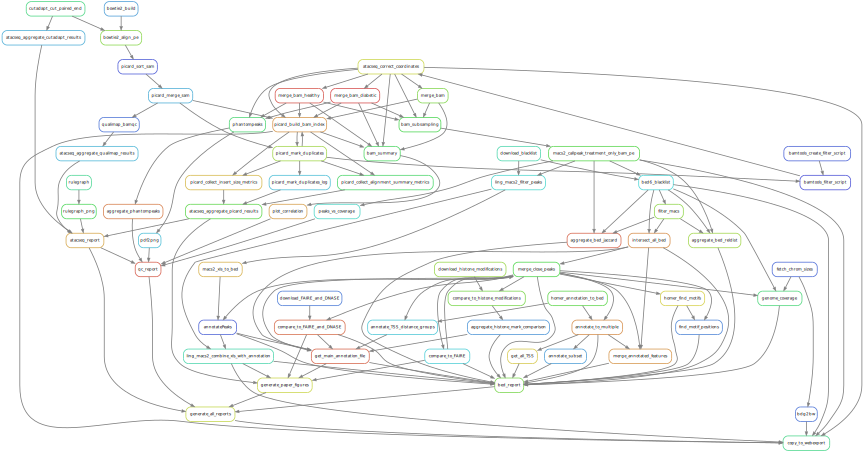
\includegraphics[height=.7\paperheight]{example_dags/rulegraph_complex.png}\hfil}\vfil}
	}
	\frame{
		\frametitle{Selecting Workflows}
		\begin{mdframed}[tikzsetting={draw=white,fill=white,fill opacity=0.8,
				line width=0pt},backgroundcolor=none,leftmargin=0,
			rightmargin=150,innertopmargin=4pt,roundcorner=10pt]
			\tableofcontents[currentsection,sections={1-4},hideothersubsections]
		\end{mdframed}
	}
}


%%%%%%%%%%%%%%%%%%%%%%%%%%%%%%%%%%%%%%%%%%%%%%%%%%%%%%%%%%%%%%%%%%%%%%%%%%%%%%%%
\begin{frame}
  \frametitle{What is this about?}
   \begin{question}[Questions]
   	 \begin{itemize}
       \item How do I get a workflow for a given scientific problem?
       \item How do I run such an arbitrary workflow?
     \end{itemize}
   \end{question} 
   \begin{docs}[Objectives]
   	  \begin{enumerate}
                      \item Introducing the workflow catalogue!
                      \item Learning the difference between ``curation'' (what some people think) and ``curation'' (what really works).
      \end{enumerate}
    \end{docs}
\end{frame}  

\subsection{The Snakemake Workflow Catalogue}

%%%%%%%%%%%%%%%%%%%%%%%%%%%%%%%%%%%%%%%%%%%%%%%%%%%%%%%%%%%%%%%%%%%%%%%%%%%%%%%
\begin{frame}
 \frametitle{Selecting and Downloading from the Workflow Catalogue}
 You can find the \Snakemake{} worfkflow catalogue, \lhref{https://snakemake.github.io/snakemake-workflow-catalog/?rules=true}{here}. It makes a difference between workflows which meet best-practice criteria - and those which do not.\newline
 \begin{columns}
   \begin{column}{0.5\textwidth}
     You can download and run any workflow. \Snakemake's portability features ensure it will work everywhere $\ldots$\pause
     \begin{warning}
     	$\ldots$ except, you most likely cannot, because of a missing cluster configuration.
     \end{warning}
   \end{column}
   \begin{column}{0.5\textwidth}
     \includegraphics[width=\textwidth]{Snakemake/Snakemake_Workflow_Catalog.png}
   \end{column}
 \end{columns}
\end{frame}

%%%%%%%%%%%%%%%%%%%%%%%%%%%%%%%%%%%%%%%%%%%%%%%%%%%%%%%%%%%%%%%%%%%%%%%%%%%%%%%
\begin{frame}
  \frametitle{Searching \emph{your} Workflow}
   \begin{columns}
  	\begin{column}{0.5\textwidth}
  		\includegraphics[width=\textwidth]{Snakemake/Searching_Workflows_in_Catalog.png}
  	\end{column}
  	\begin{column}{0.5\textwidth}
  		You can look for 
  		\begin{itemize}
  		  \item topical keywords and
  		  \item software
  		\end{itemize}
  	\end{column}
  \end{columns}
\end{frame}

%%%%%%%%%%%%%%%%%%%%%%%%%%%%%%%%%%%%%%%%%%%%%%%%%%%%%%%%%%%%%%%%%%%%%%%%%%%%%%%
\begin{frame}
	\frametitle{Workflows Compliance}
	\begin{question}[Noted this?]
	  \includegraphics[width=0.8\textwidth]{Snakemake/Snakemake_Workflow_Catalog_Categories.png}
	\end{question}
\end{frame}

%%%%%%%%%%%%%%%%%%%%%%%%%%%%%%%%%%%%%%%%%%%%%%%%%%%%%%%%%%%%%%%%%%%%%%%%%%%%%%%%
\begin{frame}[fragile]
  \frametitle{Deployment}
  Select (=click on) any desired workflow. There are three alternatives:
  \begin{enumerate}[<+->]
   \item a workflow offers a release - in which case you can download and unpack it
   \item all workflows offers a ``\altverb{git clone}'' hint
   \item or you use the \altverb{snakedeploy} to get everything you need.
  \end{enumerate}
\end{frame}

%%%%%%%%%%%%%%%%%%%%%%%%%%%%%%%%%%%%%%%%%%%%%%%%%%%%%%%%%%%%%%%%%%%%%%%%%%%%%%%%
\begin{frame}[fragile]
	\frametitle{Deployment II - Creating an Environment Fork}
	Usually, we can create an environment like:
	\begin{lstlisting}[language=Bash, style=Shell]
$ mamba create -c conda-forge -c bioconda -n snakemake \
> snakemake snakemake-executor-plugin-slurm \
> snakemake-storage-plugin-fs
    \end{lstlisting}
    This should install a \Snakemake{} environment with all necessary tools!
\end{frame}

%%%%%%%%%%%%%%%%%%%%%%%%%%%%%%%%%%%%%%%%%%%%%%%%%%%%%%%%%%%%%%%%%%%%%%%%%%%%%%%%
\begin{frame}[fragile]
	\frametitle{Deployment III - First Step!}
	Follow step 2 of a selected workflow usage instructions:
	\begin{columns}
		\begin{column}{0.4\textwidth}
			\centering
			\includegraphics[width=0.95\textwidth]{Snakemake/deploy_workflow}
		\end{column}
	    \begin{column}{0.6\textwidth}
	    	A usual command is:
	    	\begin{lstlisting}[language=Bash, style=Shell]
$ snakedeploy deploy-workflow \
> <URL>
	    	\end{lstlisting}
    	    This will create the directories \altverb{workflow} and \altverb{config} in your current directory.
    	    \begin{hint}
    	    	Alternatively, you may navigate to the repository of your desired workflow and download the entire workflow.
    	    \end{hint}
	    \end{column}
	\end{columns}
\end{frame}

%%%%%%%%%%%%%%%%%%%%%%%%%%%%%%%%%%%%%%%%%%%%%%%%%%%%%%%%%%%%%%%%%%%%%%%%%%%%%%%%
\begin{frame}[fragile]
	\frametitle{Finalizing the Deploymment}

		We could now deploy our sample workflow:
		\begin{itemize}
			\item Please create a directory \altverb{mkdir -p ~/example_workflow}
			\item Change to this directory.
			\item Deploy our sample workflow with
		\end{itemize}
        \begin{lstlisting}[language=Bash, style=Shell]
$ snakedeploy deploy-workflow \
> <++course.deploy_url++>
       \end{lstlisting}
\end{frame}


%%%%%%%%%%%%%%%%%%%%%%%%%%%%%%%%%%%%%%%%%%%%%%%%%%%%%%%%%%%%%%%%%%%%%%%%%%%%%%%%
\begin{frame}[fragile]
  \frametitle{Running Workflows on Cluster (or other environment)}
  Most likely a specific workflow never has been testing on \emph{your} computer before. It is almost ensured it will run on arbitrary servers, but clusters are a different story. \newline
  So
  \begin{itemize}[<+->]
   \item try to parameterize your workflow as we will learn and create a "profile"
   \item if it gives issues and you know how to correct it, ``fork'' the worklow and create a pull request
   \item if you cannot fix it, create a bug report
  \end{itemize}
\end{frame}

%%%%%%%%%%%%%%%%%%%%%%%%%%%%%%%%%%%%%%%%%%%%%%%%%%%%%%%%%%%%%%%%%%%%%%%%%%%%%%%%
\begin{frame}
  \frametitle{\Interlude{Learn git!}}
  If you do not know what ``fork'' and ``pull request'' means, learn git!
  \begin{itemize}[<+->]
   \item there are courses
   \item and lots of online material
   \item and books
  \end{itemize}
  \pause
  \begin{warning}
  	Knowing git is essential in data analysis!
  \end{warning}
\end{frame}

%%%%%%%%%%%%%%%%%%%%%%%%%%%%%%%%%%%%%%%%%%%%%%%%%%%%%%%%%%%%%%%%%%%%%%%%%%%%%%%%
\begin{frame}[fragile]
  \frametitle{\HandsOn{Configuring the Workflow}}
  It is now time to configure and parameterize the workflow.
  \pause
  \begin{hint}
  	As the configuration is workflow dependent you need to follow instructions, now.
  \end{hint}
  \pause
  Eventually start the workflow using:
  \begin{lstlisting}[language=Bash, style=Shell]
$ snakemake --executor slurm \
> -j unlimited \
> --configfile <path to file> \
> --workflow-profile <path to directory> \
> --directory <path to your course output>
  \end{lstlisting}
  \pause
  \begin{hint}
  	We will learn a few tricks to shorten this line.
  \end{hint}
\end{frame}



%%%%%%%%%%%%%%%%%%%%%%%%%%%%%%%%%%%%%%%%%%%%%%%%%%%%%%%%%%%%%%%%%%%%%%%%%%%%%%%%
% \include{common/Using_Workflow_Configs}

%%%%%%%%%%%%%%%%%%%%%%%%%%%%%%%%%%%%%%%%%%%%%%%%%%%%%%%%%%%%%%%%%%%%%%%%%%%%%%%%
%%%%%%%%%%%%%%%%%%%%%%%%%%%%%%%%%%%%%%%%%%%%%%%%%%%%%%%%%%%%%%%%%%%%%%%%%%%%%%%%
\section{Plotting DAGs}
{   
	\usebackgroundtemplate{
		\vbox to \paperheight{\vfil\hbox to \paperwidth{\hfil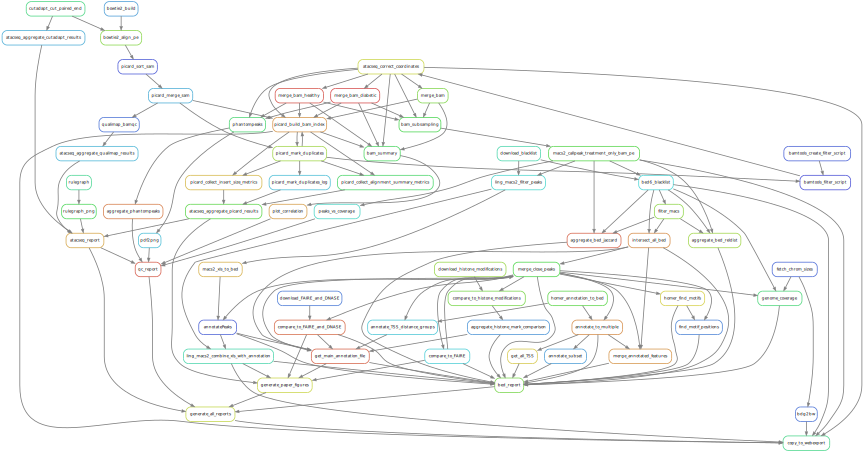
\includegraphics[height=\paperheight]{example_dags/rulegraph_complex.png}\hfil}\vfil}
		% source: https://en.m.wikipedia.org/wiki/File:Text-x-python.svg
	}
	\frame{
		\frametitle{Plotting Workflow Graphs}
		\begin{mdframed}[tikzsetting={draw=white,fill=white,fill opacity=0.8,
				line width=0pt},backgroundcolor=none,leftmargin=0,
			rightmargin=150,innertopmargin=4pt,roundcorner=10pt]
			\tableofcontents[currentsection,sections={1-4},hideothersubsections]
		\end{mdframed}
	}
}

%%%%%%%%%%%%%%%%%%%%%%%%%%%%%%%%%%%%%%%%%%%%%%%%%%%%%%%%%%%%%%%%%%%%%%%%%%%%%%%%
\begin{frame}
  \frametitle{What is this about?}
   \begin{question}[Questions]
   	 \begin{itemize}
       \item How do we plot our workflows for a publication?
     \end{itemize}
   \end{question}
   \begin{docs}[Objectives]
   	  \begin{enumerate} 
                      \item Learn to plot workflows using \Snakemake{} and GraphViz.
      \end{enumerate}
   \end{docs}
\end{frame}

%%%%%%%%%%%%%%%%%%%%%%%%%%%%%%%%%%%%%%%%%%%%%%%%%%%%%%%%%%%%%%%%%%%%%%%%%%%%%%%%
\begin{frame}[fragile]
  \frametitle{\HandsOn{Plotting the Workflow}}
  \Snakemake{} has a build-in plotting feature. Run 
  \begin{lstlisting}[language=Bash, style=Shell]
$ snakemake --rulegraph | dot -Tpng > <your_workflow.png>
  \end{lstlisting}
  to plot your workflow graph. And
  \begin{lstlisting}[language=Bash, style=Shell]
$ display <your_workflow.png>
  \end{lstlisting}
  to display the workflow.
\end{frame}

%%%%%%%%%%%%%%%%%%%%%%%%%%%%%%%%%%%%%%%%%%%%%%%%%%%%%%%%%%%%%%%%%%%%%%%%%%%%%%%%
\begin{frame}
  \frametitle{Your DAG:}
  \centering
  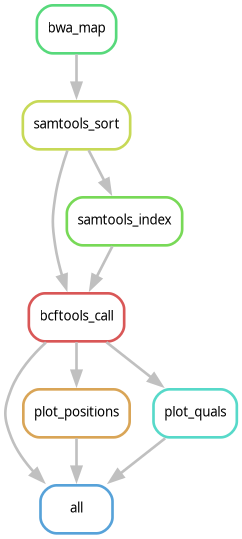
\includegraphics[height=0.5\textheight]{workflows/rulegraph_lifescience.png}
\end{frame}

%%%%%%%%%%%%%%%%%%%%%%%%%%%%%%%%%%%%%%%%%%%%%%%%%%%%%%%%%%%%%%%%%%%%%%%%%%%%%%%%
\begin{frame}[fragile]
  \frametitle{\HandsOn{Produce different Plots}}
  What do you observe, if you try:
  \begin{lstlisting}[language=Bash, style=Shell,basicstyle=\footnotesize]
$ snakemake --rulegraph | dot -Tpng > <your_rulegraph.png>
$ # or
$ snakemake --filegraph | dot -Tpng > <your_filegraph.png>
$ # or
$ snakemake --dag | dot -Tpng > <your_dag.png>
$ # or --dag again after
$ snakemake --delete-all-output -c1
  \end{lstlisting}
\end{frame}

%%%%%%%%%%%%%%%%%%%%%%%%%%%%%%%%%%%%%%%%%%%%%%%%%%%%%%%%%%%%%%%%%%%%%%%%%%%%%%%%
\begin{frame}[fragile]
 \frametitle{Plot Comparison}
 \begin{figure}
  \centering
  \subfloat[\centering \altverb{--rulegraph}]{{ 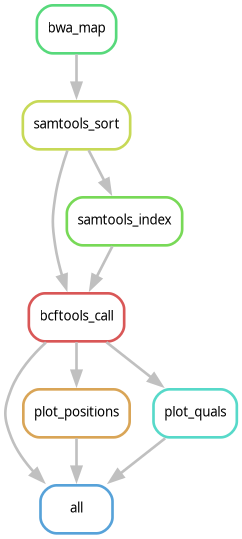
\includegraphics[width=0.2\textwidth, height=0.5\textheight]{workflows/rulegraph_lifescience.png} }}
  \subfloat[\centering \altverb{--filegraph}]{{ 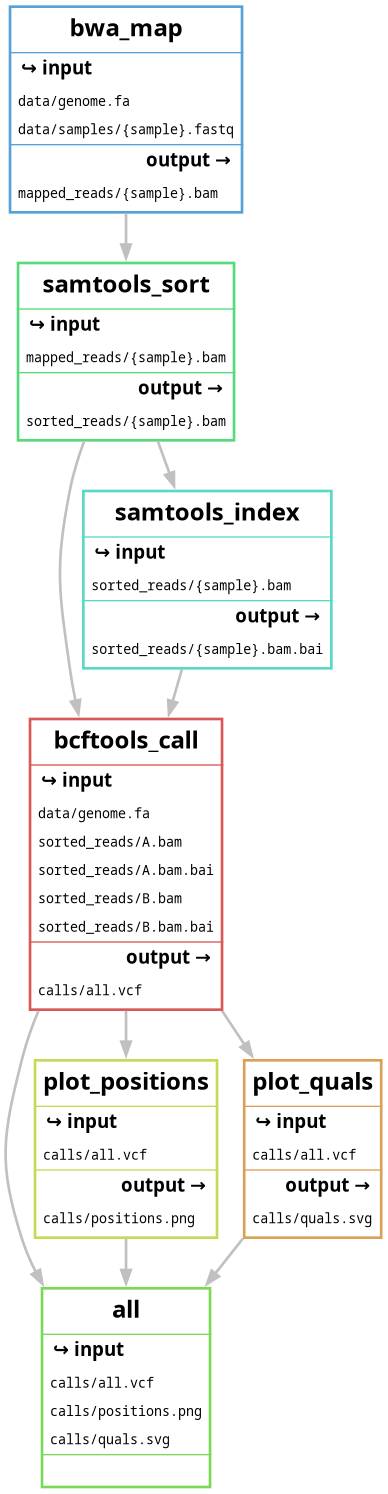
\includegraphics[width=0.2\textwidth, height=0.5\textheight]{workflows/filegraph_lifescience.png} }}
  \subfloat[\centering \altverb{--dag}, with rules done]{{ 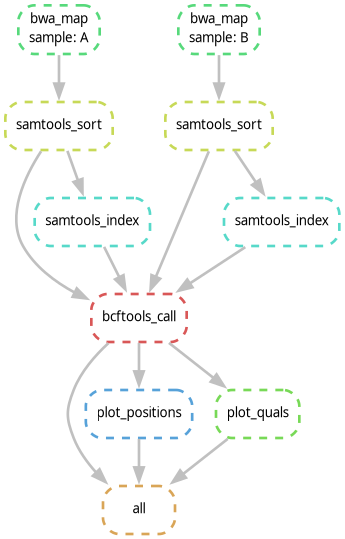
\includegraphics[width=0.2\textwidth, height=0.5\textheight]{workflows/dag_lifescience.png} }}
  \subfloat[\centering \altverb{--dag}, with rules still to do]{{ 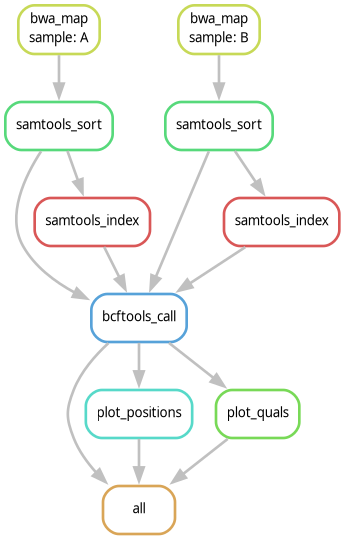
\includegraphics[width=0.2\textwidth, height=0.5\textheight]{workflows/dag_full_lifescience.png} }}
\end{figure}

\end{frame}






%%%%%%%%%%%%%%%%%%%%%%%%%%%%%%%%%%%%%%%%%%%%%%%%%%%%%%%%%%%%%%%%%%%%%%%%%%%%%%%%
%%%%%%%%%%%%%%%%%%%%%%%%%%%%%%%%%%%%%%%%%%%%%%%%%%%%%%%%%%%%%%%%%%%%%%%%%%%%%%%%
\section{How does Clustercomputing work?}
{   
	\usebackgroundtemplate{
		\vbox to \paperheight{\vfil\hbox to \paperwidth{\hfil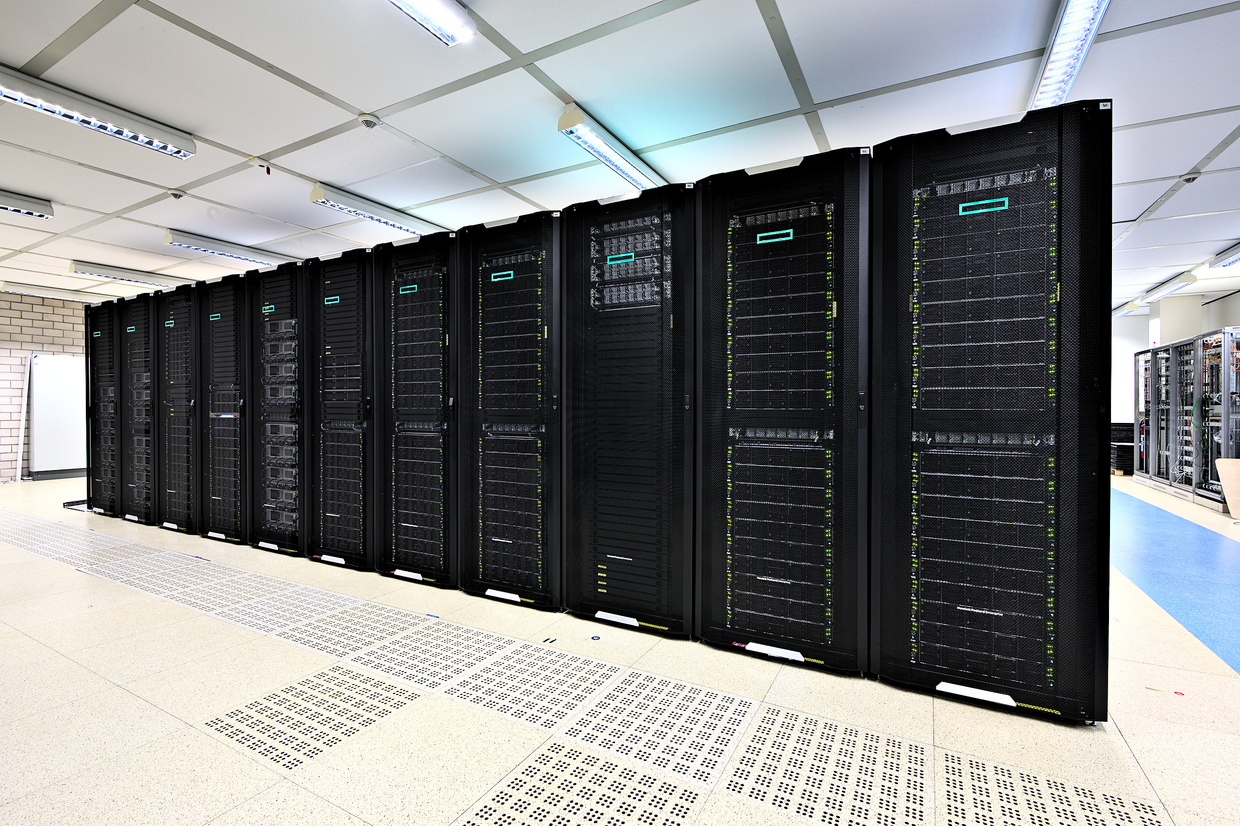
\includegraphics[height=\paperheight]{misc/cluster_kit}\hfil}\vfil}
		% source: https://en.m.wikipedia.org/wiki/File:Text-x-python.svg
	}
	\frame{
		\frametitle{Running ordinary Batch Scripts}
		\begin{mdframed}[tikzsetting={draw=white,fill=white,fill opacity=0.8,
				line width=0pt},backgroundcolor=none,leftmargin=0,
			rightmargin=150,innertopmargin=4pt,roundcorner=10pt]
			\tableofcontents[currentsection,sections={1-4},hideothersubsections]
		\end{mdframed}
	}
}


%%%%%%%%%%%%%%%%%%%%%%%%%%%%%%%%%%%%%%%%%%%%%%%%%%%%%%%%%%%%%%%%%%%%%%%%%%%%%%%%
\begin{frame}
  \frametitle{What is this about?}
    \begin{question}
   	  \begin{itemize}
        \item How does ordinary job submission work on a cluster?
        \item How does it work using Snakemake? (Which parameterization is necessary?)
      \end{itemize}
   \end{question}
   \begin{docs}[Objectives]
   	 \begin{enumerate}
   	 	\item Get a feeling for the SLURM batch system.
   	 	\item We want to give you an idea of building a workflow with \emph{pure} batch system commands, first.
     \end{enumerate}
   \end{docs}
\end{frame}


%%%%%%%%%%%%%%%%%%%%%%%%%%%%%%%%%%%%%%%%%%%%%%%%%%%%%%%%%%%%%%%%%%%%%%%%%%%%%%%%
\subsection*{The \slurm Scheduler}

%%%%%%%%%%%%%%%%%%%%%%%%%%%%%%%%%%%%%%%%%%%%%%%%%%%%%%%%%%%%%%%%%%%%%%%%%%%%%%%% 
\begin{frame}
  \frametitle{What is a scheduler?}
  On HPC systems you do not \emph{just start}, you need a \emph{``scheduler''}.
  So, what's that?\newline
  A scheduler (or ``batch system'') on a HPC system should\ldots
  \begin{itemize}
  \item provide an interface to help defining workflows and/or job dependencies
  \item enable automatic submission of executions
  \item provide interfaces to monitor the executions
  \item prioritise the execution order of unrelated jobs
  \end{itemize}
  \begin{columns}
    \begin{column}{0.8\linewidth}
      This is an micro-intro to the \slurm batch system.
    \end{column}
    \begin{column}{0.2\linewidth}
      \begin{figure}
        \centering
        \includegraphics[height=1.5cm,width=1.5cm]{logos/slurm_logo.png}
      \end{figure}
    \end{column}
  \end{columns}
  \vfill
\end{frame}

%%%%%%%%%%%%%%%%%%%%%%%%%%%%%%%%%%%%%%%%%%%%%%%%%%%%%%%%%%%%%%%%%%%%%%%%%%%%%%%% 
\begin{frame}
  \frametitle{Promises, promises and even more promises}
  How does a scheduler work?
  \pause
  \begin{block}{You tell it\ldots}
    \begin{itemize}
    \item how much memory (RAM, scratch space) your job will need.\pause
    \item how much time you will spend on it.\pause
    \item how many CPUs you will need (and in which combination).\pause
    \item whether you need something special (e.g. a GPU).
    \end{itemize}
  \end{block}
  \pause \vspace{-0.2cm}
  \begin{exampleblock}{The scheduler will act:}
    \begin{itemize}
    \item It will queue up your job (and decide when it will start relative to others).\pause
    \item It will decide where your job will run physically (which hosts).\pause
    \item Eventually it will start your job (if everything was correct).
    \end{itemize}
  \end{exampleblock}
  \vfill
\end{frame}

\setcounter{preframe_handson}{\value{handson}}
%%%%%%%%%%%%%%%%%%%%%%%%%%%%%%%%%%%%%%%%%%%%%%%%%%%%%%%%%%%%%%%%%%%%%%%%%%%%%%%% 
\begin{frame}[fragile]
  \setcounter{handson}{\value{preframe_handson}}
  \frametitle{\HandsOn{Your first job script}}
  \begin{hint}
  	    From now on, we will be scripting examples (cloze-based). For this you will
        need an editor. If you do not know any other editor, use \texttt{gedit}:
  \end{hint}
  \begin{lstlisting}[language=Bash, style=Shell, basicstyle=\scriptsize]
$ # cd into appropriate directory
$ # Start gedit with the command 
$ gedit &
  \end{lstlisting}
  \begin{hint}
  	The \texttt{\&} will put the editor into the background.
  \end{hint} 
\end{frame}

%%%%%%%%%%%%%%%%%%%%%%%%%%%%%%%%%%%%%%%%%%%%%%%%%%%%%%%%%%%%%%%%%%%%%%%%%%%%%%% 
\input{<++course.hello_world_script++>}

%%%%%%%%%%%%%%%%%%%%%%%%%%%%%%%%%%%%%%%%%%%%%%%%%%%%%%%%%%%%%%%%%%%%%%%%%%%%%%%% 
\begin{frame}[fragile]%
	\frametitle{Please Imaging \ldots}
	Now, thing of your analysis workflow: QC, preprocessing, processing, analysis, post-processing and plotting and \ldots \newline
	\pause
	All this \emph{can} be achieved with SLURM, too all with bash:
	\begin{lstlisting}[language=Bash, style=Shell]
# First, do some pre-processing for the first job.
...
# Then, submit a job without dependencies.
jid1=$(sbatch ... job1.sh)
# NOTE: ALL 'job*sh' scripts are bash scripts,
#       with more logic than the "hello world" script.		

# Next, do some more logic as pre-processing for the 
# follow-up jobs. ...
# multiple jobs can depend on a single job
jid2=$(sbatch --dependency=afterany:$jid1 ... job2.sh)
jid3=$(sbatch --dependency=afterany:$jid1 ... job3.sh)
	\end{lstlisting}
    etc. can easily be a few thousand lines for \emph{every} workflow.
	\vfill
\end{frame}


%%%%%%%%%%%%%%%%%%%%%%%%%%%%%%%%%%%%%%%%%%%%%%%%%%%%%%%%%%%%%%%%%%%%%%%%%%%%%%%% 
\begin{frame}
  \frametitle{End of HPC Intro}
  We could co on with \emph{many} details with regards to the scheduler, the file system, etc..
  \begin{block}{HPC Courses}
   HPC teams offers courses to:
   \begin{itemize}
    \item HPC Intro
    \item Bash Intro
    \item Research Data Management
    \item many other topics
   \end{itemize}
  \end{block}
  \pause
  \begin{hint}[What's next]
      We are going to parameterize our workflow\textbf{s} for clusters and for our applications in \Snakemake!
  \end{hint}
\end{frame}







%%%%%%%%%%%%%%%%%%%%%%%%%%%%%%%%%%%%%%%%%%%%%%%%%%%%%%%%%%%%%%%%%%%%%%%%%%%%%%%%
%%%%%%%%%%%%%%%%%%%%%%%%%%%%%%%%%%%%%%%%%%%%%%%%%%%%%%%%%%%%%%%%%%%%%%%%%%%%%%%%
\section{Parameterizing your Workflow (II) - I/O}
{   
	\usebackgroundtemplate{
		\vbox to \paperheight{\vfil\hbox to \paperwidth{\hfil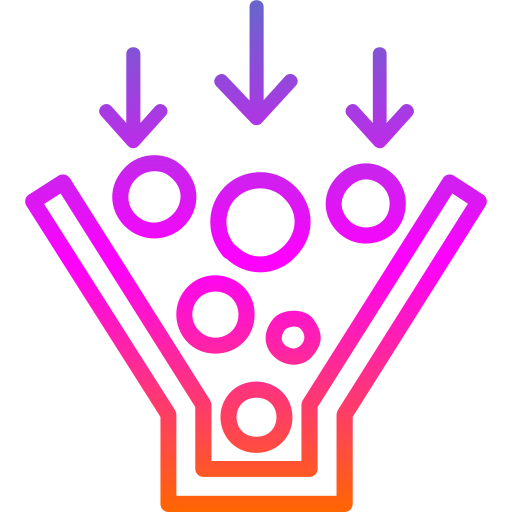
\includegraphics[height=\paperheight]{misc/bottleneck.png}\hfil}\vfil}
	}
	\frame{
		\frametitle{Avoiding I/O Contention}
		\begin{mdframed}[tikzsetting={draw=white,fill=white,fill opacity=0.8,
				line width=0pt},backgroundcolor=none,leftmargin=0,
			rightmargin=150,innertopmargin=4pt,roundcorner=10pt]
			\tableofcontents[currentsection,sections={1-4},hideothersubsections]
			\vspace{1em}
			\tiny \lhref{https://www.flaticon.com/free-icon/bottleneck_10803803}{from Flaticon}
		\end{mdframed}
	}
}
%%%%%%%%%%%%%%%%%%%%%%%%%%%%%%%%%%%%%%%%%%%%%%%%%%%%%%%%%%%%%%%%%%%%%%%%%%%%%%%%
\begin{frame}
  \frametitle{What is this about?}
  \begin{question}[Questions]
   	\begin{itemize}
      \item How do we avoid I/O contention?
      \item How do we account for file system latency?
    \end{itemize}
  \end{question}
   \begin{docs}[Objectives]
   	 \begin{enumerate} 
        \item Learn how to tune \Snakemake{} to mitigate I/O contention.
        \item Learn how to configure \Snakemake{} to allow for file system latency.
    \end{enumerate}
  \end{docs}
\end{frame}

%%%%%%%%%%%%%%%%%%%%%%%%%%%%%%%%%%%%%%%%%%%%%%%%%%%%%%%%%%%%%%%%%%%%%%%%%%%%%%%%
\begin{frame}
	\frametitle{\Interlude{What is Random Access?}}
	\vspace{-1.5em}
	\begin{figure}
		\centering
		\begin{tikzpicture}
			\node[name=sa] at (3.5,10) { \lhref{https://en.wikipedia.org/wiki/Random_access}{Sequential Access} };
			\foreach[count=\y from 2] \x in {1,...,11}{
				\draw[thick,black,midway,draw] (\x,8.75) rectangle node[name=s\x] {} (\y,8.25);
			}       
			\foreach[count=\y from 2] \x in  {1, ..., 10} {
					\path[->] ([yshift=.6em]s\x.north west) edge[bend left=30] ([yshift=.6em]s\y.north west);
			}
			%         \path[->] ([yshift=.6em]s1.north) edge [bend left=30] ([yshift=.6em]s2.north) ;
			
			\node[name=ra] at (3.5,7) { Random Access };
			\foreach[count=\y from 2] \x in {1,...,11}{
				\draw[thick,black,midway,draw] (\x,5.75) rectangle node[name=r\x] {} (\y,5.25);
			}
		
			\path[->] ([yshift=.6em]r1.north) edge [bend left=30] ([yshift=.6em]r5.north) ;
			\path[->] ([yshift=.6em]r5.north) edge [bend right=60] ([yshift=.6em]r2.north) ;
			\path[->] ([yshift=.6em]r2.north) edge [bend left=30] ([yshift=.6em]r3.north) ;
			\path[->] ([yshift=.6em]r3.north) edge [bend left=30] ([yshift=.6em]r11.north) ;
			\path[->] ([yshift=.6em]r11.north) edge [bend right=30] ([yshift=.6em]r7.north) ;
			\path[->] ([yshift=.6em]r7.north) edge [bend right=30] ([yshift=.6em]r6.north) ;
			\path[->] ([yshift=.6em]r6.north) edge [bend left=60] ([yshift=.6em]r8.north) ;
			\path[->] ([yshift=.6em]r8.north) edge [bend right=50] ([yshift=.6em]r4.north) ;
		\end{tikzpicture}
	\end{figure}
\end{frame}

%%%%%%%%%%%%%%%%%%%%%%%%%%%%%%%%%%%%%%%%%%%%%%%%%%%%%%%%%%%%%%%%%%%%%%%%%%%%%%%%
\begin{frame}
	\frametitle{\Interlude{What is Random Access?}}
	\begin{question}
	  \begin{itemize}
	  	\item What causes Random Access?
	  	\item Why is it harmful? What can we do?
	  \end{itemize}
    \end{question}
	\pause
	\begin{columns}[t]
	  \begin{column}{0.5\textwidth}
	  	Causes:
	  	\hrule
	  	\begin{itemize}
	  	  \item a number of (threaded) apps accessing the same file space (e.g. reference data)
	  	  \item a number of apps accessing a file space exceeding the file system cache size
	  	\end{itemize}
  	     Will slow parallel file systems and your data analysis!
	  \end{column}
      \begin{column}{0.5\textwidth}
      	Remedies:
      	\hrule
      	\begin{itemize}
      		\item copy data to/from compute nodes equipped with SSD
      		\item use a RAM disk (RAM = random access memory) - which many clusters provide
      	\end{itemize}
      \end{column}
	\end{columns}	
\end{frame}

%%%%%%%%%%%%%%%%%%%%%%%%%%%%%%%%%%%%%%%%%%%%%%%%%%%%%%%%%%%%%%%%%%%%%%%%%%%%%%%%
\begin{frame}
  \frametitle{\Interlude{What is File System Latency?}}
    \centering
	\begin{tikzpicture}[line cap=rect,line width=3pt, 
		datastore/.style={draw, rounded rectangle, rounded rectangle east arc=concave, rounded rectangle arc length=150},
		]
	  \tikzstyle{storage} = [rectangle, minimum width=3cm, minimum height=1cm, text width=3cm, text centered, draw=black]
	  
	  \filldraw [fill=cyan] (0,0) circle [radius=1cm];
	  \foreach \angle [count=\xi] in {60,30,...,-270}
	  {
		\draw[line width=0.5pt] (\angle:0.9cm) -- (\angle:1cm);
		\node[font=\small] at (\angle:0.68cm) {\textsf{\xi}};
	  }
	  \foreach \angle in {0,90,180,270}
	  \draw[line width=1pt] (\angle:0.8cm) -- (\angle:1cm);
	  \draw (0,0) -- (120:0.4cm);
	  \draw (0,0) -- (90:.5cm);
	  
	  \node (sto1) [datastore] at (-4, 0) {Storage};
	  \node at (4, 0) {\includegraphics[width=.25\textwidth]{misc/data_center.png}};
  \end{tikzpicture}
  \begin{docs}{File System Latency}
  	The time it takes from the file system to the client and back.
  \end{docs}
\end{frame}

%%%%%%%%%%%%%%%%%%%%%%%%%%%%%%%%%%%%%%%%%%%%%%%%%%%%%%%%%%%%%%%%%%%%%%%%%%%%%%%%
\begin{frame}
  \frametitle{\Interlude{What is File System Latency? II}}
  \begin{docs}{Background}
  	Some clusters use NFS (Network File System). There, file system latency \emph{can} be an issue.\newline
  	\pause
  	On parallel file systems, the latency usually is very low. 
  \end{docs}	
\end{frame}


%%%%%%%%%%%%%%%%%%%%%%%%%%%%%%%%%%%%%%%%%%%%%%%%%%%%%%%%%%%%%%%%%%%%%%%%%%%%%%%%
\subsection{Global Workflow Configuration}

%%%%%%%%%%%%%%%%%%%%%%%%%%%%%%%%%%%%%%%%%%%%%%%%%%%%%%%%%%%%%%%%%%%%%%%%%%%%%%%%
\begin{frame}[fragile]
  \frametitle{\Snakemake{} Profiles}
  \begin{hint}
  	Profiles can shorten your command lines and be an easy remedy for the described issues!
  \end{hint}
  \pause
  Two kinds of profiles are supported:
  \begin{itemize}[<+->]
  	\item A global profile that is defined in a system-wide or user-specific configuration directory (on Linux, this will be \altverb{\~/.config/snakemake} and \altverb{/etc/xdg/snakemake}, you can find the answer for your system via \altverb{snakemake --help}).
  	\item A workflow specific profile that is defined via a flag (\altverb{--workflow-profile}) or searched in a default location (profile/default) in the working directory or next to the \altverb{Snakefile}.
  \end{itemize}
\end{frame}

%%%%%%%%%%%%%%%%%%%%%%%%%%%%%%%%%%%%%%%%%%%%%%%%%%%%%%%%%%%%%%%%%%%%%%%%%%%%%%%%
\begin{frame}[fragile]
  \frametitle{Your Profile}
    \begin{onlyenv}<1| handout:0>
      Your first line forces the executor to be set to \slurm - persistently.
      \begin{lstlisting}[language=Bash, style=Shell]
executor: slurm
     \end{lstlisting}
     No more, \altverb{snakemake --executor slurm ...}!
   \end{onlyenv}
   \begin{onlyenv}<2| handout:0>
   	 The next line tells \Snakemake to wait for 5 seconds, if output files are not present (because we are working with parallel file systems). 
   	 \begin{lstlisting}[language=Bash, style=Shell]
executor: slurm
latency-wait: 5
   	 \end{lstlisting}
    \end{onlyenv}
    \begin{onlyenv}<3| handout:0>
      The entire rest, will tell the storage plugin (\altverb{snakemake-storage-plugin-fs}) to stage in to the node-local storage on your cluster, for \emph{every} job and to copy back your results. When dealing with I/O intensive jobs, this can boost your performance tremendously. 
      \begin{lstlisting}[language=Bash, style=Shell]
executor: slurm
latency-wait: 5
default-storage-provider: fs
shared-fs-usage:
  - persistence
  - sources
  - source-cache
remote-job-local-storage-prefix: |
    <++cluster.remotejoblocalstorageprefix++>
local-storage-prefix: <++cluster.localstorageprefix++>
    \end{lstlisting}
   \end{onlyenv}
   \begin{onlyenv}<4| handout:1>
   	The complete configuration out to be in \altverb{\~/.config/snakemake/config.yaml}
   	\begin{lstlisting}[language=Bash, style=Shell]
executor: slurm
latency-wait: 5
default-storage-provider: fs
shared-fs-usage:
  - persistence
  - sources
  - source-cache
remote-job-local-storage-prefix: |
     <++cluster.remotejoblocalstorageprefix++>
local-storage-prefix: <++cluster.localstorageprefix++>
    \end{lstlisting}
  \end{onlyenv}
\end{frame}


%%%%%%%%%%%%%%%%%%%%%%%%%%%%%%%%%%%%%%%%%%%%%%%%%%%%%%%%%%%%%%%%%%%%%%%%%%%%%%%%
\begin{frame}[fragile]
	\frametitle{\HandsOn{Running with a Profile I}}
	Enter 
	\begin{lstlisting}[language=Bash, style=Shell]
export SNAKEMAKE_PROFILE="$HOME/.config/snakemake"
    \end{lstlisting}
	in your \altverb{.bashrc}
\end{frame}

%%%%%%%%%%%%%%%%%%%%%%%%%%%%%%%%%%%%%%%%%%%%%%%%%%%%%%%%%%%%%%%%%%%%%%%%%%%%%%%%
\begin{frame}[fragile]
	\frametitle{\HandsOn{Running with a Profile II}}
	Copy the configuration file:
	\begin{lstlisting}[language=Bash, style=Shell]
$ mkdir -p ~/.config/snakemake
$ cp ~/workflows/config.yaml \
> ~/.config/snakemake/.
	\end{lstlisting}
    Activate the new settings:
    \begin{lstlisting}[language=Bash, style=Shell]
$ source ~/.bashrc
    \end{lstlisting}
    And run the workflow - just for fun:
    \begin{lstlisting}[language=Bash, style=Shell]
$ snakemake -F # just this one flag!
    \end{lstlisting}
\end{frame}

	


      
%%%%%%%%%%%%%%%%%%%%%%%%%%%%%%%%%%%%%%%%%%%%%%%%%%%%%%%%%%%%%%%%%%%%%%%%%%%%%%%%
\include{common/Reports}    

%%%%%%%%%%%%%%%%%%%%%%%%%%%%%%%%%%%%%%%%%%%%%%%%%%%%%%%%%%%%%%%%%%%%%%%%%%%%%%%%
%%%%%%%%%%%%%%%%%%%%%%%%%%%%%%%%%%%%%%%%%%%%%%%%%%%%%%%%%%%%%%%%%%%%%%%%%%%%%%%%%
\section{Snakemake Wrappers}
{   
	\usebackgroundtemplate{
		\vbox to \paperheight{\vfil\hbox to \paperwidth{\hfil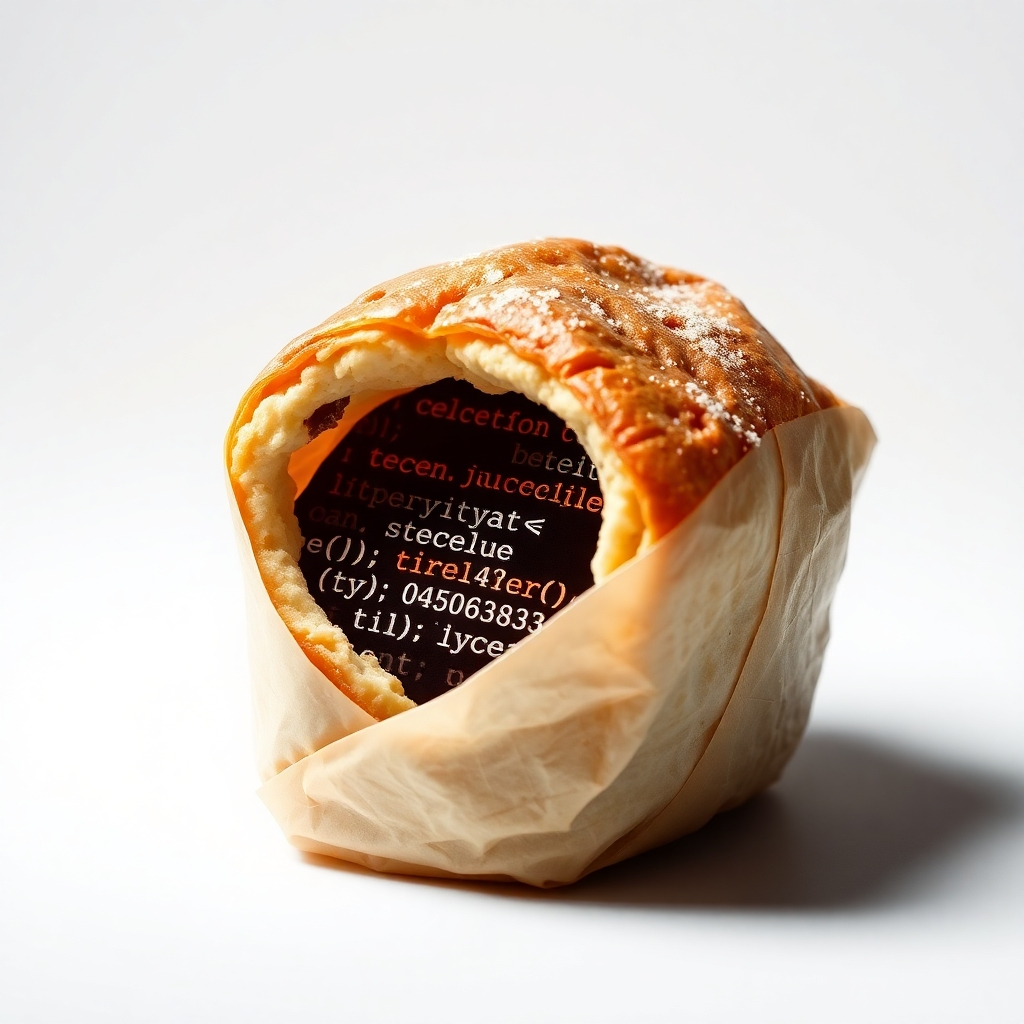
\includegraphics[height=.7\paperheight]{misc/wrapper.jpg}\hfil}\vfil}
	}
	\frame{
		\frametitle{Using \Snakemake-Wrappers}
		\begin{mdframed}[tikzsetting={draw=white,fill=white,fill opacity=0.8,
				line width=0pt},backgroundcolor=none,leftmargin=0,
			rightmargin=150,innertopmargin=4pt,roundcorner=10pt]
			\tableofcontents[currentsection,sections={1-4},hideothersubsections]
		\end{mdframed}
	}
}

%%%%%%%%%%%%%%%%%%%%%%%%%%%%%%%%%%%%%%%%%%%%%%%%%%%%%%%%%%%%%%%%%%%%%%%%%%%%%%%%
\subsection{Using Wrappers}

%%%%%%%%%%%%%%%%%%%%%%%%%%%%%%%%%%%%%%%%%%%%%%%%%%%%%%%%%%%%%%%%%%%%%%%%%%%%%%%%
\begin{frame}
    \frametitle{What is this about?}
    \begin{question}[Questions]
        \begin{itemize}
            \item What is a \Snakemake{} Wrapper?
            \item How can \Snakemake{} wrappers be used to write reproducible workflows?
        \end{itemize}
    \end{question}
    \begin{docs}[Objectives]
        \begin{enumerate}
            \item Introduce the concept of \Snakemake{} wrappers
            \item Include \Snakemake{} wrappers in your workflows
            \item Reproducibility of \Snakemake{} wrappers
        \end{enumerate}
    \end{docs}
\end{frame}

%%%%%%%%%%%%%%%%%%%%%%%%%%%%%%%%%%%%%%%%%%%%%%%%%%%%%%%%%%%%%%%%%%%%%%%%%%%%%%%%
\begin{frame}{Introduction to Wrappers}
    For a single tool, \Snakemake{} Wrappers do:
    \begin{itemize}[<+->]
        \item Document usage
        \item Describe the dependencies
        \item Provide a way to call the tool with information from Snakemake
    \end{itemize}
    This setup makes Snakemake wrappers reusable across multiple workflows.
\end{frame}

%%%%%%%%%%%%%%%%%%%%%%%%%%%%%%%%%%%%%%%%%%%%%%%%%%%%%%%%%%%%%%%%%%%%%%%%%%%%%%%%
\begin{frame}{Introduction to Wrappers}
    Wrappers consist of three components:
    \begin{enumerate}
        \item A description of their usage (\altverb{meta.yaml})
        \item A conda environment description of all dependencies of the tool (\altverb{environment.yaml})
        \item A python script that invokes the tool (\altverb{wrapper.py})
    \end{enumerate}
    Since they are reusable, there is a large repository online of tried and tested 
    wrappers written by the community:
    \pause
    \begin{docs}
    	You can browse the \lhref{https://snakemake-wrappers.readthedocs.io}{snakemake-wrapper overview page} to select your desired wrapper. New Wrappers are added frequently.
    \end{docs}
\end{frame}

%%%%%%%%%%%%%%%%%%%%%%%%%%%%%%%%%%%%%%%%%%%%%%%%%%%%%%%%%%%%%%%%%%%%%%%%%%%%%%%%
\begin{frame}[fragile]
	\frametitle{\Interlude{Dealing with multiple Extensions}}
	\begin{warning}
		So far, we were referring to \emph{one} file. But alignment software like \altverb{bwa} requires all those files with multiple extensions! {\bf This is not safe!}
	\end{warning}
    To require multiple extensions \Snakemake provides the \altverb{multiext()}-function:
    \begin{lstlisting}[language=Python,style=Python]
rule bwa_map:
    input:
      ...
      idx=multiext("genome", ".amb", ".fa",
                   ".ann", ".bwt", ".pac", ".sa")
      ...
    \end{lstlisting}
	Now, \emph{all} listed extensions are required to be present for the file with the prefix \altverb{genome}!
\end{frame}



%%%%%%%%%%%%%%%%%%%%%%%%%%%%%%%%%%%%%%%%%%%%%%%%%%%%%%%%%%%%%%%%%%%%%%%%%%%%%%%%
\begin{frame}[fragile]{Using Wrappers - The Example}
	\begin{docs}
		The following example uses the \altverb{bwa-mem} wrapper from the \Snakemake-community wrappers repository. The example is specific and let us illustrate the usage.
		We will cover the usage step by step and specifically:
		\begin{itemize}
			\item How to find a wrapper?
			\item How to use a wrapper.
		\end{itemize}
	\end{docs}
\end{frame}

%%%%%%%%%%%%%%%%%%%%%%%%%%%%%%%%%%%%%%%%%%%%%%%%%%%%%%%%%%%%%%%%%%%%%%%%%%%%%%%%
\begin{frame}[fragile]{Using Wrappers}
    Using \Snakemake{} wrappers ease your life as a workflow programmer:
    \begin{lstlisting}[language=Python,style=Python,basicstyle=\footnotesize]
rule bwa_map:
    input:
        reads=["input/{sample}_1.fq.gz", 
               "input/{sample}_2.fq.gz"],
        idx=multiext("genome", ".amb", 
                 ".ann", ".bwt", ".pac", ".sa"),
    output:
        "output/{sample}.bam"
    params:
        extra=r"-R '@RG\tID:{sample}\tSM:{sample}'",
        sorting="none",  
        sort_order="queryname",  
        sort_extra="", 
    threads: 8
    wrapper:
        "v3.2.0/bio/bwa/mem"
    \end{lstlisting}
\end{frame}

%%%%%%%%%%%%%%%%%%%%%%%%%%%%%%%%%%%%%%%%%%%%%%%%%%%%%%%%%%%%%%%%%%%%%%%%%%%%%%%%
\begin{frame}[fragile]{Using Wrappers: Calling a Wrapper}
	The \altverb{wrapper} directive signals that \Snakemake{} should execute this rule with
	a wrapper.
	\begin{lstlisting}[language=Python,style=Python,basicstyle=\small]
rule bwa_map:
	...
	@wrapper:@
		@"v3.2.0/bio/bwa/mem"@
	\end{lstlisting}
	\begin{docs}
		\begin{columns}
			\begin{column}{0.5\textwidth}
				Here, we instruct the code to run with the \altverb{wrapper}-directive.
				It specifies 
				\begin{itemize}
					\item a version
					\item a directory
					\item and selects a tool.
				\end{itemize}
			\end{column}
			\begin{column}{0.5\textwidth}\pause
				The path to the tool is given relative to the workflow or a path given by the \altverb{--wrapper-prefix}
				flag. By default \Snakemake automatically downloads wrappers from the  \lhref{https://github.com/snakemake/snakemake-wrappers}{wrappers} repository.
		    \end{column}	
		\end{columns}
	\end{docs}
\end{frame}

%%%%%%%%%%%%%%%%%%%%%%%%%%%%%%%%%%%%%%%%%%%%%%%%%%%%%%%%%%%%%%%%%%%%%%%%%%%%%%%%
\begin{frame}[fragile]{Using Wrappers: In- and Output}
    \altverb{input} and \altverb{output} of the rules has to match the definition of the wrapper:
    \begin{lstlisting}[language=Python,style=Python,basicstyle=\tiny]
rule bwa_map:
    input:
        reads=["input/{sample}_1.fq.gz", 
               "input/{sample}_2.fq.gz"],
        idx=multiext("genome", ".amb", ".ann", 
                     ".bwt", ".pac", ".sa"),
    output:
        "output/{sample}.bam"
    ...
    \end{lstlisting}
    \begin{docs}
        The \altverb{bwa-mem} wrapper expects an input object with two attributes
        \altverb{reads} and \altverb{idx} and writes to a single output file.\newline
        The example builds on short reads (hence: 2 inputs) and the \altverb{multiext}-directive allows samples to have multiple different extensions.
    \end{docs}
\end{frame}

%%%%%%%%%%%%%%%%%%%%%%%%%%%%%%%%%%%%%%%%%%%%%%%%%%%%%%%%%%%%%%%%%%%%%%%%%%%%%%%%
\begin{frame}[fragile]{Using Wrappers: Parameters}
    Parameters may be used by wrappers to influence the behaviour, settings or resource usage.
    \begin{lstlisting}[language=Python,style=Python,basicstyle=\tiny]
rule bwa_map:
    ...
    params:
        extra=r"-R '@RG\tID:{sample}\tSM:{sample}'",
        sorting="none",  # Can be 'none', 'samtools' or 'picard'.
        sort_order="queryname",  # Can be 'queryname' or 'coordinate'.
        sort_extra="",  # Extra args for samtools/picard.
    threads: 8
    ...
    \end{lstlisting}
    \begin{docs}
        \altverb{bwa-mem} supports custom arguments like \altverb{sort_order} and
        the common \altverb{extra} flag, that is used to supply command line parameters
        for the invocation of the tool. The \altverb{threads} and \altverb{resources}
        settings from a Snakemake rule are also commonly used to set memory or parallelization parameters for each tool.
    \end{docs}
\end{frame}
 
 %%%%%%%%%%%%%%%%%%%%%%%%%%%%%%%%%%%%%%%%%%%%%%%%%%%%%%%%%%%%%%%%%%%%%%%%%%%%%%%%
 \begin{frame}{Advantages of Wrappers}
     Using wrappers has many great advantages compared to \altverb{run} or \altverb{shell}:
     \begin{itemize}[<+->]
         \item Code is reusable across workflows and can be shared with others
         \item Complex invocations of tools do not clutter your \Snakemake{} workflow definitions
         \item With versioned wrappers, you workflow is easily reproducible
         \item Community wrappers often get you started quickly using a new tool correctly
     \end{itemize}
 \end{frame}


%%%%%%%%%%%%%%%%%%%%%%%%%%%%%%%%%%%%%%%%%%%%%%%%%%%%%%%%%%%%%%%%%%%%%%%%%%%%%%%%
%%%%%%%%%%%%%%%%%%%%%%%%%%%%%%%%%%%%%%%%%%%%%%%%%%%%%%%%%%%%%%%%%%%%%%%%%%%%%%%%
\section{Fine Tuning Cluster Behaviour}
{   
	\usebackgroundtemplate{
		\vbox to \paperheight{\vfil\hbox to \paperwidth{\hfil\includegraphics[height=.7\paperheight]{misc/radio-am-und-fm-tuner.png}\hfil}\vfil}
	}
	\frame{
		\frametitle{Fine Tuning!}
		\begin{mdframed}[tikzsetting={draw=white,fill=white,fill opacity=0.8,
				line width=0pt},backgroundcolor=none,leftmargin=0,
			rightmargin=150,innertopmargin=4pt,roundcorner=10pt]
			\tableofcontents[currentsection,sections={1-4},hideothersubsections]
		\end{mdframed}
	}
}

%<a href="https://www.flaticon.com/de/kostenlose-icons/radio" title="radio Icons">Radio Icons erstellt von Freepik - Flaticon</a>

%%%%%%%%%%%%%%%%%%%%%%%%%%%%%%%%%%%%%%%%%%%%%%%%%%%%%%%%%%%%%%%%%%%%%%%%%%%%%%%%
\begin{frame}
	\frametitle{What is this about?}
	\begin{question}[Questions]
		\begin{itemize}
			\item What if I really need to submit \textbf{\textsc many} jobs?
	        \item Will crash the cluster?
	        \item My admins report a slow accounting DB. How do I cope with that?
		\end{itemize}
	\end{question}
	\begin{docs}[Objectives]
		\begin{enumerate}
			\item Learning how throttle job submission with \Snakemake{}.
			\item Knowing how to limit the status request from \Snakemake to SLURM.
		\end{enumerate}
	\end{docs}
\end{frame}

%%%%%%%%%%%%%%%%%%%%%%%%%%%%%%%%%%%%%%%%%%%%%%%%%%%%%%%%%%%%%%%%%%%%%%%%%%%%%%%%%
\begin{frame}[fragile]
	\frametitle{Limiting Job Submission Rates}
	\begin{docs}
		We can limit the number of jobs submitted per second with the \altvberb{--max-jobs-per-second} flag.\newline
		\emph{However}, this is only necessary, when dealing with an enormous load of jobs ($\gg$ 1.000 -- 10.000 jobs)\newline\pause
		The default is 10 per second.
	\end{docs}
    \begin{lstlisting}[language=Bash, style=Shell]
$ snakemake --max-job-per-second=0.1
   \end{lstlisting}	
   The value may be a fraction (here: 1 job per ten seconds). Or simply
   \begin{lstlisting}[language=Bash, style=Shell]
$ snakemake --max-job-per-second=5
   \end{lstlisting}
   which would half the submission rate (5 instead of 10)
\end{frame}

%%%%%%%%%%%%%%%%%%%%%%%%%%%%%%%%%%%%%%%%%%%%%%%%%%%%%%%%%%%%%%%%%%%%%%%%%%%%%%%%%
\begin{frame}[fragile]
	\frametitle{Limiting Job Status Queries}
	\begin{docs}
		The SLURM executor plugin has its own limiter and ensures that the accounting data base is not overwhelmed.\newline
		The \altverb{--max-status-checks-per-second} flag allows us to throttle the number of status queries per second.\newline
		The default is at 10. -- Usefull for local jobs, only.
    \end{docs}
\end{frame}

%%%%%%%%%%%%%%%%%%%%%%%%%%%%%%%%%%%%%%%%%%%%%%%%%%%%%%%%%%%%%%%%%%%%%%%%%%%%%%%%
% \include{common/Contributing} 
\end{document}

"
\ifdefined\ishandout
\PassOptionsToClass{handout}{beamer}
\fi

\documentclass[english,xcolor=pdftex,dvipsnames]{beamer} 

% to typeset only a few slide sets, set them here during development
%\includeonly{Why_Workflows}

\usepackage{etoolbox}
%\setbeamertemplate{mini frames}[box]
\usepackage{babel}
\usepackage[utf8]{inputenc}
\usepackage[T1]{fontenc}
\usepackage{amsfonts,amsmath,amssymb}
\usepackage{textgreek}
\usepackage{wrapfig}

\usepackage[load-configurations=binary,binary-units=true]{siunitx}
\usepackage[normalem]{ulem} % for strikethrough with \sout

\usepackage{color,colortbl}
\usepackage{upquote}

\usepackage{pifont}

\definecolor{pblue}{RGB}{45,106,148}
\definecolor{pdarkblue}{RGB}{35,71,100}
\definecolor{plightblue}{RGB}{90,159,212}
\definecolor{pyellow}{RGB}{255,212,59}
\definecolor{pdarkyellow}{RGB}{255,188,41}
\definecolor{orange}{RGB}{255,165,0}
\definecolor{plightyellow}{RGB}{255,232,115}
\definecolor{pdarkgrey}{RGB}{100,100,100}
\definecolor{pgrey}{RGB}{153,153,153}
\definecolor{plightgrey}{RGB}{233,233,233}
\definecolor{plightgrey2}{RGB}{247,247,247}
\definecolor{pnavy}{RGB}{0,0,170}
\definecolor{BrickRed}{RGB}{150,22,11}
\definecolor{BlueViolet}{RGB}{138, 43, 226}
\definecolor{PineGreen}{RGB}{0, 51, 0}
\definecolor{light-gray}{gray}{0.95}

\definecolor{UniRot}{RGB}{193,0,42}
\definecolor{UniDunkelGrau}{RGB}{99,99,99}
\definecolor{UniHellGrau}{RGB}{172,172,172}

\definecolor{UrlColor}{rgb}{0,0.08,0.45}
\definecolor{links}{rgb}{0,0,0}

\usetheme{<++layout.theme++>} % Pittsburgh, CambridgeUS
\usecolortheme{<++layout.colortheme++>} %wolverine | crane | beaver | seahorse
\useinnertheme{rounded} 
\useoutertheme{default}
\usefonttheme{default}
%\setbeamercovered{transparent}
\setbeamertemplate{footline}[frame number]

% remove the navigation symbols
\setbeamertemplate{navigation symbols}{}

% side margins
\setbeamersize{text margin left=0.5cm, text margin right=0.5cm}

\setbeamercolor{structure}{<++layout.beamercolor_structure++>}% to modify  immediately all palettes
\setbeamercolor{title}{<++layout.beamercolor_title++>}
\setbeamercolor{title in head/foot}{<++layout.beamercolor_title_head++>}

\setbeamercolor{block title}{<++layout.beamercolor_block_title++>}
\setbeamercolor{block body}{<++layout.beamercolor_block_body++>}

% \setbeamercolor{block title}{fg=white,bg=orange}
\setbeamercolor{block title alerted}{<++layout.beamercolor_block_title++>}
\setbeamercolor{block title example}{<++layout.beamercolor_block_title++>}

% enables two line cols in tabular envs
\newcommand{\specialcell}[2][c]{%
  \begin{tabular}[#1]{@{}c@{}}#2\end{tabular}}
\usepackage{subfig}
\usepackage{tikz}
\usetikzlibrary{arrows,shapes,snakes,backgrounds,positioning,shadows,decorations,trees,decorations.pathreplacing, graphs}
\usepackage{tkz-graph}

%\usepackage{tikzpeople}
\usepackage{smartdiagram}
\usesmartdiagramlibrary{additions}

%\usepackage{mdframed}

\usepackage{adjustbox} % to adjust tikzpictures within slides


\addtobeamertemplate{footline}{}{%
\begin{tikzpicture}[remember picture,overlay]
\node[anchor=south west,yshift=2pt] at (current page.south west) {\includegraphics[height=0.8cm]{../images/logos/zdv_logo.png}};
\end{tikzpicture}}

\usepackage[tikz]{bclogo}
\newenvironment{task}[1][Task]{\bclogo[arrondi=0.1,logo=\bcoutil]{#1}}{\endbclogo}
\newenvironment{docs}[1][Documentation]{\bclogo[arrondi=0.1,logo=\bcplume]{#1}}{\endbclogo}
\newenvironment{hint}[1][Hint]{\bclogo[arrondi=0.1,logo=\bcinfo]{#1}}{\endbclogo}
\newenvironment{warning}[1][Warning]{\bclogo[arrondi=0.1,logo=\bcattention]{#1}}{\endbclogo}
% ``d/Definition'' is already defined ;-)
\newenvironment{explanation}[1][Definition]{\bclogo[arrondi=0.1,logo=\bcplume]{#1}}{\endbclogo}
\newenvironment{question}[1][Question]{\bclogo[arrondi=0.1,logo=\bcquestion]{#1}}{\endbclogo}


%%%%%%%%%%%%%%%%%
%% PLEASE NOTE %%
%%%%%%%%%%%%%%%%%
% frames containing ``Hand Out'' or ``Interlude'' should be started:

% \setcounter{preframe_handson}{\value{handson}}
% \begin{frame}[fragile]
%   \setcounter{handson}{\value{preframe_handson}}
%   \frametitle{\HandsOn{Using \texttt{find}}}

% or

% \setcounter{preframe_interlude}{\value{interlude}}
% \begin{frame}[fragile]
%   \setcounter{interlude}{\value{preframe_interlude}}
%   \frametitle{Interlude -- Parameter Extension}

% respectively.

\newcounter{handson}
\setcounter{handson}{1}
\newcounter{preframe_handson}
\setcounter{preframe_handson}{1}
\newcommand{\HandsOn}[1]{Hands On \Roman{handson} -- #1 \addtocounter{handson}{1}}
%\newcommand{\HandsOn}[1]{Hands On -- #1}

%TODO: Merge ``HandsOn'' && ``Excercise''
\newcounter{exercise}
\setcounter{exercise}{1}
% \newcommand{\Exercise}{\theexercise . Excercise \addtocounter{exercise}{1}}

% Bugfix of the Exercise command: avoid the annoying counter
\newcommand{\Exercise}{\theexercise . Excercise \addtocounter{exercise}{1}}

\newcounter{interlude}
\setcounter{interlude}{1}
\newcounter{preframe_interlude}
\setcounter{preframe_interlude}{1}

%\newcommand{\Interlude}[1]{Interlude \Roman{interlude} -- #1 \addtocounter{interlude}{1}}

% Bugfix of the Interlude command: avoid the annoying counter!
\newcommand{\Interlude}[1]{Interlude -- #1}

\usepackage{marvosym}
\usepackage{multicol}

\usepackage{hhline}

\usepackage{times}

% will decrease the font size for one frame
\newcommand\Fontvi{\fontsize{6}{7.2}\selectfont}
% 
\usepackage{dirtree,float} % for directory tree listings
\usepackage[nodisplayskipstretch]{setspace}


\usepackage{verbatim}
\usepackage{listings}

\newcommand\YAMLcolonstyle{\color{red}\mdseries}
\newcommand\YAMLkeystyle{\color{black}\bfseries}
\newcommand\YAMLvaluestyle{\color{blue}\mdseries}

\makeatletter

% here is a macro expanding to the name of the language
% (handy if you decide to change it further down the road)
\newcommand\language@yaml{yaml}

\expandafter\expandafter\expandafter\lstdefinelanguage
\expandafter{\language@yaml}
{
	keywords={true,false,null,y,n},
	keywordstyle=\color{darkgray}\bfseries,
	basicstyle=\YAMLkeystyle,                                 % assuming a key comes first
	sensitive=false,
	comment=[l]{\#},
	morecomment=[s]{/*}{*/},
	commentstyle=\color{purple}\ttfamily,
	stringstyle=\YAMLvaluestyle\ttfamily,
	moredelim=[l][\color{orange}]{\&},
	moredelim=[l][\color{magenta}]{*},
	moredelim=**[il][\YAMLcolonstyle{:}\YAMLvaluestyle]{:},   % switch to value style at :
	morestring=[b]',
	morestring=[b]",
	literate =    {---}{{\ProcessThreeDashes}}3
	{>}{{\textcolor{red}\textgreater}}1     
	{|}{{\textcolor{red}\textbar}}1 
	{\ -\ }{{\mdseries\ -\ }}3,
}

% switch to key style at EOL
\lst@AddToHook{EveryLine}{\ifx\lst@language\language@yaml\YAMLkeystyle\fi}
\makeatother

\newcommand\ProcessThreeDashes{\llap{\color{cyan}\mdseries-{-}-}}


\makeatletter
\newcommand\applyCurrentFontsize
{%
	% we first save the current fontsize, baseline-skip,
	% and listings' basicstyle
	\let\f@sizeS@ved\f@size%
	\let\f@baselineskipS@ved\f@baselineskip%
	\let\basicstyleS@ved\lst@basicstyle%
	% we now change the fontsize of listings' basicstyle
	\renewcommand\lst@basicstyle%
	{%
		\basicstyleS@ved%
		\fontsize{\f@sizeS@ved}{\f@baselineskipS@ved}%
		\selectfont%
	}%
}
\makeatother

\newcommand{\altverb}[2][{}]{\colorbox{plightgrey}{\applyCurrentFontsize \lstinline[language={#1}]{#2}}}



\lstloadlanguages{Python,bash,C++}
\lstset{showspaces=false,
basicstyle=\small,
showstringspaces=false}

\lstdefinestyle{tree}{
    literate=
    {├}{{smash{raisebox{-1ex}{rule{1pt}{baselineskip}}}raisebox{0.5ex}{rule{1ex}{1pt}}}}1 
    {─}{{raisebox{0.5ex}{rule{1.5ex}{1pt}}}}1 
    {└}{{smash{raisebox{0.5ex}{rule{1pt}{dimexprbaselineskip-1.5ex}}}raisebox{0.5ex}{rule{1ex}{1pt}}}}1 
  }

%default python listings:
\lstdefinestyle{Python}
{
  language=Python,
  basicstyle=\small,
  showstringspaces=false,
  stepnumber=5,
  numberstyle=\tiny,
  numbersep=5pt,
  showspaces=false,
  frame=single,
  framerule=0.4pt,
  rulecolor=\color{pgrey},
  backgroundcolor=\color{white},
  stringstyle=\color{BrickRed},
  keywordstyle=\color{BlueViolet}\bfseries,
  commentstyle=\color{PineGreen}\bfseries,
  identifierstyle={},
  emph={[10]self}, emphstyle={[10]\color{pblue}},
  emph={[11]yield}, emphstyle={[11]\color{pblue}},
  moredelim=**[is][\bfseries\color{red}]{@}{@},
  literate={\\@}{{\makeatletter @ \makeatother}}1
}

\lstdefinestyle{R}
{
  language=R,
  basicstyle=\small,
  showstringspaces=false,
  stepnumber=5,
  numberstyle=\tiny,
  numbersep=5pt,
  showspaces=false,
  frame=single,
  framerule=0.4pt,
  rulecolor=\color{pgrey},
  backgroundcolor=\color{white},
  stringstyle=\color{BrickRed},
  keywordstyle=\color{BlueViolet}\bfseries,
  commentstyle=\color{PineGreen}\bfseries,
  identifierstyle={},
  emph={[10]self}, emphstyle={[10]\color{pblue}},
  emph={[11]yield}, emphstyle={[11]\color{pblue}},
}

%default python listings:
\lstdefinestyle{C++}
{
  language=C++,
  basicstyle=\small,
  showstringspaces=false,
  stepnumber=5,
  numberstyle=\tiny,
  numbersep=5pt,
  showspaces=false,
  frame=single,
  framerule=0.4pt,
  rulecolor=\color{pgrey},
  backgroundcolor=\color{white},
  stringstyle=\color{BrickRed},
  keywordstyle=\color{BlueViolet}\bfseries,
  commentstyle=\color{PineGreen}\bfseries,
  identifierstyle={},
  emph={[10]self}, emphstyle={[10]\color{pblue}},
  emph={[11]yield}, emphstyle={[11]\color{pblue}},
}

\newcommand{\CC}{C\nolinebreak\hspace{-.05em}\raisebox{1ex}{\tiny\bf +}\nolinebreak\hspace{-.10em}\raisebox{1ex}{\tiny\bf +}}

%default shell listings:
\lstdefinestyle{Shell}
{
  language=Bash,
  basicstyle=\ttfamily\small,
  showstringspaces=false,
  frame=single,
  framerule=0.4pt,
  rulecolor=\color{pgrey},
  backgroundcolor=\color{plightgrey2},
  stringstyle=\color{BrickRed},
  keywordstyle=\color{BlueViolet},
  commentstyle=\color{PineGreen}\bfseries,
  identifierstyle=\color{black},
  emph={[10]\$,>>>}, emphstyle={[10]\color{pblue}},
  moredelim=**[is][\bfseries\color{red}]{@}{@},
  literate={\\@}{{\makeatletter @ \makeatother}}1
}

%default plain listings (e.g. for config files):https://www.google.com/search?client=firefox-b-e&q=conrad
\lstdefinestyle{Plain}
{ 
  stepnumber=5,
  numberstyle=\tiny,
  numbersep=5pt,
  language=Bash,
  basicstyle=\ttfamily\small,
  showstringspaces=false,
  frame=single,
  framerule=0.4pt,
  rulecolor=\color{pgrey},
  backgroundcolor=\color{plightgrey2},
  stringstyle=\color{black},
  keywordstyle=\color{black},
  commentstyle=\color{blue}\bfseries,
  identifierstyle=\color{black},
  breaklines=true,
  emph={[10]\$,>>>}, emphstyle={[10]\color{pblue}}
}

\lstdefinelanguage{XML}
{
  frame=single,
  framerule=0.4pt,
  rulecolor=\color{pgrey},
  backgroundcolor=\color{plightgrey2},
  stringstyle=\color{black},
  keywordstyle=\color{black},
  commentstyle=\color{blue}\bfseries,
  identifierstyle=\color{black},
  emph={[10]\$,>>>}, emphstyle={[10]\color{pblue}}
  morestring=[b]",
  morestring=[s]{>}{<},
  morecomment=[s]{<?}{?>},
  morekeywords={xmlns,version,type}% list your attributes here
}

\newcommand{\bibtex}{\textsc{Bib}\TeX}

%%% https://tex.stackexchange.com/questions/99316/symbol-for-external-links
\newcommand{\LinkSymbol}{%
  \tikz[x=1.2ex, y=1.2ex, baseline=-0.05ex]{% 
    \begin{scope}[x=1ex, y=1ex]
      \clip (-0.1,-0.1) 
      --++ (-0, 1.2) 
      --++ (0.6, 0) 
      --++ (0, -0.6) 
      --++ (0.6, 0) 
      --++ (0, -1);
      \path[draw, 
      line width = 0.5, 
      rounded corners=0.5] 
      (0,0) rectangle (1,1);
    \end{scope}
    \path[draw, line width = 0.5] (0.5, 0.5) 
    -- (1, 1);
    \path[draw, line width = 0.5] (0.6, 1) 
    -- (1, 1) -- (1, 0.6);
  }
}
\newcommand{\lhref}[2]{\href{#1}{#2\,\LinkSymbol}}

%%%% shortcuts for uniform appearance of common strings %%%%
\newcommand{\slurm}{\textsc{slurm}~}
\makeatletter
\newcommand{\rmnum}[1]{\romannumeral #1}
\newcommand{\Rmnum}[1]{\expandafter\@slowromancap\romannumeral #1@}
\makeatother

%%%% nicer typesetting the snakemake project
\newcommand{\Snakemake}{\mbox{
	\begingroup\normalfont
	\includegraphics[height=\texorpdfstring{\fontcharht\font`\B}]{logos/Snakemake.png}
	\textbf{Snakemake}
    \endgroup}
}


%\newcommand{\pathtoexercise}[1]{\path{/lustre/project/m2_jgu-ngstraing/workflows/#1}}
%\newcommand{\pathtoexercise}[1]{\path{ \DTLfetch{data}{thekey}{#1}{thevalue}   }}
\newcommand{\pathtoclozure}[1]{\path{workflows/tutorial/#1}}
\newcommand{\pathtosolutions}[1]{\path{/lustre/project/hpckurs/solutions/#1}}

\setcounter{tocdepth}{1}

% this allows turning of footlines for particular slides
\setbeamertemplate{footline}[frame number]
% to use it, perform:

% \begin{frame}
% normal frame
% \end{frame}
% 
% \begingroup
% \setbeamertemplate{footline}{}
% \begin{frame}
% without footline
% \end{frame}
% \endgroup

%--------------------%
% Meta-Info 
%--------------------%


\author[Snakemake Teaching Alliance]{The "Snakemake Teaching Alliance"}
\date{<++course.date++>}

\hypersetup{colorlinks,linkcolor=,urlcolor=links}

\graphicspath{{../images/}{../logos}}


% Passe captions an
\setbeamertemplate{caption}{\insertcaption}
% \setbeamerfont{caption}{size=\scriptsize}
\setlength\abovecaptionskip{-2.5pt}
\setlength\belowcaptionskip{0pt}



% For every picture that defines or uses external nodes, you'll have to
% apply the 'remember picture' style. To avoid some typing, we'll apply
% the style to all pictures.
\tikzstyle{every picture}+=[remember picture]
\tikzstyle{na} = [baseline=-.5ex]

% Add an include hook to error when a file is missing,
% to be able to recognize missing \include files on the
% CI.
% from: https://tex.stackexchange.com/questions/620515/how-to-force-latex-to-error-when-an-include-file-is-missing-misspelled
\makeatletter
\def\mkfilename#1{%
  \if\relax\detokenize\expandafter{#1}\relax\else#1/\fi}
\AddToHook{include/before}%
  {\IfFileExists{\mkfilename\CurrentFilePath\CurrentFile}{}
     {\GenericError{}{Error: File \mkfilename\CurrentFilePath\CurrentFile.tex not found!}{\@gobble}{}}}
\makeatother


\title[<++course.shorttitle++>]{<+++ if course.title is defined +++><++course.tittle++><+++else+++>An Introduction to HPC-conformant Scientific Workflows with \Snakemake<+++endif+++>} 

\subtitle{<+++ if course.subtitle is defined +++><++course.subtitle++><+++else+++>Deployment<+++endif+++> - <++course.edition++>} 

%%%%%%%%%%%%%%%%%%%%%%%%%%%%%%%%%%%%%%%%%%%%%%%%%%%%%%%%%%%%%%%%%%%%%%%%%%%%%%%%
%%%%%%%%%%%%%%%%%%%%%%%%%%%%%%%%%%%%%%%%%%%%%%%%%%%%%%%%%%%%%%%%%%%%%%%%%%%%%%%%
\begin{document}
%%%%%%%%%%%%%%%%%%%%%%%%%%%%%%%%%%%%%%%%%%%%%%%%%%%%%%%%%%%%%%%%%%%%%%%%%%%%%%%%
%%%%%%%%%%%%%%%%%%%%%%%%%%%%%%%%%%%%%%%%%%%%%%%%%%%%%%%%%%%%%%%%%%%%%%%%%%%%%%%%

% attempts a better type setting for hboxes (might result in less overful warnings)
\sloppy

%%%%%%%%%%%%%%%%%%%%%%%%%%%%%%%%%%%%%%%%%%%%%%%%%%%%%%%%%%%%%%%%%%%%%%%%%%%%%%%% 
\begin{frame}[plain] % plain erzeugt Titelseite ohne Kopf- und Fußzeile
  \titlepage
\end{frame}

%%%%%%%%%%%%%%%%%%%%%%%%%%%%%%%%%%%%%%%%%%%%%%%%%%%%%%%%%%%%%%%%%%%%%%%%%%%%%%%%
%%%%%%%%%%%%%%%%%%%%%%%%%%%%%%%%%%%%%%%%%%%%%%%%%%%%%%%%%%%%%%%%%%%%%%%%%%%%%%%%
\begin{frame}
  \frametitle{Honour where Honour is due}
  The current \Snakemake HPC Teaching Alliance contributors:
  \begin{columns}
  	\begin{column}{.5\textwidth}
  	   \begin{itemize}
  	   	\item Johannes Köster \includegraphics[height=\baselineskip]{logos/signet_ude_rgb}
  	   	\item Lukas Hellmann \includegraphics[height=\baselineskip]{logos/logo_schriftzug.jpg}
  	   	\item Christian Meesters \includegraphics[height=\baselineskip]{logos/logo_schriftzug.jpg}
  	   	\item Malte Petersen \includegraphics[height=\baselineskip]{logos/UNI_Bonn_Logo_Standard+HPCA.pdf}
  	   	\item Fabian Brand \includegraphics[height=\baselineskip]{logos/UNI_Bonn_Logo_Standard+HPCA.pdf}
  	   	\item Florian Boecker \includegraphics[height=\baselineskip]{logos/UNI_Bonn_Logo_Standard_RZ.pdf}
  	   \end{itemize}	
  	\end{column}
    \begin{column}{.5\textwidth}
      \begin{itemize}
    	\item Martin Paleico \includegraphics[height=\baselineskip]{logos/gwdg.jpg}
    	\item Aasish Kumar Sharma \includegraphics[height=\baselineskip]{logos/gwdg.jpg}
    	\item See how to contribute \lhref{https://github.com/snakemake/snakemake-hpc-teaching-material}{on our repository.}
      \end{itemize}
    \end{column}
  \end{columns}
  \vfill
  The concept article is published in \lhref{https://doi.org/10.14279/eceasst.v83.2600}{the  "Electronic Communications of the EASST"} - the European Association for the Study of Science and Technology.
		
\end{frame}



%%%%%%%%%%%%%%%%%%%%%%%%%%%%%%%%%%%%%%%%%%%%%%%%%%%%%%%%%%%%%%%%%%%%%%%%%%%%%%%%
%%%%%%%%%%%%%%%%%%%%%%%%%%%%%%%%%%%%%%%%%%%%%%%%%%%%%%%%%%%%%%%%%%%%%%%%%%%%%%%%
\section{Why Workflows}
{   
	\usebackgroundtemplate{
		\vbox to \paperheight{\vfil\hbox to \paperwidth{\hfil\includegraphics[height=.7\paperheight]{humor/DALLE_LEGO-scientist-thinking}\hfil}\vfil}
	}
	\frame{
		\frametitle{Why use Workflow Managers?}
		\begin{mdframed}[tikzsetting={draw=white,fill=white,fill opacity=0.8,
				line width=0pt},backgroundcolor=none,leftmargin=0,
			rightmargin=150,innertopmargin=4pt,roundcorner=10pt]
			\tableofcontents[currentsection,sections={1-4},hideothersubsections]
		\end{mdframed}
	    \vspace{12mm}\hfill{\tiny \lhref{https://zenodo.org/records/11147887}{from Ewa Bres \& Christian Bittner}}
	}
}

%%%%%%%%%%%%%%%%%%%%%%%%%%%%%%%%%%%%%%%%%%%%%%%%%%%%%%%%%%%%%%%%%%%%%%%%%%%%%%%%
\begin{frame}
  \frametitle{What is this about?}
   \begin{question}[Questions]
   	 \begin{itemize}
        \item I can code everything! Can I?
        \item What is the benefit of a workflow system?
        \item What distinguishes a workflow system from a ``pipeline''?
     \end{itemize}
   \end{question}
   \begin{docs}[Objectives]
   	  \begin{enumerate}
         \item Introducing workflow engines - particularly \Snakemake!
      \end{enumerate}
   \end{docs}
\end{frame}  

%%%%%%%%%%%%%%%%%%%%%%%%%%%%%%%%%%%%%%%%%%%%%%%%%%%%%%%%%%%%%%%%%%%%%%%%%%%%%%%%
\begin{frame}
  \frametitle{Data Analysis}
  \centering
  \begin{onlyenv}<1| handout:0>
    \begin{tikzpicture}
      \path[use as bounding box] (0.7,0) rectangle (12,8);
      \node[inner sep=0pt] (analysis_1) at (5,5.5)
         {\includegraphics[width=0.7\textwidth]{Snakemake/analysis_1.png}};   
      \node at (7, 3.5) %[below=-0.4cm of analysis_1, xshift=2.7cm] at (current page.center)
         {\includegraphics[width=0.45\textwidth]{Snakemake/phd_left.png}};
      \node at (6, 1) {\begin{minipage}{0.75\textwidth}\footnotesize
                        Idea from the official \lhref{https://slides.com/johanneskoester/snakemake-tutorial}{\Snakemake} course (with permission), image from \lhref{https://phdcomics.com/comics.php}{PhD comics}.
                       \end{minipage}
      };
    \end{tikzpicture}    
  \end{onlyenv}
  
  \begin{onlyenv}<2| handout:1>
    \begin{tikzpicture}
      \path[use as bounding box] (0.7,0) rectangle (12,8);
      \node[inner sep=0pt] (analysis_full) at (5,5.5)
         {\includegraphics[width=0.7\textwidth]{Snakemake/analysis_full.png}};   
      \node at (7,3.5) % [below=-0.4cm of analysis_full, xshift=2.7cm]
         {\includegraphics[width=0.45\textwidth]{Snakemake/phd_full.png}};
      \node at (6, 1) {\begin{minipage}{0.75\textwidth}\footnotesize
                        Idea from the official \lhref{https://slides.com/johanneskoester/snakemake-tutorial}{\Snakemake} course (with permission), image from \lhref{https://phdcomics.com/comics.php}{PhD comics}.
                       \end{minipage}
      };
    \end{tikzpicture}
  \end{onlyenv}
\end{frame}

%%%%%%%%%%%%%%%%%%%%%%%%%%%%%%%%%%%%%%%%%%%%%%%%%%%%%%%%%%%%%%%%%%%%%%%%%%%%%%%%
\begin{frame}
  \frametitle{Goals of Reproducibility}
  \Huge
  \begin{enumerate}
   \item Dispel Doubts
   \item Facilitate Further Experimentation
  \end{enumerate}
  \vfill
  \footnotesize{Idea from \lhref{https://elephly.net/downies/2023-dfn-slides.pdf}{DFN slides}.}
\end{frame}

%%%%%%%%%%%%%%%%%%%%%%%%%%%%%%%%%%%%%%%%%%%%%%%%%%%%%%%%%%%%%%%%%%%%%%%%%%%%%%%%
\begin{frame}
  \frametitle{Reproducible Data Analysis}
  \centering
  \begin{onlyenv}<1| handout:0>
    \begin{tikzpicture}
      \path[use as bounding box] (0.7,0) rectangle (12,8);
      \node at (5.5, 5) {\includegraphics[width=0.7\textwidth]{Snakemake/automation.png}};
      \node at (8.5, 2) {\begin{minipage}{0.65\textwidth}
                             \textbf{From raw data to final figures:}
                             \begin{itemize}
                                \item \textbf{document} parameters, tools, versions
                                \item \textbf{execute} without manual intervention
                              \end{itemize}
                           \end{minipage}
                           };
    \end{tikzpicture}
  \end{onlyenv}
  \begin{onlyenv}<2| handout:0>
    \begin{tikzpicture}
      \path[use as bounding box] (0.7,0) rectangle (12,8);
      \node at (5.5, 5) {\includegraphics[width=0.7\textwidth]{Snakemake/scalability.png}};
      \node at (8.5, 2) {\begin{minipage}{0.65\textwidth}
                             \textbf{Handle parallelization:}
                             \begin{itemize}
                                \item execute for tens of thousands of datasets
                                \item efficiently use any computing platform
                              \end{itemize}
                           \end{minipage}
                           };
    \end{tikzpicture}
  \end{onlyenv}
  \begin{onlyenv}<3| handout:1>
    \begin{tikzpicture}
      \path[use as bounding box] (0.7,0) rectangle (12,8);
      \node at (5.5, 5) {\includegraphics[width=0.7\textwidth]{Snakemake/portability.png}};
      \node at (8.5, 2) {\begin{minipage}{0.65\textwidth}
                             \textbf{Handle deployment:}\newline
                             be able to easily execute analyses on a different system/platform/infrastructure
                           \end{minipage}
                           };
    \end{tikzpicture}
  \end{onlyenv}
\end{frame}

%%%%%%%%%%%%%%%%%%%%%%%%%%%%%%%%%%%%%%%%%%%%%%%%%%%%%%%%%%%%%%%%%%%%%%%%%%%%%%%%
\begin{frame}
  \frametitle{Beyond Reproducibility}
  \begin{onlyenv}<1| handout:0>
    \begin{figure}
      \centering
      \includegraphics[width=0.85\textwidth]{Snakemake/reproducibility_only.png}
    \end{figure}
  \end{onlyenv}
  \begin{onlyenv}<2| handout:0>
    \begin{figure}
      \centering
      \includegraphics[width=0.85\textwidth]{Snakemake/reproducibility_empty.png}
    \end{figure}
  \end{onlyenv}
  \begin{onlyenv}<3| handout:0>
    \begin{figure}
      \centering
      \includegraphics[width=0.85\textwidth]{Snakemake/reproducibility_left.png}
    \end{figure}
  \end{onlyenv}
    \begin{onlyenv}<4| handout:1>
      \begin{figure}
        \centering
        \includegraphics[width=0.85\textwidth]{Snakemake/reproducibility_full.png}
      \end{figure}
  \end{onlyenv}
  \footnotesize{\lhref{https://doi.org/10.12688/f1000research.29032.2}{From the official \Snakemake-paper.}}
\end{frame}


%%%%%%%%%%%%%%%%%%%%%%%%%%%%%%%%%%%%%%%%%%%%%%%%%%%%%%%%%%%%%%%%%%%%%%%%%%%%%%%%
\subsection{Goals, Background \& Outline}

%%%%%%%%%%%%%%%%%%%%%%%%%%%%%%%%%%%%%%%%%%%%%%%%%%%%%%%%%%%%%%%%%%%%%%%%%%%%%%%%
\begin{frame}
  \frametitle{Questions}
  \begin{question}[The questions you most probably have when starting your Analysis:]
  	\begin{itemize}
      \item How to start quickly (with the lowest amount of overhead)?
      \item What are the necessary tools?
    \end{itemize}
  \end{question}
                                                                               
  \begin{question}[Our question to you:]
  	 How do you get this information? And: Is reproducibility and sustainability your concern?
  \end{question}
  \pause
  \begin{block}{Most frequent Sources}
   \begin{itemize}
    \item Your labmate(s)
    \item The Internet
    \item Yes, of course ... eventually, when I brag about my paper/thesis.
   \end{itemize}
  \end{block}
\end{frame}

%%%%%%%%%%%%%%%%%%%%%%%%%%%%%%%%%%%%%%%%%%%%%%%%%%%%%%%%%%%%%%%%%%%%%%%%%%%%%%%%
\begin{frame}
  \frametitle{The Workflow Approach}
  Workflow Engines answer these questions directly by providing
  \begin{itemize}
   \item entire Workflows can be selected and can be put to action.
   \item executing routines reliably.
  \end{itemize}
\end{frame}

%%%%%%%%%%%%%%%%%%%%%%%%%%%%%%%%%%%%%%%%%%%%%%%%%%%%%%%%%%%%%%%%%%%%%%%%%%%%%%%%
\begin{frame}
  \frametitle{Going HPC}
  \begin{question}
  	Why would you want to work on a cluster?
  \end{question}
  \pause
  Answers may include:
  \begin{itemize}[<+->]
   \item compute power and ressources for big data
   \item launching scalable (and otherwise portable) workflows with workflow engines
  \end{itemize}
\end{frame}


%%%%%%%%%%%%%%%%%%%%%%%%%%%%%%%%%%%%%%%%%%%%%%%%%%%%%%%%%%%%%%%%%%%%%%%%%%%%%%%%
%%%%%%%%%%%%%%%%%%%%%%%%%%%%%%%%%%%%%%%%%%%%%%%%%%%%%%%%%%%%%%%%%%%%%%%%%%%%%%%%
\section{About Snakemake}
{   
	\usebackgroundtemplate{
		\vbox to \paperheight{\vfil\hbox to \paperwidth{\hfil\includegraphics[height=\paperheight]{logos/Wild_Python.jpg}\hfil}\vfil}
	}
	\frame{
		\frametitle{Snakemake}
		\begin{mdframed}[tikzsetting={draw=white,fill=white,fill opacity=0.8,
				line width=0pt},backgroundcolor=none,leftmargin=0,
			rightmargin=150,innertopmargin=4pt,roundcorner=10pt]
			\tableofcontents[currentsection,sections={1-4},hideothersubsections]
		\end{mdframed}
	}
}

%%%%%%%%%%%%%%%%%%%%%%%%%%%%%%%%%%%%%%%%%%%%%%%%%%%%%%%%%%%%%%%%%%%%%%%%%%%%%%%%
\begin{frame}
	\frametitle{What is this about?}
	\begin{question}[Questions]
		\begin{itemize}
			\item What is \Snakemake?
			\item How does it work on a Cluster?
			\item What about other Workflow Management Systems?
		\end{itemize}
	\end{question}
	\begin{docs}[Objectives]
		\begin{enumerate}
			\item Introduction to \Snakemake Usage (in-depth introduction for users, only)
			\item Get an Mini-Overview about Workflow Systems
		\end{enumerate}
	\end{docs}
\end{frame}

\subsection{\Snakemake and the Workflow Catalogue}

%%%%%%%%%%%%%%%%%%%%%%%%%%%%%%%%%%%%%%%%%%%%%%%%%%%%%%%%%%%%%%%%%%%%%%%%%%%%%%%%
\begin{frame}
	\frametitle{\Snakemake}
	\begin{figure}
		\centering
		\caption*{\textbf{>1e6} downloads since 2015\newline
			\textbf{>1300} citations\newline
			\textbf{>7} citations per week since 2021}
		\includegraphics[width=0.6\textwidth]{Snakemake/paper_wall.png}
	\end{figure}
\end{frame}

%%%%%%%%%%%%%%%%%%%%%%%%%%%%%%%%%%%%%%%%%%%%%%%%%%%%%%%%%%%%%%%%%%%%%%%%%%%%%%%%
\begin{frame}
	\frametitle{\Snakemake -- Bioinformatics to Physics}
	Although developed first for Bioinformatics users, meanwhile used 
	\begin{figure}[ht]
		\begin{minipage}[b]{0.45\linewidth}
			\centering
			\vspace{-1em}
			\includegraphics[width=\textwidth]{logos/bioinformatics.png}
			\vspace{0.5em}
			\caption*{bioformatics, incl. pharmaceutical research, structural biology, etc.}
			\label{fig:a}
		\end{minipage}
		\hspace{0.5cm}
		\begin{minipage}[b]{0.45\linewidth}
			\centering
			\vspace{-0.8em}
			\includegraphics[width=\textwidth]{logos/physics.png}
			\vspace{0.5em}
			\caption*{experimental physics, fluid dynamics, high energy physics (CERN)}
			\label{fig:b}
		\end{minipage}
	\end{figure}
	%<a href="https://www.flaticon.com/free-icons/bioinformatics" title="bioinformatics icons">Bioinformatics icons created by Freepik - Flaticon</a>
\end{frame}


%%%%%%%%%%%%%%%%%%%%%%%%%%%%%%%%%%%%%%%%%%%%%%%%%%%%%%%%%%%%%%%%%%%%%%%%%%%%%%%%
\begin{frame}
	\frametitle{The \Snakemake{} Catalogue}
	\begin{columns}
		\begin{column}{0.5\textwidth}
			\begin{itemize}[<+->]
				\item Extremely feature rich: \lhref{https://snakemake.github.io/snakemake-workflow-catalog/}{over 1800 workflows (mostly bioinformatics)}
				\item Almost a hundred standardized workflows ready to use (meaning: well documented and with automatic deployment)
				\item Cluster batch systems are supported (and support for various cloud systems, too)
				\item There is an option to include Nextflow wrappers, too.
			\end{itemize}
		\end{column}
		\begin{column}{0.5\textwidth}
			\begin{figure}
				\includegraphics[width=\textwidth]{Snakemake/Snakemake_Workflow_Catalog.png}
				\vspace{0.5em}
				\caption*{Screenshot of the Workflow Catalogue}
			\end{figure}
		\end{column}
	\end{columns}
\end{frame}

%%%%%%%%%%%%%%%%%%%%%%%%%%%%%%%%%%%%%%%%%%%%%%%%%%%%%%%%%%%%%%%%%%%%%%%%%%%%%%%%
\subsection{Background}

%%%%%%%%%%%%%%%%%%%%%%%%%%%%%%%%%%%%%%%%%%%%%%%%%%%%%%%%%%%%%%%%%%%%%%%%%%%%%%%%
\begin{frame}[fragile]
	\frametitle{How does \Snakemake on a Cluster work?}
	\begin{columns}[T]
		\begin{column}{.5\textwidth}
			\only<3->{\includegraphics[width=0.95\textwidth]{misc/cluster_scheme.png}}
		\end{column}
		\begin{column}{.5\textwidth}
			\begin{itemize}[<+->]
				\item Snakemake is triggered on the command line:
				\begin{lstlisting}[language=Bash, style=Shell]
$ snakemake [<arguments>]
				\end{lstlisting} 
			    \item users need to fill in the parameters of their workflow (e.\,g. input path(s) in a file)
			    \item Snakemake will run on the login-node and spawn your jobs on the cluster using a
			    \item cluster specific configuration file 
			\end{itemize}
		    \pause
			It is capable to remove temporary files and support various archiving systems.
		\end{column}
	\end{columns}
\end{frame}

%%%%%%%%%%%%%%%%%%%%%%%%%%%%%%%%%%%%%%%%%%%%%%%%%%%%%%%%%%%%%%%%%%%%%%%%%%%%%%%%
\begin{frame}[fragile]
  \frametitle{"Spawn Jobs on a Cluster?!" - What does it mean?}
  \begin{hint}
  	Here, we explain to users the difference between PC and Servers and HPC Systems. You will get the Admin background, only.
  \end{hint}
  \pause
  \begin{itemize}[<+->]
  	\item \Snakemake is triggered on a login-node, only.
  	\item It will submit jobs \ldots
  	\item \ldots and keeps running (without CPU load!) to monitor the job execution.
  	\item depending on the workflow, it will download or plot with minor CPU load on the login node. (Hard to notice with a simple \verb+top+ command.)
  \end{itemize}
\end{frame}

%%%%%%%%%%%%%%%%%%%%%%%%%%%%%%%%%%%%%%%%%%%%%%%%%%%%%%%%%%%%%%%%%%%%%%%%%%%%%%%%
\begin{frame}
   \frametitle{Benefit of Cluster Usage}
   \begin{columns}
   	 \begin{column}{0.6\textwidth}
   	 	\centering
   	 	\includegraphics[width=0.8\textwidth]{workflows/molecular_screening_dag.jpeg}
   	 \end{column}
     \begin{column}{0.6\textwidth}
     	{\footnotesize
     		\Snakemake offers
     		\begin{itemize}[<+->]
     		  \item to carry out Nextflow wrappers
     		  \item to react on your input \newline $\Rightarrow$  more samples, more jobs
     		  \item to be a remedy to I/O contention
     		  \item to be ready for real time \newline computation with cluster support
     		  \item to support you from your input \newline to publication
     		  \item \ldots
     		\end{itemize}
     	}
     \end{column}
   \end{columns}
\end{frame}
	

%%%%%%%%%%%%%%%%%%%%%%%%%%%%%%%%%%%%%%%%%%%%%%%%%%%%%%%%%%%%%%%%%%%%%%%%%%%%%%%%
%%%%%%%%%%%%%%%%%%%%%%%%%%%%%%%%%%%%%%%%%%%%%%%%%%%%%%%%%%%%%%%%%%%%%%%%%%%%%%%%
\section{Getting your Sample Data}
{   
	\usebackgroundtemplate{
		\vbox to \paperheight{\vfil\hbox to \paperwidth{\hfil\includegraphics[height=.7\paperheight]{transfer/data-transfer-icon.png}\hfil}\vfil}
	}
	\frame{
		\frametitle{Retrieving your Sample Data}
		\begin{mdframed}[tikzsetting={draw=white,fill=white,fill opacity=0.8,
				line width=0pt},backgroundcolor=none,leftmargin=0,
			rightmargin=150,innertopmargin=4pt,roundcorner=10pt]
			\tableofcontents[currentsection,sections={1-4},hideothersubsections]
		\end{mdframed}
	}
}


%%%%%%%%%%%%%%%%%%%%%%%%%%%%%%%%%%%%%%%%%%%%%%%%%%%%%%%%%%%%%%%%%%%%%%%%%%%%%%%%
\begin{frame}
	\frametitle{What is this about?}
	\begin{question}[Questions]\begin{itemize}
			\item No Question: We just need to get sample data!
		\end{itemize}
	\end{question}
	\begin{docs}[Objectives]
		\begin{enumerate}
			\item And that, getting our setup, is our objective.
		\end{enumerate}
	\end{docs}
\end{frame}

%%%%%%%%%%%%%%%%%%%%%%%%%%%%%%%%%%%%%%%%%%%%%%%%%%%%%%%%%%%%%%%%%%%%%%%%%%%%%%% 
\begin{frame}[fragile]
  \frametitle{\HandsOn{Getting Your Course Material I}}
  We shall copy a few install scripts (which also will download some sample data).\newline
  Please copy the directory \altverb{<++course.pathtosetup++>}.\newline
  \begin{hint}
  	Remember, to copy an entire directory, you can use:
  	\begin{lstlisting}[language=Bash, style=Shell]
$ cp -r <path> ~/.
  	\end{lstlisting}
    We assume that you are working in your \altverb{HOME}. Then typing the \textasciitilde{} is not necessary.
  \end{hint}
  \pause
  Now, change into the copied directory!  
\end{frame}

%%%%%%%%%%%%%%%%%%%%%%%%%%%%%%%%%%%%%%%%%%%%%%%%%%%%%%%%%%%%%%%%%%%%%%%%%%%%%%%% 
\begin{frame}[fragile]
  \frametitle{\HandsOn{Getting Your Course Material II}}
  \begin{columns}[t]
	 \begin{column}{.5\textwidth}
		When copied, \altverb{cd} into this directory.\newline The command \altverb{tree} should show:
	 \end{column}
	 \begin{column}{.5\textwidth}
	   \begin{minipage}[t]{0.5\textwidth}
		 \setstretch{0.1}
		 {\footnotesize \DTsetlength{0.2em}{1em}{0.2em}{0.4pt}{.6pt}
			 \dirtree{%
                 .1 {.}.
                 .2 {condarc}.
                 .2 {get\_tutorial.sh}.
                 .2 {install\_mamba.sh}.
                 .2 {tutorial}.
                 .3 {01\_Snakefile}.
                 .3 {02\_Snakefile}.
                 .3 {\ldots}.
			}}
      \end{minipage}
	\end{column}
  \end{columns}
\end{frame}

%%%%%%%%%%%%%%%%%%%%%%%%%%%%%%%%%%%%%%%%%%%%%%%%%%%%%%%%%%%%%%%%%%%%%%%%%%%%%%%% 
\begin{frame}[fragile]
	\frametitle{\HandsOn{Obtaining Your Tutorial Sample Data}}
	Please run the \altverb{get_tutorial.sh} script you just copied:
	\begin{lstlisting}[language=Bash, style=Shell,basicstyle=\footnotesize]
$ bash get_tutorial.sh
	\end{lstlisting}
	\begin{task}
		This script will download and unpack the sample data for this course. Please take a look in this script to understand it. Where are your sample data after running this script?
	\end{task}
\end{frame}


%%%%%%%%%%%%%%%%%%%%%%%%%%%%%%%%%%%%%%%%%%%%%%%%%%%%%%%%%%%%%%%%%%%%%%%%%%%%%%%%
%%%%%%%%%%%%%%%%%%%%%%%%%%%%%%%%%%%%%%%%%%%%%%%%%%%%%%%%%%%%%%%%%%%%%%%%%%%%%%%%
\section{Software Environment}
{   
	\usebackgroundtemplate{
	    \vbox to \paperheight{\vfil\hbox to \paperwidth{\hfil\includegraphics[height=.7\paperheight]{environment/environment.png}\hfil}\vfil}
    }
	\frame{
		\frametitle{Software Environment}
		\begin{mdframed}[tikzsetting={draw=white,fill=white,fill opacity=0.8,
				line width=0pt},backgroundcolor=none,leftmargin=0,
			rightmargin=150,innertopmargin=4pt,roundcorner=10pt]
			\tableofcontents[currentsection,sections={1-4},hideothersubsections]
		\end{mdframed}
	}
}

\begin{frame}
	\frametitle{What is this about?}
	\begin{question}[Questions]\begin{itemize}
			\item How do I get the software for a particular workflow?
			\item What is the difference in different build systems and software environments? Why does it matter for me?
		\end{itemize}
	\end{question}
	\begin{docs}[Objectives]
	  \begin{enumerate}
			\item Introducing the "Module" system provided on HPC clusters (briefly).
			\item Learning how to install software with "Conda".
			\item Knowing how to avoid conflicts between the different software provisioning schemes.
	  \end{enumerate}
    \end{docs}
\end{frame}

%%%%%%%%%%%%%%%%%%%%%%%%%%%%%%%%%%%%%%%%%%%%%%%%%%%%%%%%%%%%%%%%%%%%%%%%%%%%%%%%
\subsection{Software on HPC Systems}

%%%%%%%%%%%%%%%%%%%%%%%%%%%%%%%%%%%%%%%%%%%%%%%%%%%%%%%%%%%%%%%%%%%%%%%%%%%%%%% 
\begin{frame}
  \frametitle{Modules}
  \vspace{-1.3em}
  \begin{block}{What is a module?}
    A module collects all environment variables and settings needed for a particular software package (e.\,g. path to executable and libraries).
  \end{block}

  \vfill
\end{frame}

%TODO: discuss: is this too dense? This works for lmod (see next slide on the spider command). Too specific?
%%%%%%%%%%%%%%%%%%%%%%%%%%%%%%%%%%%%%%%%%%%%%%%%%%%%%%%%%%%%%%%%%%%%%%%%%%%%%%%
\begin{frame}[fragile]
  {Modules -- Command Overview}
  \vspace{-1em}
  \begin{itemize}
    \setlength\itemsep{-0.1em}
  \item List of all available modules
    \begin{lstlisting}[language=Bash, style=Shell]
$ module avail             # or 'module av'
    \end{lstlisting}
  \item Loading a specific module
    \begin{lstlisting}[language=Bash, style=Shell]
$ module load <modulename> # or 'module add'
    \end{lstlisting}
  \item Showing all currently loaded modules
    \begin{lstlisting}[language=Bash, style=Shell]
$ module list
    \end{lstlisting}
  \item Unloading a specific module
    \begin{lstlisting}[language=Bash, style=Shell]
$ module unload <modulename>
    \end{lstlisting}
  \item Unload all active modules
    \begin{lstlisting}[language=Bash, style=Shell]
$ module purge
    \end{lstlisting}
  \end{itemize}
  \vfill
\end{frame}

%%%%%%%%%%%%%%%%%%%%%%%%%%%%%%%%%%%%%%%%%%%%%%%%%%%%%%%%%%%%%%%%%%%%%%%%%%%%%%%
\begin{frame}[fragile]
  \frametitle{Modules -- looking for specific modules}
  Looking up modules:
  \begin{lstlisting}[language=Bash, style=Shell]
$ module spider <search string>
  \end{lstlisting}
  \pause
  \begin{task}[Looking for area specific modules]
  	Try looking for an area specific 
    module, e.\,g. in ``\texttt{bwa}''
  \end{task}
\end{frame}

%%%%%%%%%%%%%%%%%%%%%%%%%%%%%%%%%%%%%%%%%%%%%%%%%%%%%%%%%%%%%%%%%%%%%%%%%%%%%%% 
\begin{frame}[fragile]
  \frametitle{That's all Folks}
   \vspace{-0.8em}
  \begin{alertblock}{Why we will not go in depth now}
You can learn more about modules in 101-HPC courses. Later, we will learn how to use \Snakemake{} workflows, particularly curated ones, available on the web. We \emph{could} re-write and adapt them for a specific cluster, it is better to only parameterize them and do leave the workflow itself unaltered, portable. This is less cumbersome and as workflow systems, including \Snakemake{}, rely on Conda, we will have an in-depth intro to Conda, instead.
  \end{alertblock}
  \vfill
  \begin{alertblock}{Do not mix Conda with Modules}
   Do not mix Conda with module files - particularly, avoid writing \altverb{module load} commands in your \texttt{\textasciitilde/.bashrc} file.\newline
   Whenever your modules or Conda are using conflicting compilers or environments, you might not be able to execute your software or -- \emph{worse} -- will result in funny crashes with apparently no reason.
  \end{alertblock}
\end{frame}

%%%%%%%%%%%%%%%%%%%%%%%%%%%%%%%%%%%%%%%%%%%%%%%%%%%%%%%%%%%%%%%%%%%%%%%%%%%%%%% 
\subsection{Using Conda}

%%%%%%%%%%%%%%%%%%%%%%%%%%%%%%%%%%%%%%%%%%%%%%%%%%%%%%%%%%%%%%%%%%%%%%%%%%%%%%% 
\begin{frame}<handout:0> 
  \frametitle{Your Work Environment with Conda}
  \begin{columns}
    \begin{column}{0.5\textwidth}\centering
      \includegraphics[width=0.8\textwidth]{environment/environment.png}
    \end{column}
    \begin{column}{0.5\textwidth}\centering
      \includegraphics[width=0.8\textwidth]{logos/Conda_logo.png}   
    \end{column}
  \end{columns}
\end{frame}

%%%%%%%%%%%%%%%%%%%%%%%%%%%%%%%%%%%%%%%%%%%%%%%%%%%%%%%%%%%%%%%%%%%%%%%%%%%%%%% 
\begin{frame}
  \frametitle{Conda vs. Module Files}
  \begin{columns}[t]
    \begin{column}{0.5\textwidth}
      Background - \textbf{Module Files}
      \begin{itemize}
       \item module files provide environment variables per software
       \item usually software is compiled on the machine (optimized)
       \item software might be optimized for a network (MPI)
       \item due to differences in cluster naming schemes and setups portability cannot be granted
      \end{itemize}
    \end{column}
    \begin{column}{0.5\textwidth}
      Background - \textbf{Conda}
      \begin{itemize}
       \item Conda is a machine independent package management systems
       \item packaged software is provided pre-compiled (NOT optimized)
       \item Conda allows for grouping software stacks in environments, therefore ensuring portability
      \end{itemize}
    \end{column}
  \end{columns}
\end{frame}

%%%%%%%%%%%%%%%%%%%%%%%%%%%%%%%%%%%%%%%%%%%%%%%%%%%%%%%%%%%%%%%%%%%%%%%%%%%%%%% 
{   
	\usebackgroundtemplate{
		\vbox to \paperheight{\vfil\hbox to \paperwidth{\hfil\includegraphics[height=.7\paperheight]{environment/flavours.png}\hfil}\vfil}
	}
	\frame{
		\frametitle{Flavours}
		\begin{mdframed}[tikzsetting={draw=white,fill=white,fill opacity=0.8,
				line width=0pt},backgroundcolor=none,leftmargin=0,
			rightmargin=150,innertopmargin=4pt,roundcorner=10pt]
			Conda Implementations:
			\begin{itemize}
				\item Conda - Python
				\item Miniconda - Conda with little less overhead
				\item Mamba - drop-in replacement for "Conda", C\texttt{++}, parallel solver, fast
				\item \textmu-Mamba - static version of Mamba, little overhead, no "base" environment, slightly different commands
				\item pixi - different to Conda - not yet supported by \Snakemake.
			\end{itemize}
		\end{mdframed}
	}
}
%%%%%%%%%%%%%%%%%%%%%%%%%%%%%%%%%%%%%%%%%%%%%%%%%%%%%%%%%%%%%%%%%%%%%%%%%%%%%%% 
\begin{frame}[fragile]
  \frametitle{Installing Conda}
  You \emph{could} run
  \begin{lstlisting}[language=Bash, style=Shell, basicstyle=\tiny,breaklines=true ]
$ wget https://github.com/conda-forge/miniforge/releases/latest/download/Miniforge3-Linux-x86_64.sh
$ bash Miniforge3-Linux-x86_64.sh
  \end{lstlisting}
  to retrieve Mamba, now.\newline\pause
  \begin{hint}
  	We will work through the installation process \emph{together} on the slides to come.
  \end{hint}
  Instead, please execute the installer script
  \begin{lstlisting}[language=Bash, style=Shell]
$ bash install_conda.sh
  \end{lstlisting}
\end{frame} 

%%%%%%%%%%%%%%%%%%%%%%%%%%%%%%%%%%%%%%%%%%%%%%%%%%%%%%%%%%%%%%%%%%%%%%%%%%%%%%%% 
\begin{frame}[fragile]
  \frametitle{Conda - Installation - Part I}
  Start the installation script - if not done:
  \begin{lstlisting}[language=Bash, style=Shell]
$ bash install_conda.sh
  \end{lstlisting}
  You need to confirm (with ``Enter'')
  \begin{itemize}[<+->]
  	\item the license agreement
	\item the binary folder.
	\item the shell you are using (just to be on the save side)
  \end{itemize} 
  The tool will tell up about the modification of your \altverb{.bashrc} file (which is executed upon \emph{every} login - if not corrected).
\end{frame}
	
%%%%%%%%%%%%%%%%%%%%%%%%%%%%%%%%%%%%%%%%%%%%%%%%%%%%%%%%%%%%%%%%%%%%%%%%%%%%%%% 
\begin{frame}[fragile]
  \frametitle{Installing Conda - Part II}
  \footnotesize
  \begin{columns}[t]
    \begin{column}{0.5\textwidth}
       You now have a section like this in your ``\texttt{\textasciitilde/.bashrc}'':
       \begin{lstlisting}[language=Bash, style=Shell, basicstyle=\tiny, breaklines=true]
# !! Contents within this block are managed by 'conda init' !!
__conda_setup="$('<prefix>/bin/conda' 'shell.bash' 'hook' 2> /dev/null)"
if [ $? -eq 0 ]; then
    eval "$__conda_setup"
else
if [ -f "<prefix>/etc/profile.d/conda.sh" ]; then
    . "<prefix>/etc/profile.d/conda.sh"
else
    export PATH="<prefix>/bin:$PATH"
fi
fi
unset __conda_setup

if [ -f "<prefix>/etc/profile.d/mamba.sh" ]; then
    . "<prefix>/etc/profile.d/mamba.sh"
fi
# <<< conda initialize <<<
      \end{lstlisting}
      \bcattention \emph{Every} time you log-in this will be executed. Also, here, ``\texttt{<prefix>}'' denotes \emph{your} prefix.
    \end{column}
    \begin{column}{0.5\textwidth}
       \pause
       {\footnotesize Please edit your ``\texttt{\textasciitilde/.bashrc}'' file and put part in a function, to re-gain manual control:}
       \begin{lstlisting}[language=Bash, style=Shell, basicstyle=\tiny, breaklines=true]
@function conda_initialize {@
# !! Contents within this block are managed by 'conda init' !!
    __conda_setup="$('<prefix>/bin/conda' 'shell.bash' 'hook' 2> /dev/null)"
if [ $? -eq 0 ]; then
    eval "$__conda_setup"
else
if [ -f "<prefix>/etc/profile.d/conda.sh" ]; then
   . "<prefix>/etc/profile.d/conda.sh"
else
   export PATH="<prefix>/bin:$PATH"
fi
fi
unset __conda_setup

if [ -f "<prefix>/etc/profile.d/mamba.sh" ]; then 
    . "<prefix>/etc/profile.d/mamba.sh"
fi
# <<< conda initialize <<<
@}@
      \end{lstlisting}
    \end{column}
  \end{columns}
\end{frame}


%%%%%%%%%%%%%%%%%%%%%%%%%%%%%%%%%%%%%%%%%%%%%%%%%%%%%%%%%%%%%%%%%%%%%%%%%%%%%% 
\begin{frame}[fragile]
  \frametitle{Why this function in your \texttt{.bashrc}?}
  \begin{docs}
  	\begin{itemize}[<+->]
  		\item \emph{every} time you log in, the code in your \texttt{.bashrc} will be executed. Depending on your conda setup, this can be incredibly slow (another reason to use Mamba or \textmu-Mamba).
  		\item automatic inclusion of Conda/Mamba might cause interference with modules
  		\item Now, you can run \verb+conda_initialize+ in the login shell, jobs scripts, etc. upon demand and deactivate if needed.
  	\end{itemize}
  \end{docs}
\end{frame}

%%%%%%%%%%%%%%%%%%%%%%%%%%%%%%%%%%%%%%%%%%%%%%%%%%%%%%%%%%%%%%%%%%%%%%%%%%%%%%% 
\begin{frame}[fragile]
  \frametitle{Initializing Conda \& Mamba}
  To initialize Conda, simply run

  \begin{lstlisting}[language=Bash, style=Shell]
$ # only once - not necessary after new login
$ source ~/.bashrc 
  \end{lstlisting}
  Subsequently, run: 
  \begin{lstlisting}[language=Bash, style=Shell]
$ conda_initialize # if you have this function
  \end{lstlisting}
\end{frame}

%%%%%%%%%%%%%%%%%%%%%%%%%%%%%%%%%%%%%%%%%%%%%%%%%%%%%%%%%%%%%%%%%%%%%%%%%%%%%%% 
\input{<++course.condarcfile++>}

%%%%%%%%%%%%%%%%%%%%%%%%%%%%%%%%%%%%%%%%%%%%%%%%%%%%%%%%%%%%%%%%%%%%%%%%%%%%%%% 
\begin{frame}[fragile]
  \frametitle{Searching Software with Conda v. Mamba}
  First you might want to look for software. This is done with
  \begin{lstlisting}[language=Bash, style=Shell]
$ conda search <softwarename>
  \end{lstlisting}
  \pause
  \begin{task}
  	Try this with a software which comes to mind.
  \end{task}
  \pause
  This will list packages with channel and version information, e.\,g.
  \begin{lstlisting}[language=Bash, style=Shell, basicstyle=\tiny]
$ conda search minimap
<snip>
Loading channels: done
# Name                       Version           Build  Channel             
minimap                     0.2_r124               0  bioconda            
minimap                     0.2_r124      h5bf99c6_4  bioconda
....
  \end{lstlisting}
\end{frame}


%%%%%%%%%%%%%%%%%%%%%%%%%%%%%%%%%%%%%%%%%%%%%%%%%%%%%%%%%%%%%%%%%%%%%%%%%%%%%%% 
\begin{frame}
  \frametitle{Installing Software \emph{with} Conda \& Mamba - Using Environments}
  \begin{hint}It is a good habit to have
        \begin{itemize}
          \item \emph{one} environment per workflow
          \item the environment named as the workflow
          \item this way, we have a bundle of tools, activate the environment for it
          \item \Snakemake{} workflows will install the tools you need for a particular workflow - only \emph{if} these tools are still missing
         \end{itemize}
  \end{hint}
  \begin{hint}[Note]
  	For now we will not use \Snakemake{} to install our software. This topic will be covered later.
  \end{hint}
\end{frame}

%%%%%%%%%%%%%%%%%%%%%%%%%%%%%%%%%%%%%%%%%%%%%%%%%%%%%%%%%%%%%%%%%%%%%%%%%%%%%%% 
\begin{frame}<handout:0>
	\frametitle{Why we do not create a full Environment $\ldots$}
	$\ldots$ during the course.
	\begin{docs}[Background]
		If we begin to download and install together during a course (with potentially 20 or more participants) all our software, the installation process will take too long. Particularly during installation of R and Python packages 100.000 and more files would be created. 
	\end{docs}
\end{frame}

%%%%%%%%%%%%%%%%%%%%%%%%%%%%%%%%%%%%%%%%%%%%%%%%%%%%%%%%%%%%%%%%%%%%%%%%%%%%%%% 
\begin{frame}[fragile]
	\frametitle{A first Environment for \Snakemake!}
	\begin{warning}
		Do \emph{NOT} type along! The creation of environments is important knowledge, but takes too long in a course.
	\end{warning}
    \begin{onlyenv}<1|handout:0>
      We can create a new environment:
      \begin{lstlisting}[language=Bash, style=Shell]
$ conda @create@ ...
      \end{lstlisting}
      using the \altverb{create} keyword.
    \end{onlyenv}
    \begin{onlyenv}<2|handout:0>
    	We can create a new environment:
    	\begin{lstlisting}[language=Bash, style=Shell]
$ conda create \
> ...
    	\end{lstlisting}
    	you may write everything in \emph{one} line. The \altverb{\\} breaks a line and \altverb{>} continues it - it is only to fit everything on a slide.
    \end{onlyenv}
    \begin{onlyenv}<3|handout:0>
    	We can create a new environment:
    	\begin{lstlisting}[language=Bash, style=Shell]
$ conda create \
> @-n@ snakemake_base ...
    	\end{lstlisting}
    	\altverb{-n} denotes the name of the environment.
    \end{onlyenv}
    \begin{onlyenv}<4|handout:0>
    	We can create a new environment - by cloning an existing one:
    	\begin{lstlisting}[language=Bash, style=Shell]
$ conda create \
> -n snakemake_base \
> @--clone@ ...
    	\end{lstlisting}
    	\altverb{--clone} takes a environment name or path.
    \end{onlyenv}
    \begin{onlyenv}<5|handout:0>
    	We can create a new environment:
    	\begin{lstlisting}[language=Bash, style=Shell]
$ conda create \
> -c conda-forge -c bioconda \
> --clone @<++course.softwarepath++>@
    	\end{lstlisting}
    	.
    \end{onlyenv}
    \vfill
    \begin{docs}[What is an \emph{Environment}?]
    	With Conda/Mamba, we can activate and deactivate "environments". These bundle our software. I.\,e. a software stack per workflow to ensure reproducible runs with specific software versions.
    \end{docs}
\end{frame}

%%%%%%%%%%%%%%%%%%%%%%%%%%%%%%%%%%%%%%%%%%%%%%%%%%%%%%%%%%%%%%%%%%%%%%%%%%%%%%% 
\begin{frame}[fragile]
	\frametitle{\HandsOn{Activating Environments}}
	It is time to activate a shared environment:
	\begin{lstlisting}[language=Bash, style=Shell]
$ mamba activate <++course.softwarepath++>
	\end{lstlisting}
	Your prompt should now feature the name of the environment: \altverb{snakemake}.
\end{frame}

%%%%%%%%%%%%%%%%%%%%%%%%%%%%%%%%%%%%%%%%%%%%%%%%%%%%%%%%%%%%%%%%%%%%%%%%%%%%%%% 
\begin{frame}[fragile]
	\frametitle{\HandsOn{Listing Environments}}
	Over time you will have several environments. (So far, there is one plus the \altverb{base} env.) To list them all, simply run:
	\begin{lstlisting}[language=Bash, style=Shell]
$ mamba env list
	\end{lstlisting}
\end{frame}

%%%%%%%%%%%%%%%%%%%%%%%%%%%%%%%%%%%%%%%%%%%%%%%%%%%%%%%%%%%%%%%%%%%%%%%%%%%%%%%
\begin{frame}[fragile]
    \frametitle{\HandsOn{Checking on Installed Software}}
    \begin{lstlisting}[language=Bash, style=Shell]
$ (software_stack) mamba list | grep snakemake
    \end{lstlisting}
     And you should see
     \begin{lstlisting}[style=Plain]
snakemake
snakemake-executor-plugin-slurm
snakemake-executor-plugin-slurm-jobstep
snakemake-interface-common
snakemake-interface-executor-plugins
snakemake-interface-report-plugins
snakemake-interface-storage-plugins
snakemake-minimal
snakemake-storage-plugin-fs
     \end{lstlisting}
     \ldots along with version infos, channel source and hashsums of all the dependencies.
\end{frame}

%%%%%%%%%%%%%%%%%%%%%%%%%%%%%%%%%%%%%%%%%%%%%%%%%%%%%%%%%%%%%%%%%%%%%%%%%%%%%%% 
\begin{frame}[fragile]
   \frametitle{\Interlude{Managing your Prompt}}
   \begin{question}
   	Did you notice the last line in your \texttt{.condarc} file? What does it do?
   \end{question} 
   Remember:
     \begin{lstlisting}[language=Bash, style=Shell]
$ cat .condarc
....
env_prompt: '($(basename {default_env})) '
   \end{lstlisting}
   \pause
   It causes an unnamed environment prompt to shrink, e.\,g.:
   \begin{lstlisting}[language=Bash, style=Plain]
(my_env) user@host:directory $
# instead of
(/some/long/path/my_env) user@host:directory $
   \end{lstlisting}
   if you ever need to set up your environment with a path (\altverb{-p}) instead of a name, e.\,g. on systems with a file quota.
\end{frame}





%%%%%%%%%%%%%%%%%%%%%%%%%%%%%%%%%%%%%%%%%%%%%%%%%%%%%%%%%%%%%%%%%%%%%%%%%%%%%%%%
%%%%%%%%%%%%%%%%%%%%%%%%%%%%%%%%%%%%%%%%%%%%%%%%%%%%%%%%%%%%%%%%%%%%%%%%%%%%%%%%
\section{Selecting Curated Workflows}
{   
	\usebackgroundtemplate{
		\vbox to \paperheight{\vfil\hbox to \paperwidth{\hfil\includegraphics[height=.7\paperheight]{example_dags/rulegraph_complex.png}\hfil}\vfil}
	}
	\frame{
		\frametitle{Selecting Workflows}
		\begin{mdframed}[tikzsetting={draw=white,fill=white,fill opacity=0.8,
				line width=0pt},backgroundcolor=none,leftmargin=0,
			rightmargin=150,innertopmargin=4pt,roundcorner=10pt]
			\tableofcontents[currentsection,sections={1-4},hideothersubsections]
		\end{mdframed}
	}
}


%%%%%%%%%%%%%%%%%%%%%%%%%%%%%%%%%%%%%%%%%%%%%%%%%%%%%%%%%%%%%%%%%%%%%%%%%%%%%%%%
\begin{frame}
  \frametitle{What is this about?}
   \begin{question}[Questions]
   	 \begin{itemize}
       \item How do I get a workflow for a given scientific problem?
       \item How do I run such an arbitrary workflow?
     \end{itemize}
   \end{question} 
   \begin{docs}[Objectives]
   	  \begin{enumerate}
                      \item Introducing the workflow catalogue!
                      \item Learning the difference between ``curation'' (what some people think) and ``curation'' (what really works).
      \end{enumerate}
    \end{docs}
\end{frame}  

\subsection{The Snakemake Workflow Catalogue}

%%%%%%%%%%%%%%%%%%%%%%%%%%%%%%%%%%%%%%%%%%%%%%%%%%%%%%%%%%%%%%%%%%%%%%%%%%%%%%%
\begin{frame}
 \frametitle{Selecting and Downloading from the Workflow Catalogue}
 You can find the \Snakemake{} worfkflow catalogue, \lhref{https://snakemake.github.io/snakemake-workflow-catalog/?rules=true}{here}. It makes a difference between workflows which meet best-practice criteria - and those which do not.\newline
 \begin{columns}
   \begin{column}{0.5\textwidth}
     You can download and run any workflow. \Snakemake's portability features ensure it will work everywhere $\ldots$\pause
     \begin{warning}
     	$\ldots$ except, you most likely cannot, because of a missing cluster configuration.
     \end{warning}
   \end{column}
   \begin{column}{0.5\textwidth}
     \includegraphics[width=\textwidth]{Snakemake/Snakemake_Workflow_Catalog.png}
   \end{column}
 \end{columns}
\end{frame}

%%%%%%%%%%%%%%%%%%%%%%%%%%%%%%%%%%%%%%%%%%%%%%%%%%%%%%%%%%%%%%%%%%%%%%%%%%%%%%%
\begin{frame}
  \frametitle{Searching \emph{your} Workflow}
   \begin{columns}
  	\begin{column}{0.5\textwidth}
  		\includegraphics[width=\textwidth]{Snakemake/Searching_Workflows_in_Catalog.png}
  	\end{column}
  	\begin{column}{0.5\textwidth}
  		You can look for 
  		\begin{itemize}
  		  \item topical keywords and
  		  \item software
  		\end{itemize}
  	\end{column}
  \end{columns}
\end{frame}

%%%%%%%%%%%%%%%%%%%%%%%%%%%%%%%%%%%%%%%%%%%%%%%%%%%%%%%%%%%%%%%%%%%%%%%%%%%%%%%
\begin{frame}
	\frametitle{Workflows Compliance}
	\begin{question}[Noted this?]
	  \includegraphics[width=0.8\textwidth]{Snakemake/Snakemake_Workflow_Catalog_Categories.png}
	\end{question}
\end{frame}

%%%%%%%%%%%%%%%%%%%%%%%%%%%%%%%%%%%%%%%%%%%%%%%%%%%%%%%%%%%%%%%%%%%%%%%%%%%%%%%%
\begin{frame}[fragile]
  \frametitle{Deployment}
  Select (=click on) any desired workflow. There are three alternatives:
  \begin{enumerate}[<+->]
   \item a workflow offers a release - in which case you can download and unpack it
   \item all workflows offers a ``\altverb{git clone}'' hint
   \item or you use the \altverb{snakedeploy} to get everything you need.
  \end{enumerate}
\end{frame}

%%%%%%%%%%%%%%%%%%%%%%%%%%%%%%%%%%%%%%%%%%%%%%%%%%%%%%%%%%%%%%%%%%%%%%%%%%%%%%%%
\begin{frame}[fragile]
	\frametitle{Deployment II - Creating an Environment Fork}
	Usually, we can create an environment like:
	\begin{lstlisting}[language=Bash, style=Shell]
$ mamba create -c conda-forge -c bioconda -n snakemake \
> snakemake snakemake-executor-plugin-slurm \
> snakemake-storage-plugin-fs
    \end{lstlisting}
    This should install a \Snakemake{} environment with all necessary tools!
\end{frame}

%%%%%%%%%%%%%%%%%%%%%%%%%%%%%%%%%%%%%%%%%%%%%%%%%%%%%%%%%%%%%%%%%%%%%%%%%%%%%%%%
\begin{frame}[fragile]
	\frametitle{Deployment III - First Step!}
	Follow step 2 of a selected workflow usage instructions:
	\begin{columns}
		\begin{column}{0.4\textwidth}
			\centering
			\includegraphics[width=0.95\textwidth]{Snakemake/deploy_workflow}
		\end{column}
	    \begin{column}{0.6\textwidth}
	    	A usual command is:
	    	\begin{lstlisting}[language=Bash, style=Shell]
$ snakedeploy deploy-workflow \
> <URL>
	    	\end{lstlisting}
    	    This will create the directories \altverb{workflow} and \altverb{config} in your current directory.
    	    \begin{hint}
    	    	Alternatively, you may navigate to the repository of your desired workflow and download the entire workflow.
    	    \end{hint}
	    \end{column}
	\end{columns}
\end{frame}

%%%%%%%%%%%%%%%%%%%%%%%%%%%%%%%%%%%%%%%%%%%%%%%%%%%%%%%%%%%%%%%%%%%%%%%%%%%%%%%%
\begin{frame}[fragile]
	\frametitle{Finalizing the Deploymment}

		We could now deploy our sample workflow:
		\begin{itemize}
			\item Please create a directory \altverb{mkdir -p ~/example_workflow}
			\item Change to this directory.
			\item Deploy our sample workflow with
		\end{itemize}
        \begin{lstlisting}[language=Bash, style=Shell]
$ snakedeploy deploy-workflow \
> <++course.deploy_url++>
       \end{lstlisting}
\end{frame}


%%%%%%%%%%%%%%%%%%%%%%%%%%%%%%%%%%%%%%%%%%%%%%%%%%%%%%%%%%%%%%%%%%%%%%%%%%%%%%%%
\begin{frame}[fragile]
  \frametitle{Running Workflows on Cluster (or other environment)}
  Most likely a specific workflow never has been testing on \emph{your} computer before. It is almost ensured it will run on arbitrary servers, but clusters are a different story. \newline
  So
  \begin{itemize}[<+->]
   \item try to parameterize your workflow as we will learn and create a "profile"
   \item if it gives issues and you know how to correct it, ``fork'' the worklow and create a pull request
   \item if you cannot fix it, create a bug report
  \end{itemize}
\end{frame}

%%%%%%%%%%%%%%%%%%%%%%%%%%%%%%%%%%%%%%%%%%%%%%%%%%%%%%%%%%%%%%%%%%%%%%%%%%%%%%%%
\begin{frame}
  \frametitle{\Interlude{Learn git!}}
  If you do not know what ``fork'' and ``pull request'' means, learn git!
  \begin{itemize}[<+->]
   \item there are courses
   \item and lots of online material
   \item and books
  \end{itemize}
  \pause
  \begin{warning}
  	Knowing git is essential in data analysis!
  \end{warning}
\end{frame}

%%%%%%%%%%%%%%%%%%%%%%%%%%%%%%%%%%%%%%%%%%%%%%%%%%%%%%%%%%%%%%%%%%%%%%%%%%%%%%%%
\begin{frame}[fragile]
  \frametitle{\HandsOn{Configuring the Workflow}}
  It is now time to configure and parameterize the workflow.
  \pause
  \begin{hint}
  	As the configuration is workflow dependent you need to follow instructions, now.
  \end{hint}
  \pause
  Eventually start the workflow using:
  \begin{lstlisting}[language=Bash, style=Shell]
$ snakemake --executor slurm \
> -j unlimited \
> --configfile <path to file> \
> --workflow-profile <path to directory> \
> --directory <path to your course output>
  \end{lstlisting}
  \pause
  \begin{hint}
  	We will learn a few tricks to shorten this line.
  \end{hint}
\end{frame}



%%%%%%%%%%%%%%%%%%%%%%%%%%%%%%%%%%%%%%%%%%%%%%%%%%%%%%%%%%%%%%%%%%%%%%%%%%%%%%%%
% \include{common/Using_Workflow_Configs}

%%%%%%%%%%%%%%%%%%%%%%%%%%%%%%%%%%%%%%%%%%%%%%%%%%%%%%%%%%%%%%%%%%%%%%%%%%%%%%%%
%%%%%%%%%%%%%%%%%%%%%%%%%%%%%%%%%%%%%%%%%%%%%%%%%%%%%%%%%%%%%%%%%%%%%%%%%%%%%%%%
\section{Plotting DAGs}
{   
	\usebackgroundtemplate{
		\vbox to \paperheight{\vfil\hbox to \paperwidth{\hfil\includegraphics[height=\paperheight]{example_dags/rulegraph_complex.png}\hfil}\vfil}
		% source: https://en.m.wikipedia.org/wiki/File:Text-x-python.svg
	}
	\frame{
		\frametitle{Plotting Workflow Graphs}
		\begin{mdframed}[tikzsetting={draw=white,fill=white,fill opacity=0.8,
				line width=0pt},backgroundcolor=none,leftmargin=0,
			rightmargin=150,innertopmargin=4pt,roundcorner=10pt]
			\tableofcontents[currentsection,sections={1-4},hideothersubsections]
		\end{mdframed}
	}
}

%%%%%%%%%%%%%%%%%%%%%%%%%%%%%%%%%%%%%%%%%%%%%%%%%%%%%%%%%%%%%%%%%%%%%%%%%%%%%%%%
\begin{frame}
  \frametitle{What is this about?}
   \begin{question}[Questions]
   	 \begin{itemize}
       \item How do we plot our workflows for a publication?
     \end{itemize}
   \end{question}
   \begin{docs}[Objectives]
   	  \begin{enumerate} 
                      \item Learn to plot workflows using \Snakemake{} and GraphViz.
      \end{enumerate}
   \end{docs}
\end{frame}

%%%%%%%%%%%%%%%%%%%%%%%%%%%%%%%%%%%%%%%%%%%%%%%%%%%%%%%%%%%%%%%%%%%%%%%%%%%%%%%%
\begin{frame}[fragile]
  \frametitle{\HandsOn{Plotting the Workflow}}
  \Snakemake{} has a build-in plotting feature. Run 
  \begin{lstlisting}[language=Bash, style=Shell]
$ snakemake --rulegraph | dot -Tpng > <your_workflow.png>
  \end{lstlisting}
  to plot your workflow graph. And
  \begin{lstlisting}[language=Bash, style=Shell]
$ display <your_workflow.png>
  \end{lstlisting}
  to display the workflow.
\end{frame}

%%%%%%%%%%%%%%%%%%%%%%%%%%%%%%%%%%%%%%%%%%%%%%%%%%%%%%%%%%%%%%%%%%%%%%%%%%%%%%%%
\begin{frame}
  \frametitle{Your DAG:}
  \centering
  \includegraphics[height=0.5\textheight]{workflows/rulegraph_lifescience.png}
\end{frame}

%%%%%%%%%%%%%%%%%%%%%%%%%%%%%%%%%%%%%%%%%%%%%%%%%%%%%%%%%%%%%%%%%%%%%%%%%%%%%%%%
\begin{frame}[fragile]
  \frametitle{\HandsOn{Produce different Plots}}
  What do you observe, if you try:
  \begin{lstlisting}[language=Bash, style=Shell,basicstyle=\footnotesize]
$ snakemake --rulegraph | dot -Tpng > <your_rulegraph.png>
$ # or
$ snakemake --filegraph | dot -Tpng > <your_filegraph.png>
$ # or
$ snakemake --dag | dot -Tpng > <your_dag.png>
$ # or --dag again after
$ snakemake --delete-all-output -c1
  \end{lstlisting}
\end{frame}

%%%%%%%%%%%%%%%%%%%%%%%%%%%%%%%%%%%%%%%%%%%%%%%%%%%%%%%%%%%%%%%%%%%%%%%%%%%%%%%%
\begin{frame}[fragile]
 \frametitle{Plot Comparison}
 \begin{figure}
  \centering
  \subfloat[\centering \altverb{--rulegraph}]{{ \includegraphics[width=0.2\textwidth, height=0.5\textheight]{workflows/rulegraph_lifescience.png} }}
  \subfloat[\centering \altverb{--filegraph}]{{ \includegraphics[width=0.2\textwidth, height=0.5\textheight]{workflows/filegraph_lifescience.png} }}
  \subfloat[\centering \altverb{--dag}, with rules done]{{ \includegraphics[width=0.2\textwidth, height=0.5\textheight]{workflows/dag_lifescience.png} }}
  \subfloat[\centering \altverb{--dag}, with rules still to do]{{ \includegraphics[width=0.2\textwidth, height=0.5\textheight]{workflows/dag_full_lifescience.png} }}
\end{figure}

\end{frame}






%%%%%%%%%%%%%%%%%%%%%%%%%%%%%%%%%%%%%%%%%%%%%%%%%%%%%%%%%%%%%%%%%%%%%%%%%%%%%%%%
%%%%%%%%%%%%%%%%%%%%%%%%%%%%%%%%%%%%%%%%%%%%%%%%%%%%%%%%%%%%%%%%%%%%%%%%%%%%%%%%
\section{How does Clustercomputing work?}
{   
	\usebackgroundtemplate{
		\vbox to \paperheight{\vfil\hbox to \paperwidth{\hfil\includegraphics[height=\paperheight]{misc/cluster_kit}\hfil}\vfil}
		% source: https://en.m.wikipedia.org/wiki/File:Text-x-python.svg
	}
	\frame{
		\frametitle{Running ordinary Batch Scripts}
		\begin{mdframed}[tikzsetting={draw=white,fill=white,fill opacity=0.8,
				line width=0pt},backgroundcolor=none,leftmargin=0,
			rightmargin=150,innertopmargin=4pt,roundcorner=10pt]
			\tableofcontents[currentsection,sections={1-4},hideothersubsections]
		\end{mdframed}
	}
}


%%%%%%%%%%%%%%%%%%%%%%%%%%%%%%%%%%%%%%%%%%%%%%%%%%%%%%%%%%%%%%%%%%%%%%%%%%%%%%%%
\begin{frame}
  \frametitle{What is this about?}
    \begin{question}
   	  \begin{itemize}
        \item How does ordinary job submission work on a cluster?
        \item How does it work using Snakemake? (Which parameterization is necessary?)
      \end{itemize}
   \end{question}
   \begin{docs}[Objectives]
   	 \begin{enumerate}
   	 	\item Get a feeling for the SLURM batch system.
   	 	\item We want to give you an idea of building a workflow with \emph{pure} batch system commands, first.
     \end{enumerate}
   \end{docs}
\end{frame}


%%%%%%%%%%%%%%%%%%%%%%%%%%%%%%%%%%%%%%%%%%%%%%%%%%%%%%%%%%%%%%%%%%%%%%%%%%%%%%%%
\subsection*{The \slurm Scheduler}

%%%%%%%%%%%%%%%%%%%%%%%%%%%%%%%%%%%%%%%%%%%%%%%%%%%%%%%%%%%%%%%%%%%%%%%%%%%%%%%% 
\begin{frame}
  \frametitle{What is a scheduler?}
  On HPC systems you do not \emph{just start}, you need a \emph{``scheduler''}.
  So, what's that?\newline
  A scheduler (or ``batch system'') on a HPC system should\ldots
  \begin{itemize}
  \item provide an interface to help defining workflows and/or job dependencies
  \item enable automatic submission of executions
  \item provide interfaces to monitor the executions
  \item prioritise the execution order of unrelated jobs
  \end{itemize}
  \begin{columns}
    \begin{column}{0.8\linewidth}
      This is an micro-intro to the \slurm batch system.
    \end{column}
    \begin{column}{0.2\linewidth}
      \begin{figure}
        \centering
        \includegraphics[height=1.5cm,width=1.5cm]{logos/slurm_logo.png}
      \end{figure}
    \end{column}
  \end{columns}
  \vfill
\end{frame}

%%%%%%%%%%%%%%%%%%%%%%%%%%%%%%%%%%%%%%%%%%%%%%%%%%%%%%%%%%%%%%%%%%%%%%%%%%%%%%%% 
\begin{frame}
  \frametitle{Promises, promises and even more promises}
  How does a scheduler work?
  \pause
  \begin{block}{You tell it\ldots}
    \begin{itemize}
    \item how much memory (RAM, scratch space) your job will need.\pause
    \item how much time you will spend on it.\pause
    \item how many CPUs you will need (and in which combination).\pause
    \item whether you need something special (e.g. a GPU).
    \end{itemize}
  \end{block}
  \pause \vspace{-0.2cm}
  \begin{exampleblock}{The scheduler will act:}
    \begin{itemize}
    \item It will queue up your job (and decide when it will start relative to others).\pause
    \item It will decide where your job will run physically (which hosts).\pause
    \item Eventually it will start your job (if everything was correct).
    \end{itemize}
  \end{exampleblock}
  \vfill
\end{frame}

\setcounter{preframe_handson}{\value{handson}}
%%%%%%%%%%%%%%%%%%%%%%%%%%%%%%%%%%%%%%%%%%%%%%%%%%%%%%%%%%%%%%%%%%%%%%%%%%%%%%%% 
\begin{frame}[fragile]
  \setcounter{handson}{\value{preframe_handson}}
  \frametitle{\HandsOn{Your first job script}}
  \begin{hint}
  	    From now on, we will be scripting examples (cloze-based). For this you will
        need an editor. If you do not know any other editor, use \texttt{gedit}:
  \end{hint}
  \begin{lstlisting}[language=Bash, style=Shell, basicstyle=\scriptsize]
$ # cd into appropriate directory
$ # Start gedit with the command 
$ gedit &
  \end{lstlisting}
  \begin{hint}
  	The \texttt{\&} will put the editor into the background.
  \end{hint} 
\end{frame}

%%%%%%%%%%%%%%%%%%%%%%%%%%%%%%%%%%%%%%%%%%%%%%%%%%%%%%%%%%%%%%%%%%%%%%%%%%%%%%% 
\input{<++course.hello_world_script++>}

%%%%%%%%%%%%%%%%%%%%%%%%%%%%%%%%%%%%%%%%%%%%%%%%%%%%%%%%%%%%%%%%%%%%%%%%%%%%%%%% 
\begin{frame}[fragile]%
	\frametitle{Please Imaging \ldots}
	Now, thing of your analysis workflow: QC, preprocessing, processing, analysis, post-processing and plotting and \ldots \newline
	\pause
	All this \emph{can} be achieved with SLURM, too all with bash:
	\begin{lstlisting}[language=Bash, style=Shell]
# First, do some pre-processing for the first job.
...
# Then, submit a job without dependencies.
jid1=$(sbatch ... job1.sh)
# NOTE: ALL 'job*sh' scripts are bash scripts,
#       with more logic than the "hello world" script.		

# Next, do some more logic as pre-processing for the 
# follow-up jobs. ...
# multiple jobs can depend on a single job
jid2=$(sbatch --dependency=afterany:$jid1 ... job2.sh)
jid3=$(sbatch --dependency=afterany:$jid1 ... job3.sh)
	\end{lstlisting}
    etc. can easily be a few thousand lines for \emph{every} workflow.
	\vfill
\end{frame}


%%%%%%%%%%%%%%%%%%%%%%%%%%%%%%%%%%%%%%%%%%%%%%%%%%%%%%%%%%%%%%%%%%%%%%%%%%%%%%%% 
\begin{frame}
  \frametitle{End of HPC Intro}
  We could co on with \emph{many} details with regards to the scheduler, the file system, etc..
  \begin{block}{HPC Courses}
   HPC teams offers courses to:
   \begin{itemize}
    \item HPC Intro
    \item Bash Intro
    \item Research Data Management
    \item many other topics
   \end{itemize}
  \end{block}
  \pause
  \begin{hint}[What's next]
      We are going to parameterize our workflow\textbf{s} for clusters and for our applications in \Snakemake!
  \end{hint}
\end{frame}







%%%%%%%%%%%%%%%%%%%%%%%%%%%%%%%%%%%%%%%%%%%%%%%%%%%%%%%%%%%%%%%%%%%%%%%%%%%%%%%%
%%%%%%%%%%%%%%%%%%%%%%%%%%%%%%%%%%%%%%%%%%%%%%%%%%%%%%%%%%%%%%%%%%%%%%%%%%%%%%%%
\section{Parameterizing your Workflow (II) - I/O}
{   
	\usebackgroundtemplate{
		\vbox to \paperheight{\vfil\hbox to \paperwidth{\hfil\includegraphics[height=\paperheight]{misc/bottleneck.png}\hfil}\vfil}
	}
	\frame{
		\frametitle{Avoiding I/O Contention}
		\begin{mdframed}[tikzsetting={draw=white,fill=white,fill opacity=0.8,
				line width=0pt},backgroundcolor=none,leftmargin=0,
			rightmargin=150,innertopmargin=4pt,roundcorner=10pt]
			\tableofcontents[currentsection,sections={1-4},hideothersubsections]
			\vspace{1em}
			\tiny \lhref{https://www.flaticon.com/free-icon/bottleneck_10803803}{from Flaticon}
		\end{mdframed}
	}
}
%%%%%%%%%%%%%%%%%%%%%%%%%%%%%%%%%%%%%%%%%%%%%%%%%%%%%%%%%%%%%%%%%%%%%%%%%%%%%%%%
\begin{frame}
  \frametitle{What is this about?}
  \begin{question}[Questions]
   	\begin{itemize}
      \item How do we avoid I/O contention?
      \item How do we account for file system latency?
    \end{itemize}
  \end{question}
   \begin{docs}[Objectives]
   	 \begin{enumerate} 
        \item Learn how to tune \Snakemake{} to mitigate I/O contention.
        \item Learn how to configure \Snakemake{} to allow for file system latency.
    \end{enumerate}
  \end{docs}
\end{frame}

%%%%%%%%%%%%%%%%%%%%%%%%%%%%%%%%%%%%%%%%%%%%%%%%%%%%%%%%%%%%%%%%%%%%%%%%%%%%%%%%
\begin{frame}
	\frametitle{\Interlude{What is Random Access?}}
	\vspace{-1.5em}
	\begin{figure}
		\centering
		\begin{tikzpicture}
			\node[name=sa] at (3.5,10) { \lhref{https://en.wikipedia.org/wiki/Random_access}{Sequential Access} };
			\foreach[count=\y from 2] \x in {1,...,11}{
				\draw[thick,black,midway,draw] (\x,8.75) rectangle node[name=s\x] {} (\y,8.25);
			}       
			\foreach[count=\y from 2] \x in  {1, ..., 10} {
					\path[->] ([yshift=.6em]s\x.north west) edge[bend left=30] ([yshift=.6em]s\y.north west);
			}
			%         \path[->] ([yshift=.6em]s1.north) edge [bend left=30] ([yshift=.6em]s2.north) ;
			
			\node[name=ra] at (3.5,7) { Random Access };
			\foreach[count=\y from 2] \x in {1,...,11}{
				\draw[thick,black,midway,draw] (\x,5.75) rectangle node[name=r\x] {} (\y,5.25);
			}
		
			\path[->] ([yshift=.6em]r1.north) edge [bend left=30] ([yshift=.6em]r5.north) ;
			\path[->] ([yshift=.6em]r5.north) edge [bend right=60] ([yshift=.6em]r2.north) ;
			\path[->] ([yshift=.6em]r2.north) edge [bend left=30] ([yshift=.6em]r3.north) ;
			\path[->] ([yshift=.6em]r3.north) edge [bend left=30] ([yshift=.6em]r11.north) ;
			\path[->] ([yshift=.6em]r11.north) edge [bend right=30] ([yshift=.6em]r7.north) ;
			\path[->] ([yshift=.6em]r7.north) edge [bend right=30] ([yshift=.6em]r6.north) ;
			\path[->] ([yshift=.6em]r6.north) edge [bend left=60] ([yshift=.6em]r8.north) ;
			\path[->] ([yshift=.6em]r8.north) edge [bend right=50] ([yshift=.6em]r4.north) ;
		\end{tikzpicture}
	\end{figure}
\end{frame}

%%%%%%%%%%%%%%%%%%%%%%%%%%%%%%%%%%%%%%%%%%%%%%%%%%%%%%%%%%%%%%%%%%%%%%%%%%%%%%%%
\begin{frame}
	\frametitle{\Interlude{What is Random Access?}}
	\begin{question}
	  \begin{itemize}
	  	\item What causes Random Access?
	  	\item Why is it harmful? What can we do?
	  \end{itemize}
    \end{question}
	\pause
	\begin{columns}[t]
	  \begin{column}{0.5\textwidth}
	  	Causes:
	  	\hrule
	  	\begin{itemize}
	  	  \item a number of (threaded) apps accessing the same file space (e.g. reference data)
	  	  \item a number of apps accessing a file space exceeding the file system cache size
	  	\end{itemize}
  	     Will slow parallel file systems and your data analysis!
	  \end{column}
      \begin{column}{0.5\textwidth}
      	Remedies:
      	\hrule
      	\begin{itemize}
      		\item copy data to/from compute nodes equipped with SSD
      		\item use a RAM disk (RAM = random access memory) - which many clusters provide
      	\end{itemize}
      \end{column}
	\end{columns}	
\end{frame}

%%%%%%%%%%%%%%%%%%%%%%%%%%%%%%%%%%%%%%%%%%%%%%%%%%%%%%%%%%%%%%%%%%%%%%%%%%%%%%%%
\begin{frame}
  \frametitle{\Interlude{What is File System Latency?}}
    \centering
	\begin{tikzpicture}[line cap=rect,line width=3pt, 
		datastore/.style={draw, rounded rectangle, rounded rectangle east arc=concave, rounded rectangle arc length=150},
		]
	  \tikzstyle{storage} = [rectangle, minimum width=3cm, minimum height=1cm, text width=3cm, text centered, draw=black]
	  
	  \filldraw [fill=cyan] (0,0) circle [radius=1cm];
	  \foreach \angle [count=\xi] in {60,30,...,-270}
	  {
		\draw[line width=0.5pt] (\angle:0.9cm) -- (\angle:1cm);
		\node[font=\small] at (\angle:0.68cm) {\textsf{\xi}};
	  }
	  \foreach \angle in {0,90,180,270}
	  \draw[line width=1pt] (\angle:0.8cm) -- (\angle:1cm);
	  \draw (0,0) -- (120:0.4cm);
	  \draw (0,0) -- (90:.5cm);
	  
	  \node (sto1) [datastore] at (-4, 0) {Storage};
	  \node at (4, 0) {\includegraphics[width=.25\textwidth]{misc/data_center.png}};
  \end{tikzpicture}
  \begin{docs}{File System Latency}
  	The time it takes from the file system to the client and back.
  \end{docs}
\end{frame}

%%%%%%%%%%%%%%%%%%%%%%%%%%%%%%%%%%%%%%%%%%%%%%%%%%%%%%%%%%%%%%%%%%%%%%%%%%%%%%%%
\begin{frame}
  \frametitle{\Interlude{What is File System Latency? II}}
  \begin{docs}{Background}
  	Some clusters use NFS (Network File System). There, file system latency \emph{can} be an issue.\newline
  	\pause
  	On parallel file systems, the latency usually is very low. 
  \end{docs}	
\end{frame}


%%%%%%%%%%%%%%%%%%%%%%%%%%%%%%%%%%%%%%%%%%%%%%%%%%%%%%%%%%%%%%%%%%%%%%%%%%%%%%%%
\subsection{Global Workflow Configuration}

%%%%%%%%%%%%%%%%%%%%%%%%%%%%%%%%%%%%%%%%%%%%%%%%%%%%%%%%%%%%%%%%%%%%%%%%%%%%%%%%
\begin{frame}[fragile]
  \frametitle{\Snakemake{} Profiles}
  \begin{hint}
  	Profiles can shorten your command lines and be an easy remedy for the described issues!
  \end{hint}
  \pause
  Two kinds of profiles are supported:
  \begin{itemize}[<+->]
  	\item A global profile that is defined in a system-wide or user-specific configuration directory (on Linux, this will be \altverb{\~/.config/snakemake} and \altverb{/etc/xdg/snakemake}, you can find the answer for your system via \altverb{snakemake --help}).
  	\item A workflow specific profile that is defined via a flag (\altverb{--workflow-profile}) or searched in a default location (profile/default) in the working directory or next to the \altverb{Snakefile}.
  \end{itemize}
\end{frame}

%%%%%%%%%%%%%%%%%%%%%%%%%%%%%%%%%%%%%%%%%%%%%%%%%%%%%%%%%%%%%%%%%%%%%%%%%%%%%%%%
\begin{frame}[fragile]
  \frametitle{Your Profile}
    \begin{onlyenv}<1| handout:0>
      Your first line forces the executor to be set to \slurm - persistently.
      \begin{lstlisting}[language=Bash, style=Shell]
executor: slurm
     \end{lstlisting}
     No more, \altverb{snakemake --executor slurm ...}!
   \end{onlyenv}
   \begin{onlyenv}<2| handout:0>
   	 The next line tells \Snakemake to wait for 5 seconds, if output files are not present (because we are working with parallel file systems). 
   	 \begin{lstlisting}[language=Bash, style=Shell]
executor: slurm
latency-wait: 5
   	 \end{lstlisting}
    \end{onlyenv}
    \begin{onlyenv}<3| handout:0>
      The entire rest, will tell the storage plugin (\altverb{snakemake-storage-plugin-fs}) to stage in to the node-local storage on your cluster, for \emph{every} job and to copy back your results. When dealing with I/O intensive jobs, this can boost your performance tremendously. 
      \begin{lstlisting}[language=Bash, style=Shell]
executor: slurm
latency-wait: 5
default-storage-provider: fs
shared-fs-usage:
  - persistence
  - sources
  - source-cache
remote-job-local-storage-prefix: |
    <++cluster.remotejoblocalstorageprefix++>
local-storage-prefix: <++cluster.localstorageprefix++>
    \end{lstlisting}
   \end{onlyenv}
   \begin{onlyenv}<4| handout:1>
   	The complete configuration out to be in \altverb{\~/.config/snakemake/config.yaml}
   	\begin{lstlisting}[language=Bash, style=Shell]
executor: slurm
latency-wait: 5
default-storage-provider: fs
shared-fs-usage:
  - persistence
  - sources
  - source-cache
remote-job-local-storage-prefix: |
     <++cluster.remotejoblocalstorageprefix++>
local-storage-prefix: <++cluster.localstorageprefix++>
    \end{lstlisting}
  \end{onlyenv}
\end{frame}


%%%%%%%%%%%%%%%%%%%%%%%%%%%%%%%%%%%%%%%%%%%%%%%%%%%%%%%%%%%%%%%%%%%%%%%%%%%%%%%%
\begin{frame}[fragile]
	\frametitle{\HandsOn{Running with a Profile I}}
	Enter 
	\begin{lstlisting}[language=Bash, style=Shell]
export SNAKEMAKE_PROFILE="$HOME/.config/snakemake"
    \end{lstlisting}
	in your \altverb{.bashrc}
\end{frame}

%%%%%%%%%%%%%%%%%%%%%%%%%%%%%%%%%%%%%%%%%%%%%%%%%%%%%%%%%%%%%%%%%%%%%%%%%%%%%%%%
\begin{frame}[fragile]
	\frametitle{\HandsOn{Running with a Profile II}}
	Copy the configuration file:
	\begin{lstlisting}[language=Bash, style=Shell]
$ mkdir -p ~/.config/snakemake
$ cp ~/workflows/config.yaml \
> ~/.config/snakemake/.
	\end{lstlisting}
    Activate the new settings:
    \begin{lstlisting}[language=Bash, style=Shell]
$ source ~/.bashrc
    \end{lstlisting}
    And run the workflow - just for fun:
    \begin{lstlisting}[language=Bash, style=Shell]
$ snakemake -F # just this one flag!
    \end{lstlisting}
\end{frame}

	


      
%%%%%%%%%%%%%%%%%%%%%%%%%%%%%%%%%%%%%%%%%%%%%%%%%%%%%%%%%%%%%%%%%%%%%%%%%%%%%%%%
\include{common/Reports}    

%%%%%%%%%%%%%%%%%%%%%%%%%%%%%%%%%%%%%%%%%%%%%%%%%%%%%%%%%%%%%%%%%%%%%%%%%%%%%%%%
%%%%%%%%%%%%%%%%%%%%%%%%%%%%%%%%%%%%%%%%%%%%%%%%%%%%%%%%%%%%%%%%%%%%%%%%%%%%%%%%%
\section{Snakemake Wrappers}
{   
	\usebackgroundtemplate{
		\vbox to \paperheight{\vfil\hbox to \paperwidth{\hfil\includegraphics[height=.7\paperheight]{misc/wrapper.jpg}\hfil}\vfil}
	}
	\frame{
		\frametitle{Using \Snakemake-Wrappers}
		\begin{mdframed}[tikzsetting={draw=white,fill=white,fill opacity=0.8,
				line width=0pt},backgroundcolor=none,leftmargin=0,
			rightmargin=150,innertopmargin=4pt,roundcorner=10pt]
			\tableofcontents[currentsection,sections={1-4},hideothersubsections]
		\end{mdframed}
	}
}

%%%%%%%%%%%%%%%%%%%%%%%%%%%%%%%%%%%%%%%%%%%%%%%%%%%%%%%%%%%%%%%%%%%%%%%%%%%%%%%%
\subsection{Using Wrappers}

%%%%%%%%%%%%%%%%%%%%%%%%%%%%%%%%%%%%%%%%%%%%%%%%%%%%%%%%%%%%%%%%%%%%%%%%%%%%%%%%
\begin{frame}
    \frametitle{What is this about?}
    \begin{question}[Questions]
        \begin{itemize}
            \item What is a \Snakemake{} Wrapper?
            \item How can \Snakemake{} wrappers be used to write reproducible workflows?
        \end{itemize}
    \end{question}
    \begin{docs}[Objectives]
        \begin{enumerate}
            \item Introduce the concept of \Snakemake{} wrappers
            \item Include \Snakemake{} wrappers in your workflows
            \item Reproducibility of \Snakemake{} wrappers
        \end{enumerate}
    \end{docs}
\end{frame}

%%%%%%%%%%%%%%%%%%%%%%%%%%%%%%%%%%%%%%%%%%%%%%%%%%%%%%%%%%%%%%%%%%%%%%%%%%%%%%%%
\begin{frame}{Introduction to Wrappers}
    For a single tool, \Snakemake{} Wrappers do:
    \begin{itemize}[<+->]
        \item Document usage
        \item Describe the dependencies
        \item Provide a way to call the tool with information from Snakemake
    \end{itemize}
    This setup makes Snakemake wrappers reusable across multiple workflows.
\end{frame}

%%%%%%%%%%%%%%%%%%%%%%%%%%%%%%%%%%%%%%%%%%%%%%%%%%%%%%%%%%%%%%%%%%%%%%%%%%%%%%%%
\begin{frame}{Introduction to Wrappers}
    Wrappers consist of three components:
    \begin{enumerate}
        \item A description of their usage (\altverb{meta.yaml})
        \item A conda environment description of all dependencies of the tool (\altverb{environment.yaml})
        \item A python script that invokes the tool (\altverb{wrapper.py})
    \end{enumerate}
    Since they are reusable, there is a large repository online of tried and tested 
    wrappers written by the community:
    \pause
    \begin{docs}
    	You can browse the \lhref{https://snakemake-wrappers.readthedocs.io}{snakemake-wrapper overview page} to select your desired wrapper. New Wrappers are added frequently.
    \end{docs}
\end{frame}

%%%%%%%%%%%%%%%%%%%%%%%%%%%%%%%%%%%%%%%%%%%%%%%%%%%%%%%%%%%%%%%%%%%%%%%%%%%%%%%%
\begin{frame}[fragile]
	\frametitle{\Interlude{Dealing with multiple Extensions}}
	\begin{warning}
		So far, we were referring to \emph{one} file. But alignment software like \altverb{bwa} requires all those files with multiple extensions! {\bf This is not safe!}
	\end{warning}
    To require multiple extensions \Snakemake provides the \altverb{multiext()}-function:
    \begin{lstlisting}[language=Python,style=Python]
rule bwa_map:
    input:
      ...
      idx=multiext("genome", ".amb", ".fa",
                   ".ann", ".bwt", ".pac", ".sa")
      ...
    \end{lstlisting}
	Now, \emph{all} listed extensions are required to be present for the file with the prefix \altverb{genome}!
\end{frame}



%%%%%%%%%%%%%%%%%%%%%%%%%%%%%%%%%%%%%%%%%%%%%%%%%%%%%%%%%%%%%%%%%%%%%%%%%%%%%%%%
\begin{frame}[fragile]{Using Wrappers - The Example}
	\begin{docs}
		The following example uses the \altverb{bwa-mem} wrapper from the \Snakemake-community wrappers repository. The example is specific and let us illustrate the usage.
		We will cover the usage step by step and specifically:
		\begin{itemize}
			\item How to find a wrapper?
			\item How to use a wrapper.
		\end{itemize}
	\end{docs}
\end{frame}

%%%%%%%%%%%%%%%%%%%%%%%%%%%%%%%%%%%%%%%%%%%%%%%%%%%%%%%%%%%%%%%%%%%%%%%%%%%%%%%%
\begin{frame}[fragile]{Using Wrappers}
    Using \Snakemake{} wrappers ease your life as a workflow programmer:
    \begin{lstlisting}[language=Python,style=Python,basicstyle=\footnotesize]
rule bwa_map:
    input:
        reads=["input/{sample}_1.fq.gz", 
               "input/{sample}_2.fq.gz"],
        idx=multiext("genome", ".amb", 
                 ".ann", ".bwt", ".pac", ".sa"),
    output:
        "output/{sample}.bam"
    params:
        extra=r"-R '@RG\tID:{sample}\tSM:{sample}'",
        sorting="none",  
        sort_order="queryname",  
        sort_extra="", 
    threads: 8
    wrapper:
        "v3.2.0/bio/bwa/mem"
    \end{lstlisting}
\end{frame}

%%%%%%%%%%%%%%%%%%%%%%%%%%%%%%%%%%%%%%%%%%%%%%%%%%%%%%%%%%%%%%%%%%%%%%%%%%%%%%%%
\begin{frame}[fragile]{Using Wrappers: Calling a Wrapper}
	The \altverb{wrapper} directive signals that \Snakemake{} should execute this rule with
	a wrapper.
	\begin{lstlisting}[language=Python,style=Python,basicstyle=\small]
rule bwa_map:
	...
	@wrapper:@
		@"v3.2.0/bio/bwa/mem"@
	\end{lstlisting}
	\begin{docs}
		\begin{columns}
			\begin{column}{0.5\textwidth}
				Here, we instruct the code to run with the \altverb{wrapper}-directive.
				It specifies 
				\begin{itemize}
					\item a version
					\item a directory
					\item and selects a tool.
				\end{itemize}
			\end{column}
			\begin{column}{0.5\textwidth}\pause
				The path to the tool is given relative to the workflow or a path given by the \altverb{--wrapper-prefix}
				flag. By default \Snakemake automatically downloads wrappers from the  \lhref{https://github.com/snakemake/snakemake-wrappers}{wrappers} repository.
		    \end{column}	
		\end{columns}
	\end{docs}
\end{frame}

%%%%%%%%%%%%%%%%%%%%%%%%%%%%%%%%%%%%%%%%%%%%%%%%%%%%%%%%%%%%%%%%%%%%%%%%%%%%%%%%
\begin{frame}[fragile]{Using Wrappers: In- and Output}
    \altverb{input} and \altverb{output} of the rules has to match the definition of the wrapper:
    \begin{lstlisting}[language=Python,style=Python,basicstyle=\tiny]
rule bwa_map:
    input:
        reads=["input/{sample}_1.fq.gz", 
               "input/{sample}_2.fq.gz"],
        idx=multiext("genome", ".amb", ".ann", 
                     ".bwt", ".pac", ".sa"),
    output:
        "output/{sample}.bam"
    ...
    \end{lstlisting}
    \begin{docs}
        The \altverb{bwa-mem} wrapper expects an input object with two attributes
        \altverb{reads} and \altverb{idx} and writes to a single output file.\newline
        The example builds on short reads (hence: 2 inputs) and the \altverb{multiext}-directive allows samples to have multiple different extensions.
    \end{docs}
\end{frame}

%%%%%%%%%%%%%%%%%%%%%%%%%%%%%%%%%%%%%%%%%%%%%%%%%%%%%%%%%%%%%%%%%%%%%%%%%%%%%%%%
\begin{frame}[fragile]{Using Wrappers: Parameters}
    Parameters may be used by wrappers to influence the behaviour, settings or resource usage.
    \begin{lstlisting}[language=Python,style=Python,basicstyle=\tiny]
rule bwa_map:
    ...
    params:
        extra=r"-R '@RG\tID:{sample}\tSM:{sample}'",
        sorting="none",  # Can be 'none', 'samtools' or 'picard'.
        sort_order="queryname",  # Can be 'queryname' or 'coordinate'.
        sort_extra="",  # Extra args for samtools/picard.
    threads: 8
    ...
    \end{lstlisting}
    \begin{docs}
        \altverb{bwa-mem} supports custom arguments like \altverb{sort_order} and
        the common \altverb{extra} flag, that is used to supply command line parameters
        for the invocation of the tool. The \altverb{threads} and \altverb{resources}
        settings from a Snakemake rule are also commonly used to set memory or parallelization parameters for each tool.
    \end{docs}
\end{frame}
 
 %%%%%%%%%%%%%%%%%%%%%%%%%%%%%%%%%%%%%%%%%%%%%%%%%%%%%%%%%%%%%%%%%%%%%%%%%%%%%%%%
 \begin{frame}{Advantages of Wrappers}
     Using wrappers has many great advantages compared to \altverb{run} or \altverb{shell}:
     \begin{itemize}[<+->]
         \item Code is reusable across workflows and can be shared with others
         \item Complex invocations of tools do not clutter your \Snakemake{} workflow definitions
         \item With versioned wrappers, you workflow is easily reproducible
         \item Community wrappers often get you started quickly using a new tool correctly
     \end{itemize}
 \end{frame}


%%%%%%%%%%%%%%%%%%%%%%%%%%%%%%%%%%%%%%%%%%%%%%%%%%%%%%%%%%%%%%%%%%%%%%%%%%%%%%%%
%%%%%%%%%%%%%%%%%%%%%%%%%%%%%%%%%%%%%%%%%%%%%%%%%%%%%%%%%%%%%%%%%%%%%%%%%%%%%%%%
\section{Fine Tuning Cluster Behaviour}
{   
	\usebackgroundtemplate{
		\vbox to \paperheight{\vfil\hbox to \paperwidth{\hfil\includegraphics[height=.7\paperheight]{misc/radio-am-und-fm-tuner.png}\hfil}\vfil}
	}
	\frame{
		\frametitle{Fine Tuning!}
		\begin{mdframed}[tikzsetting={draw=white,fill=white,fill opacity=0.8,
				line width=0pt},backgroundcolor=none,leftmargin=0,
			rightmargin=150,innertopmargin=4pt,roundcorner=10pt]
			\tableofcontents[currentsection,sections={1-4},hideothersubsections]
		\end{mdframed}
	}
}

%<a href="https://www.flaticon.com/de/kostenlose-icons/radio" title="radio Icons">Radio Icons erstellt von Freepik - Flaticon</a>

%%%%%%%%%%%%%%%%%%%%%%%%%%%%%%%%%%%%%%%%%%%%%%%%%%%%%%%%%%%%%%%%%%%%%%%%%%%%%%%%
\begin{frame}
	\frametitle{What is this about?}
	\begin{question}[Questions]
		\begin{itemize}
			\item What if I really need to submit \textbf{\textsc many} jobs?
	        \item Will crash the cluster?
	        \item My admins report a slow accounting DB. How do I cope with that?
		\end{itemize}
	\end{question}
	\begin{docs}[Objectives]
		\begin{enumerate}
			\item Learning how throttle job submission with \Snakemake{}.
			\item Knowing how to limit the status request from \Snakemake to SLURM.
		\end{enumerate}
	\end{docs}
\end{frame}

%%%%%%%%%%%%%%%%%%%%%%%%%%%%%%%%%%%%%%%%%%%%%%%%%%%%%%%%%%%%%%%%%%%%%%%%%%%%%%%%%
\begin{frame}[fragile]
	\frametitle{Limiting Job Submission Rates}
	\begin{docs}
		We can limit the number of jobs submitted per second with the \altvberb{--max-jobs-per-second} flag.\newline
		\emph{However}, this is only necessary, when dealing with an enormous load of jobs ($\gg$ 1.000 -- 10.000 jobs)\newline\pause
		The default is 10 per second.
	\end{docs}
    \begin{lstlisting}[language=Bash, style=Shell]
$ snakemake --max-job-per-second=0.1
   \end{lstlisting}	
   The value may be a fraction (here: 1 job per ten seconds). Or simply
   \begin{lstlisting}[language=Bash, style=Shell]
$ snakemake --max-job-per-second=5
   \end{lstlisting}
   which would half the submission rate (5 instead of 10)
\end{frame}

%%%%%%%%%%%%%%%%%%%%%%%%%%%%%%%%%%%%%%%%%%%%%%%%%%%%%%%%%%%%%%%%%%%%%%%%%%%%%%%%%
\begin{frame}[fragile]
	\frametitle{Limiting Job Status Queries}
	\begin{docs}
		The SLURM executor plugin has its own limiter and ensures that the accounting data base is not overwhelmed.\newline
		The \altverb{--max-status-checks-per-second} flag allows us to throttle the number of status queries per second.\newline
		The default is at 10. -- Usefull for local jobs, only.
    \end{docs}
\end{frame}

%%%%%%%%%%%%%%%%%%%%%%%%%%%%%%%%%%%%%%%%%%%%%%%%%%%%%%%%%%%%%%%%%%%%%%%%%%%%%%%%
% \include{common/Contributing} 
\end{document}

"
\ifdefined\ishandout
\PassOptionsToClass{handout}{beamer}
\fi

\documentclass[english,xcolor=pdftex,dvipsnames,aspectratio=<+++ if course.aspectratio is defined +++><++course.aspectratio++><+++else+++>43<+++endif+++>]{beamer} 

% to typeset only a few slide sets, set them here during development
%\includeonly{Why_Workflows}

\usepackage{etoolbox}
%\setbeamertemplate{mini frames}[box]
\usepackage{babel}
\usepackage[utf8]{inputenc}
\usepackage[T1]{fontenc}
\usepackage{amsfonts,amsmath,amssymb}
\usepackage{textgreek}
\usepackage{wrapfig}

\usepackage[load-configurations=binary,binary-units=true]{siunitx}
\usepackage[normalem]{ulem} % for strikethrough with \sout

\usepackage{color,colortbl}
\usepackage{upquote}

\usepackage{pifont}

\definecolor{pblue}{RGB}{45,106,148}
\definecolor{pdarkblue}{RGB}{35,71,100}
\definecolor{plightblue}{RGB}{90,159,212}
\definecolor{pyellow}{RGB}{255,212,59}
\definecolor{pdarkyellow}{RGB}{255,188,41}
\definecolor{orange}{RGB}{255,165,0}
\definecolor{plightyellow}{RGB}{255,232,115}
\definecolor{pdarkgrey}{RGB}{100,100,100}
\definecolor{pgrey}{RGB}{153,153,153}
\definecolor{plightgrey}{RGB}{233,233,233}
\definecolor{plightgrey2}{RGB}{247,247,247}
\definecolor{pnavy}{RGB}{0,0,170}
\definecolor{BrickRed}{RGB}{150,22,11}
\definecolor{BlueViolet}{RGB}{138, 43, 226}
\definecolor{PineGreen}{RGB}{0, 51, 0}
\definecolor{light-gray}{gray}{0.95}

\definecolor{UniRot}{RGB}{193,0,42}
\definecolor{UniDunkelGrau}{RGB}{99,99,99}
\definecolor{UniHellGrau}{RGB}{172,172,172}

\definecolor{UrlColor}{rgb}{0,0.08,0.45}
\definecolor{links}{rgb}{0,0,0}

\usetheme{<++layout.theme++>} % Pittsburgh, CambridgeUS
\usecolortheme{<++layout.colortheme++>} %wolverine | crane | beaver | seahorse
\useinnertheme{rounded} 
\useoutertheme{default}
\usefonttheme{default}
%\setbeamercovered{transparent}
\setbeamertemplate{footline}[frame number]

% remove the navigation symbols
\setbeamertemplate{navigation symbols}{}

% side margins
\setbeamersize{text margin left=0.5cm, text margin right=0.5cm}

\setbeamercolor{structure}{<++layout.beamercolor_structure++>}% to modify  immediately all palettes
\setbeamercolor{title}{<++layout.beamercolor_title++>}
\setbeamercolor{title in head/foot}{<++layout.beamercolor_title_head++>}

\setbeamercolor{block title}{<++layout.beamercolor_block_title++>}
\setbeamercolor{block body}{<++layout.beamercolor_block_body++>}

% \setbeamercolor{block title}{fg=white,bg=orange}
\setbeamercolor{block title alerted}{<++layout.beamercolor_block_title++>}
\setbeamercolor{block title example}{<++layout.beamercolor_block_title++>}

% enables two line cols in tabular envs
\newcommand{\specialcell}[2][c]{%
  \begin{tabular}[#1]{@{}c@{}}#2\end{tabular}}
\usepackage{subfig}
\usepackage{tikz}
\usetikzlibrary{arrows,shapes,snakes,backgrounds,positioning,shadows,decorations,trees,decorations.pathreplacing, graphs}
\usepackage{tkz-graph}

%\usepackage{tikzpeople}
\usepackage{smartdiagram}
\usesmartdiagramlibrary{additions}

%\usepackage{mdframed}

\usepackage{adjustbox} % to adjust tikzpictures within slides


\addtobeamertemplate{footline}{}{%
\begin{tikzpicture}[remember picture,overlay]
\node[anchor=south west,yshift=2pt] at (current page.south west) {\includegraphics[height=0.8cm]{../images/logos/zdv_logo.png}};
\end{tikzpicture}}

\usepackage[tikz]{bclogo}
\newenvironment{task}[1][Task]{\bclogo[arrondi=0.1,logo=\bcoutil]{#1}}{\endbclogo}
\newenvironment{docs}[1][Documentation]{\bclogo[arrondi=0.1,logo=\bcplume]{#1}}{\endbclogo}
\newenvironment{hint}[1][Hint]{\bclogo[arrondi=0.1,logo=\bcinfo]{#1}}{\endbclogo}
\newenvironment{warning}[1][Warning]{\bclogo[arrondi=0.1,logo=\bcattention]{#1}}{\endbclogo}
% ``d/Definition'' is already defined ;-)
\newenvironment{explanation}[1][Definition]{\bclogo[arrondi=0.1,logo=\bcplume]{#1}}{\endbclogo}
\newenvironment{question}[1][Question]{\bclogo[arrondi=0.1,logo=\bcquestion]{#1}}{\endbclogo}


%%%%%%%%%%%%%%%%%
%% PLEASE NOTE %%
%%%%%%%%%%%%%%%%%
% frames containing ``Hand Out'' or ``Interlude'' should be started:

% \setcounter{preframe_handson}{\value{handson}}
% \begin{frame}[fragile]
%   \setcounter{handson}{\value{preframe_handson}}
%   \frametitle{\HandsOn{Using \texttt{find}}}

% or

% \setcounter{preframe_interlude}{\value{interlude}}
% \begin{frame}[fragile]
%   \setcounter{interlude}{\value{preframe_interlude}}
%   \frametitle{Interlude -- Parameter Extension}

% respectively.

\newcounter{handson}
\setcounter{handson}{1}
\newcounter{preframe_handson}
\setcounter{preframe_handson}{1}
\newcommand{\HandsOn}[1]{Hands On \Roman{handson} -- #1 \addtocounter{handson}{1}}
%\newcommand{\HandsOn}[1]{Hands On -- #1}

%TODO: Merge ``HandsOn'' && ``Excercise''
\newcounter{exercise}
\setcounter{exercise}{1}
% \newcommand{\Exercise}{\theexercise . Excercise \addtocounter{exercise}{1}}

% Bugfix of the Exercise command: avoid the annoying counter
\newcommand{\Exercise}{\theexercise . Excercise \addtocounter{exercise}{1}}

\newcounter{interlude}
\setcounter{interlude}{1}
\newcounter{preframe_interlude}
\setcounter{preframe_interlude}{1}

%\newcommand{\Interlude}[1]{Interlude \Roman{interlude} -- #1 \addtocounter{interlude}{1}}

% Bugfix of the Interlude command: avoid the annoying counter!
\newcommand{\Interlude}[1]{Interlude -- #1}

\usepackage{marvosym}
\usepackage{multicol}

\usepackage{hhline}

\usepackage{times}

% will decrease the font size for one frame
\newcommand\Fontvi{\fontsize{6}{7.2}\selectfont}
% 
\usepackage{dirtree,float} % for directory tree listings
\usepackage[nodisplayskipstretch]{setspace}


\usepackage{verbatim}
\usepackage{listings}

\newcommand\YAMLcolonstyle{\color{red}\mdseries}
\newcommand\YAMLkeystyle{\color{black}\bfseries}
\newcommand\YAMLvaluestyle{\color{blue}\mdseries}

\makeatletter

% here is a macro expanding to the name of the language
% (handy if you decide to change it further down the road)
\newcommand\language@yaml{yaml}

\expandafter\expandafter\expandafter\lstdefinelanguage
\expandafter{\language@yaml}
{
	keywords={true,false,null,y,n},
	keywordstyle=\color{darkgray}\bfseries,
	basicstyle=\YAMLkeystyle,                                 % assuming a key comes first
	sensitive=false,
	comment=[l]{\#},
	morecomment=[s]{/*}{*/},
	commentstyle=\color{purple}\ttfamily,
	stringstyle=\YAMLvaluestyle\ttfamily,
	moredelim=[l][\color{orange}]{\&},
	moredelim=[l][\color{magenta}]{*},
	moredelim=**[il][\YAMLcolonstyle{:}\YAMLvaluestyle]{:},   % switch to value style at :
	morestring=[b]',
	morestring=[b]",
	literate =    {---}{{\ProcessThreeDashes}}3
	{>}{{\textcolor{red}\textgreater}}1     
	{|}{{\textcolor{red}\textbar}}1 
	{\ -\ }{{\mdseries\ -\ }}3,
}

% switch to key style at EOL
\lst@AddToHook{EveryLine}{\ifx\lst@language\language@yaml\YAMLkeystyle\fi}
\makeatother

\newcommand\ProcessThreeDashes{\llap{\color{cyan}\mdseries-{-}-}}


\makeatletter
\newcommand\applyCurrentFontsize
{%
	% we first save the current fontsize, baseline-skip,
	% and listings' basicstyle
	\let\f@sizeS@ved\f@size%
	\let\f@baselineskipS@ved\f@baselineskip%
	\let\basicstyleS@ved\lst@basicstyle%
	% we now change the fontsize of listings' basicstyle
	\renewcommand\lst@basicstyle%
	{%
		\basicstyleS@ved%
		\fontsize{\f@sizeS@ved}{\f@baselineskipS@ved}%
		\selectfont%
	}%
}
\makeatother

\newcommand{\altverb}[2][{}]{\colorbox{plightgrey}{\applyCurrentFontsize \lstinline[language={#1}]{#2}}}



\lstloadlanguages{Python,bash,C++}
\lstset{showspaces=false,
basicstyle=\small,
showstringspaces=false}

\lstdefinestyle{tree}{
    literate=
    {├}{{smash{raisebox{-1ex}{rule{1pt}{baselineskip}}}raisebox{0.5ex}{rule{1ex}{1pt}}}}1 
    {─}{{raisebox{0.5ex}{rule{1.5ex}{1pt}}}}1 
    {└}{{smash{raisebox{0.5ex}{rule{1pt}{dimexprbaselineskip-1.5ex}}}raisebox{0.5ex}{rule{1ex}{1pt}}}}1 
  }

%default python listings:
\lstdefinestyle{Python}
{
  language=Python,
  basicstyle=\small,
  showstringspaces=false,
  stepnumber=5,
  numberstyle=\tiny,
  numbersep=5pt,
  showspaces=false,
  frame=single,
  framerule=0.4pt,
  rulecolor=\color{pgrey},
  backgroundcolor=\color{white},
  stringstyle=\color{BrickRed},
  keywordstyle=\color{BlueViolet}\bfseries,
  commentstyle=\color{PineGreen}\bfseries,
  identifierstyle={},
  emph={[10]self}, emphstyle={[10]\color{pblue}},
  emph={[11]yield}, emphstyle={[11]\color{pblue}},
  moredelim=**[is][\bfseries\color{red}]{@}{@},
  literate={\\@}{{\makeatletter @ \makeatother}}1
}

\lstdefinestyle{R}
{
  language=R,
  basicstyle=\small,
  showstringspaces=false,
  stepnumber=5,
  numberstyle=\tiny,
  numbersep=5pt,
  showspaces=false,
  frame=single,
  framerule=0.4pt,
  rulecolor=\color{pgrey},
  backgroundcolor=\color{white},
  stringstyle=\color{BrickRed},
  keywordstyle=\color{BlueViolet}\bfseries,
  commentstyle=\color{PineGreen}\bfseries,
  identifierstyle={},
  emph={[10]self}, emphstyle={[10]\color{pblue}},
  emph={[11]yield}, emphstyle={[11]\color{pblue}},
}

%default python listings:
\lstdefinestyle{C++}
{
  language=C++,
  basicstyle=\small,
  showstringspaces=false,
  stepnumber=5,
  numberstyle=\tiny,
  numbersep=5pt,
  showspaces=false,
  frame=single,
  framerule=0.4pt,
  rulecolor=\color{pgrey},
  backgroundcolor=\color{white},
  stringstyle=\color{BrickRed},
  keywordstyle=\color{BlueViolet}\bfseries,
  commentstyle=\color{PineGreen}\bfseries,
  identifierstyle={},
  emph={[10]self}, emphstyle={[10]\color{pblue}},
  emph={[11]yield}, emphstyle={[11]\color{pblue}},
}

\newcommand{\CC}{C\nolinebreak\hspace{-.05em}\raisebox{1ex}{\tiny\bf +}\nolinebreak\hspace{-.10em}\raisebox{1ex}{\tiny\bf +}}

%default shell listings:
\lstdefinestyle{Shell}
{
  language=Bash,
  basicstyle=\ttfamily\small,
  showstringspaces=false,
  frame=single,
  framerule=0.4pt,
  rulecolor=\color{pgrey},
  backgroundcolor=\color{plightgrey2},
  stringstyle=\color{BrickRed},
  keywordstyle=\color{BlueViolet},
  commentstyle=\color{PineGreen}\bfseries,
  identifierstyle=\color{black},
  emph={[10]\$,>>>}, emphstyle={[10]\color{pblue}},
  moredelim=**[is][\bfseries\color{red}]{@}{@},
  literate={\\@}{{\makeatletter @ \makeatother}}1
}

%default plain listings (e.g. for config files):https://www.google.com/search?client=firefox-b-e&q=conrad
\lstdefinestyle{Plain}
{ 
  stepnumber=5,
  numberstyle=\tiny,
  numbersep=5pt,
  language=Bash,
  basicstyle=\ttfamily\small,
  showstringspaces=false,
  frame=single,
  framerule=0.4pt,
  rulecolor=\color{pgrey},
  backgroundcolor=\color{plightgrey2},
  stringstyle=\color{black},
  keywordstyle=\color{black},
  commentstyle=\color{blue}\bfseries,
  identifierstyle=\color{black},
  breaklines=true,
  emph={[10]\$,>>>}, emphstyle={[10]\color{pblue}}
}

\lstdefinelanguage{XML}
{
  frame=single,
  framerule=0.4pt,
  rulecolor=\color{pgrey},
  backgroundcolor=\color{plightgrey2},
  stringstyle=\color{black},
  keywordstyle=\color{black},
  commentstyle=\color{blue}\bfseries,
  identifierstyle=\color{black},
  emph={[10]\$,>>>}, emphstyle={[10]\color{pblue}}
  morestring=[b]",
  morestring=[s]{>}{<},
  morecomment=[s]{<?}{?>},
  morekeywords={xmlns,version,type}% list your attributes here
}

\newcommand{\bibtex}{\textsc{Bib}\TeX}

%%% https://tex.stackexchange.com/questions/99316/symbol-for-external-links
\newcommand{\LinkSymbol}{%
  \tikz[x=1.2ex, y=1.2ex, baseline=-0.05ex]{% 
    \begin{scope}[x=1ex, y=1ex]
      \clip (-0.1,-0.1) 
      --++ (-0, 1.2) 
      --++ (0.6, 0) 
      --++ (0, -0.6) 
      --++ (0.6, 0) 
      --++ (0, -1);
      \path[draw, 
      line width = 0.5, 
      rounded corners=0.5] 
      (0,0) rectangle (1,1);
    \end{scope}
    \path[draw, line width = 0.5] (0.5, 0.5) 
    -- (1, 1);
    \path[draw, line width = 0.5] (0.6, 1) 
    -- (1, 1) -- (1, 0.6);
  }
}
\newcommand{\lhref}[2]{\href{#1}{#2\,\LinkSymbol}}

%%%% shortcuts for uniform appearance of common strings %%%%
\newcommand{\slurm}{\textsc{slurm}~}
\makeatletter
\newcommand{\rmnum}[1]{\romannumeral #1}
\newcommand{\Rmnum}[1]{\expandafter\@slowromancap\romannumeral #1@}
\makeatother

%%%% nicer typesetting the snakemake project
\newcommand{\Snakemake}{\mbox{
	\begingroup\normalfont
	\includegraphics[height=\texorpdfstring{\fontcharht\font`\B}]{logos/Snakemake.png}
	\textbf{Snakemake}
    \endgroup}
}


%\newcommand{\pathtoexercise}[1]{\path{/lustre/project/m2_jgu-ngstraing/workflows/#1}}
%\newcommand{\pathtoexercise}[1]{\path{ \DTLfetch{data}{thekey}{#1}{thevalue}   }}
\newcommand{\pathtoclozure}[1]{\path{workflows/tutorial/#1}}
\newcommand{\pathtosolutions}[1]{\path{/lustre/project/hpckurs/solutions/#1}}

\setcounter{tocdepth}{1}

% this allows turning of footlines for particular slides
\setbeamertemplate{footline}[frame number]
% to use it, perform:

% \begin{frame}
% normal frame
% \end{frame}
% 
% \begingroup
% \setbeamertemplate{footline}{}
% \begin{frame}
% without footline
% \end{frame}
% \endgroup

%--------------------%
% Meta-Info 
%--------------------%


\author[Snakemake Teaching Alliance]{The "Snakemake Teaching Alliance"}
\date{<++course.date++>}

\hypersetup{colorlinks,linkcolor=,urlcolor=links}

\graphicspath{{../images/}{../logos}}


% Passe captions an
\setbeamertemplate{caption}{\insertcaption}
% \setbeamerfont{caption}{size=\scriptsize}
\setlength\abovecaptionskip{-2.5pt}
\setlength\belowcaptionskip{0pt}



% For every picture that defines or uses external nodes, you'll have to
% apply the 'remember picture' style. To avoid some typing, we'll apply
% the style to all pictures.
\tikzstyle{every picture}+=[remember picture]
\tikzstyle{na} = [baseline=-.5ex]

% Add an include hook to error when a file is missing,
% to be able to recognize missing \include files on the
% CI.
% from: https://tex.stackexchange.com/questions/620515/how-to-force-latex-to-error-when-an-include-file-is-missing-misspelled
\makeatletter
\def\mkfilename#1{%
  \if\relax\detokenize\expandafter{#1}\relax\else#1/\fi}
\AddToHook{include/before}%
  {\IfFileExists{\mkfilename\CurrentFilePath\CurrentFile}{}
     {\GenericError{}{Error: File \mkfilename\CurrentFilePath\CurrentFile.tex not found!}{\@gobble}{}}}
\makeatother


\title[<++course.shorttitle++>]{<+++ if course.title is defined +++><++course.tittle++><+++else+++>Importance of \Snakemake Workflows for Admins and HPC-Users<+++endif+++>} 

\subtitle{<+++ if course.subtitle is defined +++><++course.subtitle++><+++else+++>Providing DataAnalytics Service<+++endif+++> - <++course.edition++>} 

\ifdefined\ishandout
\AddToHook{shipout/foreground}{
	\begin{tikzpicture}[remember picture,overlay]
		\node[red,rotate=10,scale=1,opacity=0.7] at (current page.center) {\footnotesize Handout from Snakemake Teaching Alliance by <++instructor.name++>}; 
	\end{tikzpicture}
}
\fi

%%%%%%%%%%%%%%%%%%%%%%%%%%%%%%%%%%%%%%%%%%%%%%%%%%%%%%%%%%%%%%%%%%%%%%%%%%%%%%%%
%%%%%%%%%%%%%%%%%%%%%%%%%%%%%%%%%%%%%%%%%%%%%%%%%%%%%%%%%%%%%%%%%%%%%%%%%%%%%%%%
\begin{document}
%%%%%%%%%%%%%%%%%%%%%%%%%%%%%%%%%%%%%%%%%%%%%%%%%%%%%%%%%%%%%%%%%%%%%%%%%%%%%%%%
%%%%%%%%%%%%%%%%%%%%%%%%%%%%%%%%%%%%%%%%%%%%%%%%%%%%%%%%%%%%%%%%%%%%%%%%%%%%%%%%

% attempts a better type setting for hboxes (might result in less overful warnings)
\sloppy

%%%%%%%%%%%%%%%%%%%%%%%%%%%%%%%%%%%%%%%%%%%%%%%%%%%%%%%%%%%%%%%%%%%%%%%%%%%%%%%% 
\begin{frame}[plain] % plain erzeugt Titelseite ohne Kopf- und Fußzeile
  \titlepage
\end{frame}

%%%%%%%%%%%%%%%%%%%%%%%%%%%%%%%%%%%%%%%%%%%%%%%%%%%%%%%%%%%%%%%%%%%%%%%%%%%%%%%%
%%%%%%%%%%%%%%%%%%%%%%%%%%%%%%%%%%%%%%%%%%%%%%%%%%%%%%%%%%%%%%%%%%%%%%%%%%%%%%%%
\section{Why Workflows}
{   
	\usebackgroundtemplate{
		\vbox to \paperheight{\vfil\hbox to \paperwidth{\hfil\includegraphics[height=.7\paperheight]{humor/DALLE_LEGO-scientist-thinking}\hfil}\vfil}
	}
	\frame{
		\frametitle{Why use Workflow Managers?}
		\begin{mdframed}[tikzsetting={draw=white,fill=white,fill opacity=0.8,
				line width=0pt},backgroundcolor=none,leftmargin=0,
			rightmargin=150,innertopmargin=4pt,roundcorner=10pt]
			\tableofcontents[currentsection,sections={1-4},hideothersubsections]
		\end{mdframed}
	    \vspace{12mm}\hfill{\tiny \lhref{https://zenodo.org/records/11147887}{from Ewa Bres \& Christian Bittner}}
	}
}

%%%%%%%%%%%%%%%%%%%%%%%%%%%%%%%%%%%%%%%%%%%%%%%%%%%%%%%%%%%%%%%%%%%%%%%%%%%%%%%%
\begin{frame}
  \frametitle{What is this about?}
   \begin{question}[Questions]
   	 \begin{itemize}
        \item I can code everything! Can I?
        \item What is the benefit of a workflow system?
        \item What distinguishes a workflow system from a ``pipeline''?
     \end{itemize}
   \end{question}
   \begin{docs}[Objectives]
   	  \begin{enumerate}
         \item Introducing workflow engines - particularly \Snakemake!
      \end{enumerate}
   \end{docs}
\end{frame}  

%%%%%%%%%%%%%%%%%%%%%%%%%%%%%%%%%%%%%%%%%%%%%%%%%%%%%%%%%%%%%%%%%%%%%%%%%%%%%%%%
\begin{frame}
  \frametitle{Data Analysis}
  \centering
  \begin{onlyenv}<1| handout:0>
    \begin{tikzpicture}
      \path[use as bounding box] (0.7,0) rectangle (12,8);
      \node[inner sep=0pt] (analysis_1) at (5,5.5)
         {\includegraphics[width=0.7\textwidth]{Snakemake/analysis_1.png}};   
      \node at (7, 3.5) %[below=-0.4cm of analysis_1, xshift=2.7cm] at (current page.center)
         {\includegraphics[width=0.45\textwidth]{Snakemake/phd_left.png}};
      \node at (6, 1) {\begin{minipage}{0.75\textwidth}\footnotesize
                        Idea from the official \lhref{https://slides.com/johanneskoester/snakemake-tutorial}{\Snakemake} course (with permission), image from \lhref{https://phdcomics.com/comics.php}{PhD comics}.
                       \end{minipage}
      };
    \end{tikzpicture}    
  \end{onlyenv}
  
  \begin{onlyenv}<2| handout:1>
    \begin{tikzpicture}
      \path[use as bounding box] (0.7,0) rectangle (12,8);
      \node[inner sep=0pt] (analysis_full) at (5,5.5)
         {\includegraphics[width=0.7\textwidth]{Snakemake/analysis_full.png}};   
      \node at (7,3.5) % [below=-0.4cm of analysis_full, xshift=2.7cm]
         {\includegraphics[width=0.45\textwidth]{Snakemake/phd_full.png}};
      \node at (6, 1) {\begin{minipage}{0.75\textwidth}\footnotesize
                        Idea from the official \lhref{https://slides.com/johanneskoester/snakemake-tutorial}{\Snakemake} course (with permission), image from \lhref{https://phdcomics.com/comics.php}{PhD comics}.
                       \end{minipage}
      };
    \end{tikzpicture}
  \end{onlyenv}
\end{frame}

%%%%%%%%%%%%%%%%%%%%%%%%%%%%%%%%%%%%%%%%%%%%%%%%%%%%%%%%%%%%%%%%%%%%%%%%%%%%%%%%
\begin{frame}
  \frametitle{Goals of Reproducibility}
  \Huge
  \begin{enumerate}
   \item Dispel Doubts
   \item Facilitate Further Experimentation
  \end{enumerate}
  \vfill
  \footnotesize{Idea from \lhref{https://elephly.net/downies/2023-dfn-slides.pdf}{DFN slides}.}
\end{frame}

%%%%%%%%%%%%%%%%%%%%%%%%%%%%%%%%%%%%%%%%%%%%%%%%%%%%%%%%%%%%%%%%%%%%%%%%%%%%%%%%
\begin{frame}
  \frametitle{Reproducible Data Analysis}
  \centering
  \begin{onlyenv}<1| handout:0>
    \begin{tikzpicture}
      \path[use as bounding box] (0.7,0) rectangle (12,8);
      \node at (5.5, 5) {\includegraphics[width=0.7\textwidth]{Snakemake/automation.png}};
      \node at (8.5, 2) {\begin{minipage}{0.65\textwidth}
                             \textbf{From raw data to final figures:}
                             \begin{itemize}
                                \item \textbf{document} parameters, tools, versions
                                \item \textbf{execute} without manual intervention
                              \end{itemize}
                           \end{minipage}
                           };
    \end{tikzpicture}
  \end{onlyenv}
  \begin{onlyenv}<2| handout:0>
    \begin{tikzpicture}
      \path[use as bounding box] (0.7,0) rectangle (12,8);
      \node at (5.5, 5) {\includegraphics[width=0.7\textwidth]{Snakemake/scalability.png}};
      \node at (8.5, 2) {\begin{minipage}{0.65\textwidth}
                             \textbf{Handle parallelization:}
                             \begin{itemize}
                                \item execute for tens of thousands of datasets
                                \item efficiently use any computing platform
                              \end{itemize}
                           \end{minipage}
                           };
    \end{tikzpicture}
  \end{onlyenv}
  \begin{onlyenv}<3| handout:1>
    \begin{tikzpicture}
      \path[use as bounding box] (0.7,0) rectangle (12,8);
      \node at (5.5, 5) {\includegraphics[width=0.7\textwidth]{Snakemake/portability.png}};
      \node at (8.5, 2) {\begin{minipage}{0.65\textwidth}
                             \textbf{Handle deployment:}\newline
                             be able to easily execute analyses on a different system/platform/infrastructure
                           \end{minipage}
                           };
    \end{tikzpicture}
  \end{onlyenv}
\end{frame}

%%%%%%%%%%%%%%%%%%%%%%%%%%%%%%%%%%%%%%%%%%%%%%%%%%%%%%%%%%%%%%%%%%%%%%%%%%%%%%%%
\begin{frame}
  \frametitle{Beyond Reproducibility}
  \begin{onlyenv}<1| handout:0>
    \begin{figure}
      \centering
      \includegraphics[width=0.85\textwidth]{Snakemake/reproducibility_only.png}
    \end{figure}
  \end{onlyenv}
  \begin{onlyenv}<2| handout:0>
    \begin{figure}
      \centering
      \includegraphics[width=0.85\textwidth]{Snakemake/reproducibility_empty.png}
    \end{figure}
  \end{onlyenv}
  \begin{onlyenv}<3| handout:0>
    \begin{figure}
      \centering
      \includegraphics[width=0.85\textwidth]{Snakemake/reproducibility_left.png}
    \end{figure}
  \end{onlyenv}
    \begin{onlyenv}<4| handout:1>
      \begin{figure}
        \centering
        \includegraphics[width=0.85\textwidth]{Snakemake/reproducibility_full.png}
      \end{figure}
  \end{onlyenv}
  \footnotesize{\lhref{https://doi.org/10.12688/f1000research.29032.2}{From the official \Snakemake-paper.}}
\end{frame}


%%%%%%%%%%%%%%%%%%%%%%%%%%%%%%%%%%%%%%%%%%%%%%%%%%%%%%%%%%%%%%%%%%%%%%%%%%%%%%%%
\subsection{Goals, Background \& Outline}

%%%%%%%%%%%%%%%%%%%%%%%%%%%%%%%%%%%%%%%%%%%%%%%%%%%%%%%%%%%%%%%%%%%%%%%%%%%%%%%%
\begin{frame}
  \frametitle{Questions}
  \begin{question}[The questions you most probably have when starting your Analysis:]
  	\begin{itemize}
      \item How to start quickly (with the lowest amount of overhead)?
      \item What are the necessary tools?
    \end{itemize}
  \end{question}
                                                                               
  \begin{question}[Our question to you:]
  	 How do you get this information? And: Is reproducibility and sustainability your concern?
  \end{question}
  \pause
  \begin{block}{Most frequent Sources}
   \begin{itemize}
    \item Your labmate(s)
    \item The Internet
    \item Yes, of course ... eventually, when I brag about my paper/thesis.
   \end{itemize}
  \end{block}
\end{frame}

%%%%%%%%%%%%%%%%%%%%%%%%%%%%%%%%%%%%%%%%%%%%%%%%%%%%%%%%%%%%%%%%%%%%%%%%%%%%%%%%
\begin{frame}
  \frametitle{The Workflow Approach}
  Workflow Engines answer these questions directly by providing
  \begin{itemize}
   \item entire Workflows can be selected and can be put to action.
   \item executing routines reliably.
  \end{itemize}
\end{frame}

%%%%%%%%%%%%%%%%%%%%%%%%%%%%%%%%%%%%%%%%%%%%%%%%%%%%%%%%%%%%%%%%%%%%%%%%%%%%%%%%
\begin{frame}
  \frametitle{Going HPC}
  \begin{question}
  	Why would you want to work on a cluster?
  \end{question}
  \pause
  Answers may include:
  \begin{itemize}[<+->]
   \item compute power and ressources for big data
   \item launching scalable (and otherwise portable) workflows with workflow engines
  \end{itemize}
\end{frame}


%%%%%%%%%%%%%%%%%%%%%%%%%%%%%%%%%%%%%%%%%%%%%%%%%%%%%%%%%%%%%%%%%%%%%%%%%%%%%%%%
%%%%%%%%%%%%%%%%%%%%%%%%%%%%%%%%%%%%%%%%%%%%%%%%%%%%%%%%%%%%%%%%%%%%%%%%%%%%%%%%
\section{About Snakemake}
{   
	\usebackgroundtemplate{
		\vbox to \paperheight{\vfil\hbox to \paperwidth{\hfil\includegraphics[height=\paperheight]{logos/Wild_Python.jpg}\hfil}\vfil}
	}
	\frame{
		\frametitle{Snakemake}
		\begin{mdframed}[tikzsetting={draw=white,fill=white,fill opacity=0.8,
				line width=0pt},backgroundcolor=none,leftmargin=0,
			rightmargin=150,innertopmargin=4pt,roundcorner=10pt]
			\tableofcontents[currentsection,sections={1-4},hideothersubsections]
		\end{mdframed}
	}
}

%%%%%%%%%%%%%%%%%%%%%%%%%%%%%%%%%%%%%%%%%%%%%%%%%%%%%%%%%%%%%%%%%%%%%%%%%%%%%%%%
\begin{frame}
	\frametitle{What is this about?}
	\begin{question}[Questions]
		\begin{itemize}
			\item What is \Snakemake?
			\item How does it work on a Cluster?
			\item What about other Workflow Management Systems?
		\end{itemize}
	\end{question}
	\begin{docs}[Objectives]
		\begin{enumerate}
			\item Introduction to \Snakemake Usage (in-depth introduction for users, only)
			\item Get an Mini-Overview about Workflow Systems
		\end{enumerate}
	\end{docs}
\end{frame}

\subsection{\Snakemake and the Workflow Catalogue}

%%%%%%%%%%%%%%%%%%%%%%%%%%%%%%%%%%%%%%%%%%%%%%%%%%%%%%%%%%%%%%%%%%%%%%%%%%%%%%%%
\begin{frame}
	\frametitle{\Snakemake}
	\begin{figure}
		\centering
		\caption*{\textbf{>1e6} downloads since 2015\newline
			\textbf{>1300} citations\newline
			\textbf{>7} citations per week since 2021}
		\includegraphics[width=0.6\textwidth]{Snakemake/paper_wall.png}
	\end{figure}
\end{frame}

%%%%%%%%%%%%%%%%%%%%%%%%%%%%%%%%%%%%%%%%%%%%%%%%%%%%%%%%%%%%%%%%%%%%%%%%%%%%%%%%
\begin{frame}
	\frametitle{\Snakemake -- Bioinformatics to Physics}
	Although developed first for Bioinformatics users, meanwhile used 
	\begin{figure}[ht]
		\begin{minipage}[b]{0.45\linewidth}
			\centering
			\vspace{-1em}
			\includegraphics[width=\textwidth]{logos/bioinformatics.png}
			\vspace{0.5em}
			\caption*{bioformatics, incl. pharmaceutical research, structural biology, etc.}
			\label{fig:a}
		\end{minipage}
		\hspace{0.5cm}
		\begin{minipage}[b]{0.45\linewidth}
			\centering
			\vspace{-0.8em}
			\includegraphics[width=\textwidth]{logos/physics.png}
			\vspace{0.5em}
			\caption*{experimental physics, fluid dynamics, high energy physics (CERN)}
			\label{fig:b}
		\end{minipage}
	\end{figure}
	%<a href="https://www.flaticon.com/free-icons/bioinformatics" title="bioinformatics icons">Bioinformatics icons created by Freepik - Flaticon</a>
\end{frame}


%%%%%%%%%%%%%%%%%%%%%%%%%%%%%%%%%%%%%%%%%%%%%%%%%%%%%%%%%%%%%%%%%%%%%%%%%%%%%%%%
\begin{frame}
	\frametitle{The \Snakemake{} Catalogue}
	\begin{columns}
		\begin{column}{0.5\textwidth}
			\begin{itemize}[<+->]
				\item Extremely feature rich: \lhref{https://snakemake.github.io/snakemake-workflow-catalog/}{over 1800 workflows (mostly bioinformatics)}
				\item Almost a hundred standardized workflows ready to use (meaning: well documented and with automatic deployment)
				\item Cluster batch systems are supported (and support for various cloud systems, too)
				\item There is an option to include Nextflow wrappers, too.
			\end{itemize}
		\end{column}
		\begin{column}{0.5\textwidth}
			\begin{figure}
				\includegraphics[width=\textwidth]{Snakemake/Snakemake_Workflow_Catalog.png}
				\vspace{0.5em}
				\caption*{Screenshot of the Workflow Catalogue}
			\end{figure}
		\end{column}
	\end{columns}
\end{frame}

%%%%%%%%%%%%%%%%%%%%%%%%%%%%%%%%%%%%%%%%%%%%%%%%%%%%%%%%%%%%%%%%%%%%%%%%%%%%%%%%
\subsection{Background}

%%%%%%%%%%%%%%%%%%%%%%%%%%%%%%%%%%%%%%%%%%%%%%%%%%%%%%%%%%%%%%%%%%%%%%%%%%%%%%%%
\begin{frame}[fragile]
	\frametitle{How does \Snakemake on a Cluster work?}
	\begin{columns}[T]
		\begin{column}{.5\textwidth}
			\only<3->{\includegraphics[width=0.95\textwidth]{misc/cluster_scheme.png}}
		\end{column}
		\begin{column}{.5\textwidth}
			\begin{itemize}[<+->]
				\item Snakemake is triggered on the command line:
				\begin{lstlisting}[language=Bash, style=Shell]
$ snakemake [<arguments>]
				\end{lstlisting} 
			    \item users need to fill in the parameters of their workflow (e.\,g. input path(s) in a file)
			    \item Snakemake will run on the login-node and spawn your jobs on the cluster using a
			    \item cluster specific configuration file 
			\end{itemize}
		    \pause
			It is capable to remove temporary files and support various archiving systems.
		\end{column}
	\end{columns}
\end{frame}

%%%%%%%%%%%%%%%%%%%%%%%%%%%%%%%%%%%%%%%%%%%%%%%%%%%%%%%%%%%%%%%%%%%%%%%%%%%%%%%%
\begin{frame}[fragile]
  \frametitle{"Spawn Jobs on a Cluster?!" - What does it mean?}
  \begin{hint}
  	Here, we explain to users the difference between PC and Servers and HPC Systems. You will get the Admin background, only.
  \end{hint}
  \pause
  \begin{itemize}[<+->]
  	\item \Snakemake is triggered on a login-node, only.
  	\item It will submit jobs \ldots
  	\item \ldots and keeps running (without CPU load!) to monitor the job execution.
  	\item depending on the workflow, it will download or plot with minor CPU load on the login node. (Hard to notice with a simple \verb+top+ command.)
  \end{itemize}
\end{frame}

%%%%%%%%%%%%%%%%%%%%%%%%%%%%%%%%%%%%%%%%%%%%%%%%%%%%%%%%%%%%%%%%%%%%%%%%%%%%%%%%
\begin{frame}
   \frametitle{Benefit of Cluster Usage}
   \begin{columns}
   	 \begin{column}{0.6\textwidth}
   	 	\centering
   	 	\includegraphics[width=0.8\textwidth]{workflows/molecular_screening_dag.jpeg}
   	 \end{column}
     \begin{column}{0.6\textwidth}
     	{\footnotesize
     		\Snakemake offers
     		\begin{itemize}[<+->]
     		  \item to carry out Nextflow wrappers
     		  \item to react on your input \newline $\Rightarrow$  more samples, more jobs
     		  \item to be a remedy to I/O contention
     		  \item to be ready for real time \newline computation with cluster support
     		  \item to support you from your input \newline to publication
     		  \item \ldots
     		\end{itemize}
     	}
     \end{column}
   \end{columns}
\end{frame}
	

%%%%%%%%%%%%%%%%%%%%%%%%%%%%%%%%%%%%%%%%%%%%%%%%%%%%%%%%%%%%%%%%%%%%%%%%%%%%%%%%
%%%%%%%%%%%%%%%%%%%%%%%%%%%%%%%%%%%%%%%%%%%%%%%%%%%%%%%%%%%%%%%%%%%%%%%%%%%%%%%%
\section{Software Environment}
{   
	\usebackgroundtemplate{
	    \vbox to \paperheight{\vfil\hbox to \paperwidth{\hfil\includegraphics[height=.7\paperheight]{environment/environment.png}\hfil}\vfil}
    }
	\frame{
		\frametitle{Software Environment}
		\begin{mdframed}[tikzsetting={draw=white,fill=white,fill opacity=0.8,
				line width=0pt},backgroundcolor=none,leftmargin=0,
			rightmargin=150,innertopmargin=4pt,roundcorner=10pt]
			\tableofcontents[currentsection,sections={1-4},hideothersubsections]
		\end{mdframed}
	}
}

\begin{frame}
	\frametitle{What is this about?}
	\begin{question}[Questions]\begin{itemize}
			\item How do I get the software for a particular workflow?
			\item What is the difference in different build systems and software environments? Why does it matter for me?
		\end{itemize}
	\end{question}
	\begin{docs}[Objectives]
	  \begin{enumerate}
			\item Introducing the "Module" system provided on HPC clusters (briefly).
			\item Learning how to install software with "Conda".
			\item Knowing how to avoid conflicts between the different software provisioning schemes.
	  \end{enumerate}
    \end{docs}
\end{frame}

%%%%%%%%%%%%%%%%%%%%%%%%%%%%%%%%%%%%%%%%%%%%%%%%%%%%%%%%%%%%%%%%%%%%%%%%%%%%%%%%
\subsection{Software on HPC Systems}

%%%%%%%%%%%%%%%%%%%%%%%%%%%%%%%%%%%%%%%%%%%%%%%%%%%%%%%%%%%%%%%%%%%%%%%%%%%%%%% 
\begin{frame}
  \frametitle{Modules}
  \vspace{-1.3em}
  \begin{block}{What is a module?}
    A module collects all environment variables and settings needed for a particular software package (e.\,g. path to executable and libraries).
  \end{block}

  \vfill
\end{frame}

%TODO: discuss: is this too dense? This works for lmod (see next slide on the spider command). Too specific?
%%%%%%%%%%%%%%%%%%%%%%%%%%%%%%%%%%%%%%%%%%%%%%%%%%%%%%%%%%%%%%%%%%%%%%%%%%%%%%%
\begin{frame}[fragile]
  {Modules -- Command Overview}
  \vspace{-1em}
  \begin{itemize}
    \setlength\itemsep{-0.1em}
  \item List of all available modules
    \begin{lstlisting}[language=Bash, style=Shell]
$ module avail             # or 'module av'
    \end{lstlisting}
  \item Loading a specific module
    \begin{lstlisting}[language=Bash, style=Shell]
$ module load <modulename> # or 'module add'
    \end{lstlisting}
  \item Showing all currently loaded modules
    \begin{lstlisting}[language=Bash, style=Shell]
$ module list
    \end{lstlisting}
  \item Unloading a specific module
    \begin{lstlisting}[language=Bash, style=Shell]
$ module unload <modulename>
    \end{lstlisting}
  \item Unload all active modules
    \begin{lstlisting}[language=Bash, style=Shell]
$ module purge
    \end{lstlisting}
  \end{itemize}
  \vfill
\end{frame}

%%%%%%%%%%%%%%%%%%%%%%%%%%%%%%%%%%%%%%%%%%%%%%%%%%%%%%%%%%%%%%%%%%%%%%%%%%%%%%%
\begin{frame}[fragile]
  \frametitle{Modules -- looking for specific modules}
  Looking up modules:
  \begin{lstlisting}[language=Bash, style=Shell]
$ module spider <search string>
  \end{lstlisting}
  \pause
  \begin{task}[Looking for area specific modules]
  	Try looking for an area specific 
    module, e.\,g. in ``\texttt{bwa}''
  \end{task}
\end{frame}

%%%%%%%%%%%%%%%%%%%%%%%%%%%%%%%%%%%%%%%%%%%%%%%%%%%%%%%%%%%%%%%%%%%%%%%%%%%%%%% 
\begin{frame}[fragile]
  \frametitle{That's all Folks}
   \vspace{-0.8em}
  \begin{alertblock}{Why we will not go in depth now}
You can learn more about modules in 101-HPC courses. Later, we will learn how to use \Snakemake{} workflows, particularly curated ones, available on the web. We \emph{could} re-write and adapt them for a specific cluster, it is better to only parameterize them and do leave the workflow itself unaltered, portable. This is less cumbersome and as workflow systems, including \Snakemake{}, rely on Conda, we will have an in-depth intro to Conda, instead.
  \end{alertblock}
  \vfill
  \begin{alertblock}{Do not mix Conda with Modules}
   Do not mix Conda with module files - particularly, avoid writing \altverb{module load} commands in your \texttt{\textasciitilde/.bashrc} file.\newline
   Whenever your modules or Conda are using conflicting compilers or environments, you might not be able to execute your software or -- \emph{worse} -- will result in funny crashes with apparently no reason.
  \end{alertblock}
\end{frame}

%%%%%%%%%%%%%%%%%%%%%%%%%%%%%%%%%%%%%%%%%%%%%%%%%%%%%%%%%%%%%%%%%%%%%%%%%%%%%%% 
\subsection{Using Conda}

%%%%%%%%%%%%%%%%%%%%%%%%%%%%%%%%%%%%%%%%%%%%%%%%%%%%%%%%%%%%%%%%%%%%%%%%%%%%%%% 
\begin{frame}<handout:0> 
  \frametitle{Your Work Environment with Conda}
  \begin{columns}
    \begin{column}{0.5\textwidth}\centering
      \includegraphics[width=0.8\textwidth]{environment/environment.png}
    \end{column}
    \begin{column}{0.5\textwidth}\centering
      \includegraphics[width=0.8\textwidth]{logos/Conda_logo.png}   
    \end{column}
  \end{columns}
\end{frame}

%%%%%%%%%%%%%%%%%%%%%%%%%%%%%%%%%%%%%%%%%%%%%%%%%%%%%%%%%%%%%%%%%%%%%%%%%%%%%%% 
\begin{frame}
  \frametitle{Conda vs. Module Files}
  \begin{columns}[t]
    \begin{column}{0.5\textwidth}
      Background - \textbf{Module Files}
      \begin{itemize}
       \item module files provide environment variables per software
       \item usually software is compiled on the machine (optimized)
       \item software might be optimized for a network (MPI)
       \item due to differences in cluster naming schemes and setups portability cannot be granted
      \end{itemize}
    \end{column}
    \begin{column}{0.5\textwidth}
      Background - \textbf{Conda}
      \begin{itemize}
       \item Conda is a machine independent package management systems
       \item packaged software is provided pre-compiled (NOT optimized)
       \item Conda allows for grouping software stacks in environments, therefore ensuring portability
      \end{itemize}
    \end{column}
  \end{columns}
\end{frame}

%%%%%%%%%%%%%%%%%%%%%%%%%%%%%%%%%%%%%%%%%%%%%%%%%%%%%%%%%%%%%%%%%%%%%%%%%%%%%%% 
{   
	\usebackgroundtemplate{
		\vbox to \paperheight{\vfil\hbox to \paperwidth{\hfil\includegraphics[height=.7\paperheight]{environment/flavours.png}\hfil}\vfil}
	}
	\frame{
		\frametitle{Flavours}
		\begin{mdframed}[tikzsetting={draw=white,fill=white,fill opacity=0.8,
				line width=0pt},backgroundcolor=none,leftmargin=0,
			rightmargin=150,innertopmargin=4pt,roundcorner=10pt]
			Conda Implementations:
			\begin{itemize}
				\item Conda - Python
				\item Miniconda - Conda with little less overhead
				\item Mamba - drop-in replacement for "Conda", C\texttt{++}, parallel solver, fast
				\item \textmu-Mamba - static version of Mamba, little overhead, no "base" environment, slightly different commands
				\item pixi - different to Conda - not yet supported by \Snakemake.
			\end{itemize}
		\end{mdframed}
	}
}
%%%%%%%%%%%%%%%%%%%%%%%%%%%%%%%%%%%%%%%%%%%%%%%%%%%%%%%%%%%%%%%%%%%%%%%%%%%%%%% 
\begin{frame}[fragile]
  \frametitle{Installing Conda}
  You \emph{could} run
  \begin{lstlisting}[language=Bash, style=Shell, basicstyle=\tiny,breaklines=true ]
$ wget https://github.com/conda-forge/miniforge/releases/latest/download/Miniforge3-Linux-x86_64.sh
$ bash Miniforge3-Linux-x86_64.sh
  \end{lstlisting}
  to retrieve Mamba, now.\newline\pause
  \begin{hint}
  	We will work through the installation process \emph{together} on the slides to come.
  \end{hint}
  Instead, please execute the installer script
  \begin{lstlisting}[language=Bash, style=Shell]
$ bash install_conda.sh
  \end{lstlisting}
\end{frame} 

%%%%%%%%%%%%%%%%%%%%%%%%%%%%%%%%%%%%%%%%%%%%%%%%%%%%%%%%%%%%%%%%%%%%%%%%%%%%%%%% 
\begin{frame}[fragile]
  \frametitle{Conda - Installation - Part I}
  Start the installation script - if not done:
  \begin{lstlisting}[language=Bash, style=Shell]
$ bash install_conda.sh
  \end{lstlisting}
  You need to confirm (with ``Enter'')
  \begin{itemize}[<+->]
  	\item the license agreement
	\item the binary folder.
	\item the shell you are using (just to be on the save side)
  \end{itemize} 
  The tool will tell up about the modification of your \altverb{.bashrc} file (which is executed upon \emph{every} login - if not corrected).
\end{frame}
	
%%%%%%%%%%%%%%%%%%%%%%%%%%%%%%%%%%%%%%%%%%%%%%%%%%%%%%%%%%%%%%%%%%%%%%%%%%%%%%% 
\begin{frame}[fragile]
  \frametitle{Installing Conda - Part II}
  \footnotesize
  \begin{columns}[t]
    \begin{column}{0.5\textwidth}
       You now have a section like this in your ``\texttt{\textasciitilde/.bashrc}'':
       \begin{lstlisting}[language=Bash, style=Shell, basicstyle=\tiny, breaklines=true]
# !! Contents within this block are managed by 'conda init' !!
__conda_setup="$('<prefix>/bin/conda' 'shell.bash' 'hook' 2> /dev/null)"
if [ $? -eq 0 ]; then
    eval "$__conda_setup"
else
if [ -f "<prefix>/etc/profile.d/conda.sh" ]; then
    . "<prefix>/etc/profile.d/conda.sh"
else
    export PATH="<prefix>/bin:$PATH"
fi
fi
unset __conda_setup

if [ -f "<prefix>/etc/profile.d/mamba.sh" ]; then
    . "<prefix>/etc/profile.d/mamba.sh"
fi
# <<< conda initialize <<<
      \end{lstlisting}
      \bcattention \emph{Every} time you log-in this will be executed. Also, here, ``\texttt{<prefix>}'' denotes \emph{your} prefix.
    \end{column}
    \begin{column}{0.5\textwidth}
       \pause
       {\footnotesize Please edit your ``\texttt{\textasciitilde/.bashrc}'' file and put part in a function, to re-gain manual control:}
       \begin{lstlisting}[language=Bash, style=Shell, basicstyle=\tiny, breaklines=true]
@function conda_initialize {@
# !! Contents within this block are managed by 'conda init' !!
    __conda_setup="$('<prefix>/bin/conda' 'shell.bash' 'hook' 2> /dev/null)"
if [ $? -eq 0 ]; then
    eval "$__conda_setup"
else
if [ -f "<prefix>/etc/profile.d/conda.sh" ]; then
   . "<prefix>/etc/profile.d/conda.sh"
else
   export PATH="<prefix>/bin:$PATH"
fi
fi
unset __conda_setup

if [ -f "<prefix>/etc/profile.d/mamba.sh" ]; then 
    . "<prefix>/etc/profile.d/mamba.sh"
fi
# <<< conda initialize <<<
@}@
      \end{lstlisting}
    \end{column}
  \end{columns}
\end{frame}


%%%%%%%%%%%%%%%%%%%%%%%%%%%%%%%%%%%%%%%%%%%%%%%%%%%%%%%%%%%%%%%%%%%%%%%%%%%%%% 
\begin{frame}[fragile]
  \frametitle{Why this function in your \texttt{.bashrc}?}
  \begin{docs}
  	\begin{itemize}[<+->]
  		\item \emph{every} time you log in, the code in your \texttt{.bashrc} will be executed. Depending on your conda setup, this can be incredibly slow (another reason to use Mamba or \textmu-Mamba).
  		\item automatic inclusion of Conda/Mamba might cause interference with modules
  		\item Now, you can run \verb+conda_initialize+ in the login shell, jobs scripts, etc. upon demand and deactivate if needed.
  	\end{itemize}
  \end{docs}
\end{frame}

%%%%%%%%%%%%%%%%%%%%%%%%%%%%%%%%%%%%%%%%%%%%%%%%%%%%%%%%%%%%%%%%%%%%%%%%%%%%%%% 
\begin{frame}[fragile]
  \frametitle{Initializing Conda \& Mamba}
  To initialize Conda, simply run

  \begin{lstlisting}[language=Bash, style=Shell]
$ # only once - not necessary after new login
$ source ~/.bashrc 
  \end{lstlisting}
  Subsequently, run: 
  \begin{lstlisting}[language=Bash, style=Shell]
$ conda_initialize # if you have this function
  \end{lstlisting}
\end{frame}

%%%%%%%%%%%%%%%%%%%%%%%%%%%%%%%%%%%%%%%%%%%%%%%%%%%%%%%%%%%%%%%%%%%%%%%%%%%%%%% 
\input{<++course.condarcfile++>}

%%%%%%%%%%%%%%%%%%%%%%%%%%%%%%%%%%%%%%%%%%%%%%%%%%%%%%%%%%%%%%%%%%%%%%%%%%%%%%% 
\begin{frame}[fragile]
  \frametitle{Searching Software with Conda v. Mamba}
  First you might want to look for software. This is done with
  \begin{lstlisting}[language=Bash, style=Shell]
$ conda search <softwarename>
  \end{lstlisting}
  \pause
  \begin{task}
  	Try this with a software which comes to mind.
  \end{task}
  \pause
  This will list packages with channel and version information, e.\,g.
  \begin{lstlisting}[language=Bash, style=Shell, basicstyle=\tiny]
$ conda search minimap
<snip>
Loading channels: done
# Name                       Version           Build  Channel             
minimap                     0.2_r124               0  bioconda            
minimap                     0.2_r124      h5bf99c6_4  bioconda
....
  \end{lstlisting}
\end{frame}


%%%%%%%%%%%%%%%%%%%%%%%%%%%%%%%%%%%%%%%%%%%%%%%%%%%%%%%%%%%%%%%%%%%%%%%%%%%%%%% 
\begin{frame}
  \frametitle{Installing Software \emph{with} Conda \& Mamba - Using Environments}
  \begin{hint}It is a good habit to have
        \begin{itemize}
          \item \emph{one} environment per workflow
          \item the environment named as the workflow
          \item this way, we have a bundle of tools, activate the environment for it
          \item \Snakemake{} workflows will install the tools you need for a particular workflow - only \emph{if} these tools are still missing
         \end{itemize}
  \end{hint}
  \begin{hint}[Note]
  	For now we will not use \Snakemake{} to install our software. This topic will be covered later.
  \end{hint}
\end{frame}

%%%%%%%%%%%%%%%%%%%%%%%%%%%%%%%%%%%%%%%%%%%%%%%%%%%%%%%%%%%%%%%%%%%%%%%%%%%%%%% 
\begin{frame}<handout:0>
	\frametitle{Why we do not create a full Environment $\ldots$}
	$\ldots$ during the course.
	\begin{docs}[Background]
		If we begin to download and install together during a course (with potentially 20 or more participants) all our software, the installation process will take too long. Particularly during installation of R and Python packages 100.000 and more files would be created. 
	\end{docs}
\end{frame}

%%%%%%%%%%%%%%%%%%%%%%%%%%%%%%%%%%%%%%%%%%%%%%%%%%%%%%%%%%%%%%%%%%%%%%%%%%%%%%% 
\begin{frame}[fragile]
	\frametitle{A first Environment for \Snakemake!}
	\begin{warning}
		Do \emph{NOT} type along! The creation of environments is important knowledge, but takes too long in a course.
	\end{warning}
    \begin{onlyenv}<1|handout:0>
      We can create a new environment:
      \begin{lstlisting}[language=Bash, style=Shell]
$ conda @create@ ...
      \end{lstlisting}
      using the \altverb{create} keyword.
    \end{onlyenv}
    \begin{onlyenv}<2|handout:0>
    	We can create a new environment:
    	\begin{lstlisting}[language=Bash, style=Shell]
$ conda create \
> ...
    	\end{lstlisting}
    	you may write everything in \emph{one} line. The \altverb{\\} breaks a line and \altverb{>} continues it - it is only to fit everything on a slide.
    \end{onlyenv}
    \begin{onlyenv}<3|handout:0>
    	We can create a new environment:
    	\begin{lstlisting}[language=Bash, style=Shell]
$ conda create \
> @-n@ snakemake_base ...
    	\end{lstlisting}
    	\altverb{-n} denotes the name of the environment.
    \end{onlyenv}
    \begin{onlyenv}<4|handout:0>
    	We can create a new environment - by cloning an existing one:
    	\begin{lstlisting}[language=Bash, style=Shell]
$ conda create \
> -n snakemake_base \
> @--clone@ ...
    	\end{lstlisting}
    	\altverb{--clone} takes a environment name or path.
    \end{onlyenv}
    \begin{onlyenv}<5|handout:0>
    	We can create a new environment:
    	\begin{lstlisting}[language=Bash, style=Shell]
$ conda create \
> -c conda-forge -c bioconda \
> --clone @<++course.softwarepath++>@
    	\end{lstlisting}
    	.
    \end{onlyenv}
    \vfill
    \begin{docs}[What is an \emph{Environment}?]
    	With Conda/Mamba, we can activate and deactivate "environments". These bundle our software. I.\,e. a software stack per workflow to ensure reproducible runs with specific software versions.
    \end{docs}
\end{frame}

%%%%%%%%%%%%%%%%%%%%%%%%%%%%%%%%%%%%%%%%%%%%%%%%%%%%%%%%%%%%%%%%%%%%%%%%%%%%%%% 
\begin{frame}[fragile]
	\frametitle{\HandsOn{Activating Environments}}
	It is time to activate a shared environment:
	\begin{lstlisting}[language=Bash, style=Shell]
$ mamba activate <++course.softwarepath++>
	\end{lstlisting}
	Your prompt should now feature the name of the environment: \altverb{snakemake}.
\end{frame}

%%%%%%%%%%%%%%%%%%%%%%%%%%%%%%%%%%%%%%%%%%%%%%%%%%%%%%%%%%%%%%%%%%%%%%%%%%%%%%% 
\begin{frame}[fragile]
	\frametitle{\HandsOn{Listing Environments}}
	Over time you will have several environments. (So far, there is one plus the \altverb{base} env.) To list them all, simply run:
	\begin{lstlisting}[language=Bash, style=Shell]
$ mamba env list
	\end{lstlisting}
\end{frame}

%%%%%%%%%%%%%%%%%%%%%%%%%%%%%%%%%%%%%%%%%%%%%%%%%%%%%%%%%%%%%%%%%%%%%%%%%%%%%%%
\begin{frame}[fragile]
    \frametitle{\HandsOn{Checking on Installed Software}}
    \begin{lstlisting}[language=Bash, style=Shell]
$ (software_stack) mamba list | grep snakemake
    \end{lstlisting}
     And you should see
     \begin{lstlisting}[style=Plain]
snakemake
snakemake-executor-plugin-slurm
snakemake-executor-plugin-slurm-jobstep
snakemake-interface-common
snakemake-interface-executor-plugins
snakemake-interface-report-plugins
snakemake-interface-storage-plugins
snakemake-minimal
snakemake-storage-plugin-fs
     \end{lstlisting}
     \ldots along with version infos, channel source and hashsums of all the dependencies.
\end{frame}

%%%%%%%%%%%%%%%%%%%%%%%%%%%%%%%%%%%%%%%%%%%%%%%%%%%%%%%%%%%%%%%%%%%%%%%%%%%%%%% 
\begin{frame}[fragile]
   \frametitle{\Interlude{Managing your Prompt}}
   \begin{question}
   	Did you notice the last line in your \texttt{.condarc} file? What does it do?
   \end{question} 
   Remember:
     \begin{lstlisting}[language=Bash, style=Shell]
$ cat .condarc
....
env_prompt: '($(basename {default_env})) '
   \end{lstlisting}
   \pause
   It causes an unnamed environment prompt to shrink, e.\,g.:
   \begin{lstlisting}[language=Bash, style=Plain]
(my_env) user@host:directory $
# instead of
(/some/long/path/my_env) user@host:directory $
   \end{lstlisting}
   if you ever need to set up your environment with a path (\altverb{-p}) instead of a name, e.\,g. on systems with a file quota.
\end{frame}





%%%%%%%%%%%%%%%%%%%%%%%%%%%%%%%%%%%%%%%%%%%%%%%%%%%%%%%%%%%%%%%%%%%%%%%%%%%%%%%%
%\include{admin/actual_work}

%%%%%%%%%%%%%%%%%%%%%%%%%%%%%%%%%%%%%%%%%%%%%%%%%%%%%%%%%%%%%%%%%%%%%%%%%%%%%%%%
%%%%%%%%%%%%%%%%%%%%%%%%%%%%%%%%%%%%%%%%%%%%%%%%%%%%%%%%%%%%%%%%%%%%%%%%%%%%%%%%
\section{Parameterizing your Workflow (II) - I/O}
{   
	\usebackgroundtemplate{
		\vbox to \paperheight{\vfil\hbox to \paperwidth{\hfil\includegraphics[height=\paperheight]{misc/bottleneck.png}\hfil}\vfil}
	}
	\frame{
		\frametitle{Avoiding I/O Contention}
		\begin{mdframed}[tikzsetting={draw=white,fill=white,fill opacity=0.8,
				line width=0pt},backgroundcolor=none,leftmargin=0,
			rightmargin=150,innertopmargin=4pt,roundcorner=10pt]
			\tableofcontents[currentsection,sections={1-4},hideothersubsections]
			\vspace{1em}
			\tiny \lhref{https://www.flaticon.com/free-icon/bottleneck_10803803}{from Flaticon}
		\end{mdframed}
	}
}
%%%%%%%%%%%%%%%%%%%%%%%%%%%%%%%%%%%%%%%%%%%%%%%%%%%%%%%%%%%%%%%%%%%%%%%%%%%%%%%%
\begin{frame}
  \frametitle{What is this about?}
  \begin{question}[Questions]
   	\begin{itemize}
      \item How do we avoid I/O contention?
      \item How do we account for file system latency?
    \end{itemize}
  \end{question}
   \begin{docs}[Objectives]
   	 \begin{enumerate} 
        \item Learn how to tune \Snakemake{} to mitigate I/O contention.
        \item Learn how to configure \Snakemake{} to allow for file system latency.
    \end{enumerate}
  \end{docs}
\end{frame}

%%%%%%%%%%%%%%%%%%%%%%%%%%%%%%%%%%%%%%%%%%%%%%%%%%%%%%%%%%%%%%%%%%%%%%%%%%%%%%%%
\begin{frame}
	\frametitle{\Interlude{What is Random Access?}}
	\vspace{-1.5em}
	\begin{figure}
		\centering
		\begin{tikzpicture}
			\node[name=sa] at (3.5,10) { \lhref{https://en.wikipedia.org/wiki/Random_access}{Sequential Access} };
			\foreach[count=\y from 2] \x in {1,...,11}{
				\draw[thick,black,midway,draw] (\x,8.75) rectangle node[name=s\x] {} (\y,8.25);
			}       
			\foreach[count=\y from 2] \x in  {1, ..., 10} {
					\path[->] ([yshift=.6em]s\x.north west) edge[bend left=30] ([yshift=.6em]s\y.north west);
			}
			%         \path[->] ([yshift=.6em]s1.north) edge [bend left=30] ([yshift=.6em]s2.north) ;
			
			\node[name=ra] at (3.5,7) { Random Access };
			\foreach[count=\y from 2] \x in {1,...,11}{
				\draw[thick,black,midway,draw] (\x,5.75) rectangle node[name=r\x] {} (\y,5.25);
			}
		
			\path[->] ([yshift=.6em]r1.north) edge [bend left=30] ([yshift=.6em]r5.north) ;
			\path[->] ([yshift=.6em]r5.north) edge [bend right=60] ([yshift=.6em]r2.north) ;
			\path[->] ([yshift=.6em]r2.north) edge [bend left=30] ([yshift=.6em]r3.north) ;
			\path[->] ([yshift=.6em]r3.north) edge [bend left=30] ([yshift=.6em]r11.north) ;
			\path[->] ([yshift=.6em]r11.north) edge [bend right=30] ([yshift=.6em]r7.north) ;
			\path[->] ([yshift=.6em]r7.north) edge [bend right=30] ([yshift=.6em]r6.north) ;
			\path[->] ([yshift=.6em]r6.north) edge [bend left=60] ([yshift=.6em]r8.north) ;
			\path[->] ([yshift=.6em]r8.north) edge [bend right=50] ([yshift=.6em]r4.north) ;
		\end{tikzpicture}
	\end{figure}
\end{frame}

%%%%%%%%%%%%%%%%%%%%%%%%%%%%%%%%%%%%%%%%%%%%%%%%%%%%%%%%%%%%%%%%%%%%%%%%%%%%%%%%
\begin{frame}
	\frametitle{\Interlude{What is Random Access?}}
	\begin{question}
	  \begin{itemize}
	  	\item What causes Random Access?
	  	\item Why is it harmful? What can we do?
	  \end{itemize}
    \end{question}
	\pause
	\begin{columns}[t]
	  \begin{column}{0.5\textwidth}
	  	Causes:
	  	\hrule
	  	\begin{itemize}
	  	  \item a number of (threaded) apps accessing the same file space (e.g. reference data)
	  	  \item a number of apps accessing a file space exceeding the file system cache size
	  	\end{itemize}
  	     Will slow parallel file systems and your data analysis!
	  \end{column}
      \begin{column}{0.5\textwidth}
      	Remedies:
      	\hrule
      	\begin{itemize}
      		\item copy data to/from compute nodes equipped with SSD
      		\item use a RAM disk (RAM = random access memory) - which many clusters provide
      	\end{itemize}
      \end{column}
	\end{columns}	
\end{frame}

%%%%%%%%%%%%%%%%%%%%%%%%%%%%%%%%%%%%%%%%%%%%%%%%%%%%%%%%%%%%%%%%%%%%%%%%%%%%%%%%
\begin{frame}
  \frametitle{\Interlude{What is File System Latency?}}
    \centering
	\begin{tikzpicture}[line cap=rect,line width=3pt, 
		datastore/.style={draw, rounded rectangle, rounded rectangle east arc=concave, rounded rectangle arc length=150},
		]
	  \tikzstyle{storage} = [rectangle, minimum width=3cm, minimum height=1cm, text width=3cm, text centered, draw=black]
	  
	  \filldraw [fill=cyan] (0,0) circle [radius=1cm];
	  \foreach \angle [count=\xi] in {60,30,...,-270}
	  {
		\draw[line width=0.5pt] (\angle:0.9cm) -- (\angle:1cm);
		\node[font=\small] at (\angle:0.68cm) {\textsf{\xi}};
	  }
	  \foreach \angle in {0,90,180,270}
	  \draw[line width=1pt] (\angle:0.8cm) -- (\angle:1cm);
	  \draw (0,0) -- (120:0.4cm);
	  \draw (0,0) -- (90:.5cm);
	  
	  \node (sto1) [datastore] at (-4, 0) {Storage};
	  \node at (4, 0) {\includegraphics[width=.25\textwidth]{misc/data_center.png}};
  \end{tikzpicture}
  \begin{docs}{File System Latency}
  	The time it takes from the file system to the client and back.
  \end{docs}
\end{frame}

%%%%%%%%%%%%%%%%%%%%%%%%%%%%%%%%%%%%%%%%%%%%%%%%%%%%%%%%%%%%%%%%%%%%%%%%%%%%%%%%
\begin{frame}
  \frametitle{\Interlude{What is File System Latency? II}}
  \begin{docs}{Background}
  	Some clusters use NFS (Network File System). There, file system latency \emph{can} be an issue.\newline
  	\pause
  	On parallel file systems, the latency usually is very low. 
  \end{docs}	
\end{frame}


%%%%%%%%%%%%%%%%%%%%%%%%%%%%%%%%%%%%%%%%%%%%%%%%%%%%%%%%%%%%%%%%%%%%%%%%%%%%%%%%
\subsection{Global Workflow Configuration}

%%%%%%%%%%%%%%%%%%%%%%%%%%%%%%%%%%%%%%%%%%%%%%%%%%%%%%%%%%%%%%%%%%%%%%%%%%%%%%%%
\begin{frame}[fragile]
  \frametitle{\Snakemake{} Profiles}
  \begin{hint}
  	Profiles can shorten your command lines and be an easy remedy for the described issues!
  \end{hint}
  \pause
  Two kinds of profiles are supported:
  \begin{itemize}[<+->]
  	\item A global profile that is defined in a system-wide or user-specific configuration directory (on Linux, this will be \altverb{\~/.config/snakemake} and \altverb{/etc/xdg/snakemake}, you can find the answer for your system via \altverb{snakemake --help}).
  	\item A workflow specific profile that is defined via a flag (\altverb{--workflow-profile}) or searched in a default location (profile/default) in the working directory or next to the \altverb{Snakefile}.
  \end{itemize}
\end{frame}

%%%%%%%%%%%%%%%%%%%%%%%%%%%%%%%%%%%%%%%%%%%%%%%%%%%%%%%%%%%%%%%%%%%%%%%%%%%%%%%%
\begin{frame}[fragile]
  \frametitle{Your Profile}
    \begin{onlyenv}<1| handout:0>
      Your first line forces the executor to be set to \slurm - persistently.
      \begin{lstlisting}[language=Bash, style=Shell]
executor: slurm
     \end{lstlisting}
     No more, \altverb{snakemake --executor slurm ...}!
   \end{onlyenv}
   \begin{onlyenv}<2| handout:0>
   	 The next line tells \Snakemake to wait for 5 seconds, if output files are not present (because we are working with parallel file systems). 
   	 \begin{lstlisting}[language=Bash, style=Shell]
executor: slurm
latency-wait: 5
   	 \end{lstlisting}
    \end{onlyenv}
    \begin{onlyenv}<3| handout:0>
      The entire rest, will tell the storage plugin (\altverb{snakemake-storage-plugin-fs}) to stage in to the node-local storage on your cluster, for \emph{every} job and to copy back your results. When dealing with I/O intensive jobs, this can boost your performance tremendously. 
      \begin{lstlisting}[language=Bash, style=Shell]
executor: slurm
latency-wait: 5
default-storage-provider: fs
shared-fs-usage:
  - persistence
  - sources
  - source-cache
remote-job-local-storage-prefix: |
    <++cluster.remotejoblocalstorageprefix++>
local-storage-prefix: <++cluster.localstorageprefix++>
    \end{lstlisting}
   \end{onlyenv}
   \begin{onlyenv}<4| handout:1>
   	The complete configuration out to be in \altverb{\~/.config/snakemake/config.yaml}
   	\begin{lstlisting}[language=Bash, style=Shell]
executor: slurm
latency-wait: 5
default-storage-provider: fs
shared-fs-usage:
  - persistence
  - sources
  - source-cache
remote-job-local-storage-prefix: |
     <++cluster.remotejoblocalstorageprefix++>
local-storage-prefix: <++cluster.localstorageprefix++>
    \end{lstlisting}
  \end{onlyenv}
\end{frame}


%%%%%%%%%%%%%%%%%%%%%%%%%%%%%%%%%%%%%%%%%%%%%%%%%%%%%%%%%%%%%%%%%%%%%%%%%%%%%%%%
\begin{frame}[fragile]
	\frametitle{\HandsOn{Running with a Profile I}}
	Enter 
	\begin{lstlisting}[language=Bash, style=Shell]
export SNAKEMAKE_PROFILE="$HOME/.config/snakemake"
    \end{lstlisting}
	in your \altverb{.bashrc}
\end{frame}

%%%%%%%%%%%%%%%%%%%%%%%%%%%%%%%%%%%%%%%%%%%%%%%%%%%%%%%%%%%%%%%%%%%%%%%%%%%%%%%%
\begin{frame}[fragile]
	\frametitle{\HandsOn{Running with a Profile II}}
	Copy the configuration file:
	\begin{lstlisting}[language=Bash, style=Shell]
$ mkdir -p ~/.config/snakemake
$ cp ~/workflows/config.yaml \
> ~/.config/snakemake/.
	\end{lstlisting}
    Activate the new settings:
    \begin{lstlisting}[language=Bash, style=Shell]
$ source ~/.bashrc
    \end{lstlisting}
    And run the workflow - just for fun:
    \begin{lstlisting}[language=Bash, style=Shell]
$ snakemake -F # just this one flag!
    \end{lstlisting}
\end{frame}

	



\begin{frame}
	\frametitle{Upcoming Courses}
	\begin{columns}[T]
		\begin{column}{0.5\textwidth}
			\centering
			\includegraphics[width=0.7\textwidth]{humor/announcement.png}
			\caption{Me, announcing courses}
		\end{column}
	
	\begin{column}{0.5\textwidth}
		Do you want to learn:
		\begin{itemize}
			\item How to create \& publish \Snakemake workflows suitable for HPC clusters?
			\item Learn how to deploy and adapt $3^{\mathsf{rd}}$-party workflows?
			\item and more \ldots
		\end{itemize}
	    Check out these courses in
	    \begin{itemize}
	    	\item \lhref{https://indico.zdv.uni-mainz.de/event/23/}{Mainz, 29. \& 30. Jan.}
	    	\item \lhref{https://tu-dresden.de/zih/hochleistungsrechnen/nhr-training/bd-hpda/snakemake?set_language=en}{Dresden, 26. \& 27. Feb.}
	    \end{itemize}
	\end{column}
	
	\end{columns}
\end{frame}
      
%%%%%%%%%%%%%%%%%%%%%%%%%%%%%%%%%%%%%%%%%%%%%%%%%%%%%%%%%%%%%%%%%%%%%%%%%%%%%%%%
%\include{admin/Data_Management}

%%%%%%%%%%%%%%%%%%%%%%%%%%%%%%%%%%%%%%%%%%%%%%%%%%%%%%%%%%%%%%%%%%%%%%%%%%%%%%%%
% \include{common/Contributing} 

%%%%%%%%%%%%%%%%%%%%%%%%%%%%%%%%%%%%%%%%%%%%%%%%%%%%%%%%%%%%%%%%%%%%%%%%%%%%%%%% 
\begin{frame}<handout:0> 
	\frametitle{The End}
	\begin{center}
		\begin{figure}
			\centering
			
			\includegraphics[width=0.7\textwidth]{logos/the_end.jpg}
		\end{figure}
		Thank you for your attention!
	\end{center}
\end{frame}

\end{document}

